\documentclass[
fontsize=10pt, % Base font size
twoside=true, % Use different layouts for even and odd pages (in particular, if twoside=true, the margin column will be always on the outside)
%open=any, % If twoside=true, uncomment this to force new chapters to start on any page, not only on right (odd) pages
%chapterprefix=true, % Uncomment to use the word "Chapter" before chapter numbers everywhere they appear
%chapterentrydots=true, % Uncomment to output dots from the chapter name to the page number in the table of contents
numbers=noenddot, % Comment to output dots after chapter numbers; the most common values for this option are: enddot, noenddot and auto (see the KOMAScript documentation for an in-depth explanation)
%draft=true, % If uncommented, rulers will be added in the header and footer
%overfullrule=true, % If uncommented, overly long lines will be marked by a black box; useful for correcting spacing problems
]{kaobook}

%%%% set to 1 to add 1st Author Publications in the manuscript
\def\addpublications{0}

%%%%%% Font and languages
\usepackage{palatino}

\usepackage[english]{babel} % Load characters and hyphenation
\usepackage[english=british]{csquotes}	% English quotes

%%%%%% to include pdf files (in the appendix)
%\usepackage{pdfpages}

%%%%%% section and subsection properties
\usepackage{titlesec}
\usepackage{sectsty}
% set section/subsections HEADINGS font and color
\definecolor{ColorSection}{rgb}{0.8,0.0,0.0} %mix personal color
\definecolor{ColorSubSection}{rgb}{0.2,0.4,0.6} %mix personal color
\sectionfont{\color{ColorSection}}  % sets colour of sections
\subsectionfont{\color{ColorSubSection}}  % sets colour of subsections

%%%%%% numerote aussi les subsections
\setcounter{secnumdepth}{3}

%%%%%% enlarge the default width of the dictum (0.333 default)
\renewcommand{\dictumwidth}{0.7\textwidth}

%%%%%% epigraph (inspirational quote at the beginning of a chapter)
\usepackage{epigraph}

%%%%%% Table
\usepackage{tabularx} % smarter arrays

%%%%%% Maths
\usepackage{physics}

\DeclareMathSymbol{\Omega}{\mathalpha}{letters}{"0A}% italics
\DeclareMathSymbol{\varOmega}{\mathalpha}{operators}{"0A}% upright
\providecommand*{\upOmega}{\varOmega}% for siunitx
\usepackage{siunitx}
% Note that the sign must be
%  µ
%  MICRO SIGN
%  Unicode: U+00B5, UTF-8: C2 B5
% and \emph{not}
%  μ
%  GREEK SMALL LETTER MU
%  Unicode: U+03BC, UTF-8: CE BC
\sisetup{math-micro=\text{µ},text-micro=µ}


%%%%%% definitions of mathematical variables
\newcommand{\abf}{{\mathbf a}}
\newcommand{\bbf}{{\mathbf b}}
\newcommand{\ebf}{{\mathbf e}}
\newcommand{\hbf}{{\mathbf h}}
\newcommand{\jbf}{{\mathbf j}}
\newcommand{\kbf}{{\mathbf k}}
\newcommand{\rbf}{{\mathbf r}}
\newcommand{\nbf}{{\mathbf n}}
\newcommand{\ubf}{{\mathbf u}}
\newcommand{\vbf}{{\mathbf v}}
\newcommand{\xbf}{{\mathbf x}}
\newcommand{\Abf}{{\mathbf A}}
\newcommand{\Bbf}{{\mathbf B}}
\newcommand{\Hbf}{{\mathbf H}}
\newcommand{\Jbf}{{\mathbf J}}
\newcommand{\Dbf}{{\mathbf D}}
\newcommand{\Ebf}{{\mathbf E}}
\newcommand{\Kbf}{{\mathbf K}}
\newcommand{\Mbf}{{\mathbf M}}
\newcommand{\Sbf}{{\mathbf S}}
\newcommand{\Vbf}{{\mathbf V}}
\newcommand{\Sbb}{{\mathbb S}}
\newcommand{\nablabf}{\mbox{\boldmath${\nabla}$}}
\newcommand{\diff}{{\mathrm{d}}}
\newcommand{\SWR}{{\mathrm{SWR}}}
\newcommand{\Vfwd}{{v_{\mathrm{f}}}}
\newcommand{\Ifwd}{{i_{\mathrm{f}}}}
\newcommand{\Vrefl}{{v_{\mathrm{r}}}}
\newcommand{\Irefl}{{i_{\mathrm{r}}}}
\newcommand{\Vbff}{{\mathbf{V}_{\mathrm{f}}}}
\newcommand{\Vbfr}{{\mathbf{V}_{\mathrm{r}}}}
\newcommand{\Zref}{{Z_{\mathrm{ref}}}}

\newcommand{\TE}{{\mathrm{TE}}}
\newcommand{\TM}{{\mathrm{TM}}}

\newcommand{\degC}{$\si{\degreeCelsius}$ }
%%%%%% Bibliography
% Load the bibliography package and pass it some options
\usepackage[sorting=none,
			sortcites=true,
			citestyle=numeric-comp,
			bibstyle=authoryear]{styles/kaobiblio}
% Bibliography files
\addbibresource{references.bib}

% Use the "none" sorting for the document
\assignrefcontextentries[]{*}

% Redefine the citation style to Author (year) and using bracket like [i-ii]
\RenewDocumentCommand{\formatmargincitation}{m}{
	\parencite{#1} \citeauthor*{#1} (\citeyear{#1})\\
}

%%%% General TOC depth
\setcounter{tocdepth}{4}

%%%% Margin TOC depth
\renewcommand{\themargintocdepth}{1}

% Redefine the citation style: uses numbered sidenotes (upperscript)
%\RenewDocumentCommand{\formatmargincitation}{m}{%
%	\supercite{#1} \citeauthor*{#1} (\citeyear{#1})\\
%}
%
% redefine sidecite to use upperscript numbers
%\RenewDocumentCommand{\sidecite}{m}{%
%	\supercite{#1}%
%	\margincitation{#1}%
%}

% Citing author and date in the text 
\NewDocumentCommand{\citeauthyear}{m}{%
	\citeauthor*{#1} (\citeyear{#1})
}

%\makeindex[columns=3, title=Alphabetical Index, intoc] % Make LaTeX produce the files required to compile the index

%\makeglossaries % Make LaTeX produce the files required to compile the glossary

%\makenomenclature % Make LaTeX produce the files required to compile the nomenclature

% fix bad unicode character which may arise from copy/paste
\DeclareUnicodeCharacter{202F}{\,}

% ###### listing stuff
\definecolor{codegreen}{rgb}{0,0.6,0}
\definecolor{codegray}{rgb}{0.5,0.5,0.5}
\definecolor{codepurple}{rgb}{0.58,0,0.82}
\definecolor{backcolour}{rgb}{0.95,0.95,0.92}

\lstdefinestyle{mystyle}{
	backgroundcolor=\color{backcolour},  
	commentstyle=\color{codegreen},
	keywordstyle=\color{magenta},
	numberstyle=\tiny\color{codegray},
	stringstyle=\color{codepurple},
	basicstyle=\footnotesize,
	breakatwhitespace=false,        
	breaklines=true,                
	captionpos=b,                   
	keepspaces=true,                
	numbers=left,                   
	numbersep=5pt,                 
	showspaces=false,               
	showstringspaces=false,
	showtabs=false,                 
	tabsize=2
}

\lstset{style=mystyle}

%----------------------------------------------------------------------------------------
\begin{document}
	
	%----------------------------------------------------------------------------------------
	%	TITLE
	%----------------------------------------------------------------------------------------
	
	%\titlehead{The \texttt{kaobook} class}
	\subject{Habilitation à Diriger les Recherches}
	
	\title[HDR]{Enhancing Performances of High Power Radio-Frequency
		Systems in Magnetic Confinement Fusion Devices}
	%\subtitle{Customise this page according to your needs}
	
	\author[Julien Hillairet]{Julien Hillairet}
	
	\date{\today}
	
	%\publishers{An Awesome Publisher}
	
	%----------------------------------------------------------------------------------------
	
	\frontmatter % Denotes the start of the pre-document content, uses roman numerals
	
	%----------------------------------------------------------------------------------------
	%	OPENING PAGE
	%----------------------------------------------------------------------------------------
	
	%\makeatletter
	%\extratitle{
	%	% In the title page, the title is vspaced by 9.5\baselineskip
	%	\vspace*{9\baselineskip}
	%	\vspace*{\parskip}
	%	\begin{center}
	%		% In the title page, \huge is set after the komafont for title
	%		\usekomafont{title}\huge\@title
	%	\end{center}
	%}
	%\makeatother
	
	
	%----------------------------------------------------------------------------------------
	%	DEDICATION
	%----------------------------------------------------------------------------------------
	
	\dedication{
		\begin{center}
			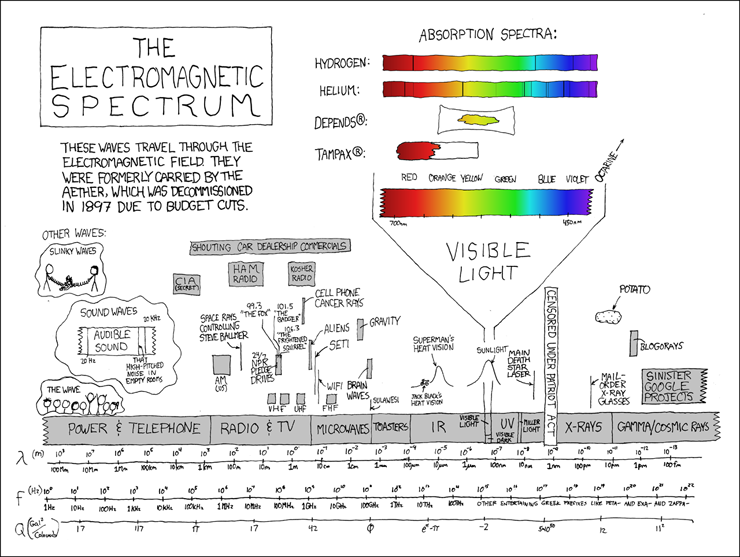
\includegraphics[width=1\linewidth]{figures/electromagnetic_spectrum_small}
		\end{center}
		\flushright -- Randall Munroe, \href{https://xkcd.com/273/}{XKCD\#273}
	}
	
	%----------------------------------------------------------------------------------------
	%	OUTPUT TITLE PAGE AND PREVIOUS
	%----------------------------------------------------------------------------------------
	
	% Note that \maketitle outputs the pages before here
	
	% If twoside=false, \uppertitleback and \lowertitleback are not printed
	% To overcome this issue, we set twoside=semi just before printing the title pages, and set it back to false just after the title pages
	\KOMAoptions{twoside=semi}
	\maketitle
	\KOMAoptions{twoside=false}
	
	%----------------------------------------------------------------------------------------
	%	RESUME
	%----------------------------------------------------------------------------------------
	
	\chapter*{Summary}
Summary and keywords
%\selectlanguage{french}

%\vspace{0.5cm}
%Mots clés: géométrie algorithmique, complexe planaire et rectangulaire, géodésique, courbure globale non-positive

%\selectlanguage{english}


	
	%----------------------------------------------------------------------------------------
	%	TABLE OF CONTENTS & LIST OF FIGURES/TABLES
	%----------------------------------------------------------------------------------------
	
	\begingroup % Local scope for the following commands
	
	% Define the style for the TOC, LOF, and LOT
	%\setstretch{1} % Uncomment to modify line spacing in the ToC
	%\hypersetup{linkcolor=blue} % Uncomment to set the colour of links in the ToC
	\setlength{\textheight}{23cm} % Manually adjust the height of the ToC pages
	
	% Turn on compatibility mode for the etoc package
	\etocstandarddisplaystyle % "toc display" as if etoc was not loaded
	\etocstandardlines % "toc lines as if etoc was not loaded
	
	\tableofcontents % Output the table of contents
	
	%\listoffigures % Output the list of figures
	
	% Comment both of the following lines to have the LOF and the LOT on different pages
	%\let\cleardoublepage\bigskip
	%\let\clearpage\bigskip
	
	%\listoftables % Output the list of tables
	
	\endgroup
	
	%----------------------------------------------------------------------------------------
	%	MAIN BODY
	%----------------------------------------------------------------------------------------
	
	\mainmatter % Denotes the start of the main document content, resets page numbering and uses arabic numbers
	
	\setchapterstyle{kao}
%\setchapterpreamble[u]{\margintoc}
\chapter{Summary}
\labch{intro}

Magnetic confinement fusion researches is the most advanced technique to master nuclear fusion for energy production. One of the main requirements for achieving fusion is to heat the plasma particles to temperatures exceeding 100-200 million of degrees (10-20 keV). Electromagnetic waves in mega-watt range of power, from tens of MHz to hundreds of GHz, are launched by antennas located near the plasma periphery in order to increase the plasma temperature and extend its duration \sidecite{Cairns1991}. 




Part of my work is not described in thus manuscript, like some analysis concerning RF plasma cleaning in the frame of the ITER Wide-Angle Visible (WAVS) diagnostic, my work as WEST Engineer-in-Charge (\href{https://github.com/IRFM/PPPAT/}{https://github.com/IRFM/PPPAT/}) and a rapid excursion in the Electron Cyclotron world (\cite{farthouat2010}). 


Some figures in this manuscript, like Figure~\ref{fig:chap1:reactivity} and Figure~\ref{fig:chap1:nTtau_machines} have been made in the frame on an \href{https://github.com/alfkoehn/fusion_plots/}{open-source project} created in collaboration with Alf Koehn from University of Stuttgart, which purpose is to reproduce classic figures used in Fusion Textbooks using open-source codes and data.
	
%	 % Page avec titre seul
%	\pagelayout{wide} % No margins
%	\addpart{intro}
%	\pagelayout{margin} % Restore margins
	
	% Fusion and tokamak
	% controlled fusion and RF heating and current drive
%\chaptertoc{}

\chapter{Controlled Fusion, RF heating and Current Drive}

%%%%%%%%%%%%%%%%%%%%%%%%%%%%%%%%%%%%%%%%%%
%%%%%%%%%%%%%%%%%%%%%%%%%%%%%%%%%%%%%%%%%%
\section{Nuclear Fusion}
Nuclear fusion is the process that powers all the stars in the Universe, including our Sun. To get nuclear fusion, nuclei have to come close enough to each other where nuclear forces can overcome their mutual electrostatic repulsion. This would require temperatures of the order of 720 keV for head-on collisions of thermal particles to lead to fusion reactions in a classical way. 
Actually, quantum physics has to be taken into account in the process. Both in tokamaks and in stars interiors, fusion reactions take place predominantly due to the tunnel effect. Crossing this barrier can be quantified in a probabilistic manner with the reaction rate $R$ $[\mathrm{reaction/m^3 s}]$, defined as the probability of reaction per unit time and volume. 
The reaction rate between mono-energetic ions of density $n_1$ $\mathrm{[m^{-3}]}$ striking target ions of density $n_2$ $\mathrm{[m^{-3}]}$ is proportional to the effective cross-section area $\sigma$ $\mathrm{[m^2]}$ and to the velocity difference $v_{12}$ between the two species:
\begin{equation*}
	r_{12} = n_1 n_2 \; \sigma v_{12}
\end{equation*}
The quantity  $\sigma v_{12}$, which depends on the kinetic energy of the colliding particles, is called the reactivity ($\mathrm{[m^3/s]}$). The reaction rate $r_{12}$ is proportional to the square of the density of the mixture. In fusion plasmas, ions are not mono-energetic. They are assumed to have Maxwellian velocity distributions. The average reactivity $\langle \sigma v \rangle_{12}$ derives from the following expression:
\begin{equation*}
	\left < \sigma v \right >_{12} 
	= \int_{-\infty}^{+\infty} \int_{-\infty}^{+\infty} 
	\sigma(v_{12}) v_{12}\;  f_1(v_1) f_2(v_2) \; dv_1dv_2
\end{equation*}

Finally, the average reaction rate $R_{12}$ reads:
\begin{equation*}
	R_{12} = n_1 n_2 \; \left < \sigma v \right >_{12}
\end{equation*}
It governs the time evolution of both densities: $\dv{n_1}{t} = \dv{n_2}{t} = - R_{12}$. The temperature dependence of the reactivity $\langle \sigma v \rangle_{12}$ is plotted on figure \ref{fig:chap1:reactivity} for several fusion reactions.

\begin{figure} 
	\begin{center}
		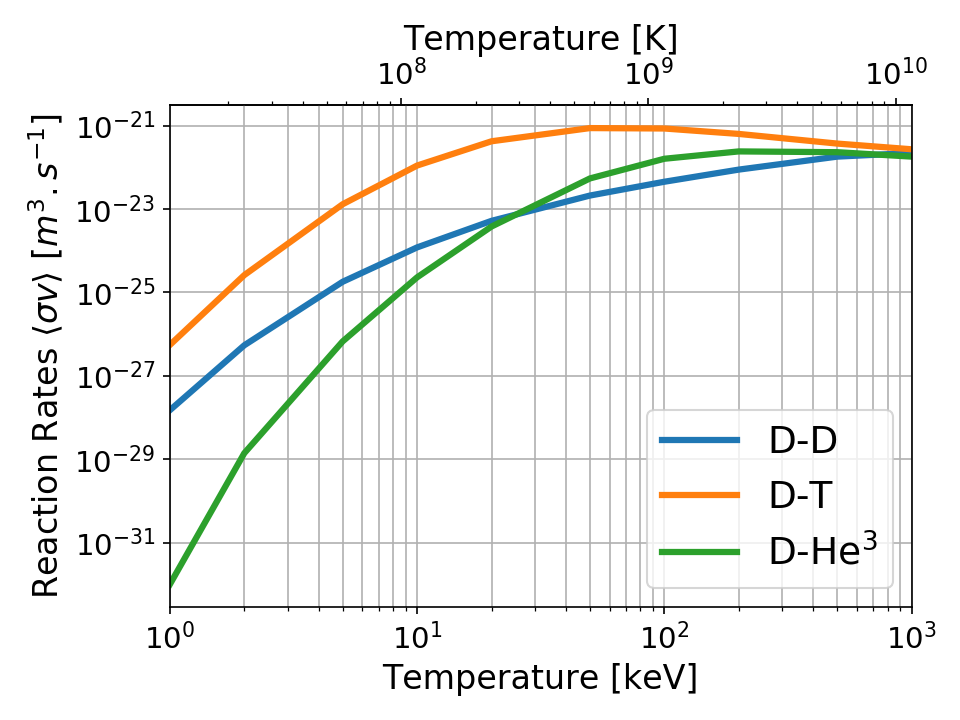
\includegraphics[width=1.0\textwidth]{figures/chap1/Fusion_Reactivity.png}
		\caption{Fusion reactivity versus temperature for few couples of fusion reactions. Data from \citeauthyear{richardson2019}.}
		\label{fig:chap1:reactivity}
	\end{center}
\end{figure}

The D-T reactivity reaches its maximum for a temperature of 64 keV, corresponding to a temperature of $742\,10^6$ K. Since it has the highest reaction rate, the D-T reaction is the “easiest” to initiate (maximum reactivity at lowest temperature) of all fusion reactions and is the main targeted reaction for controlled fusion reactors\sidecite{cea1987, ball2019}: 
\begin{equation*}
	\mathrm{D + T} \longrightarrow \mathrm{{}^4 He~(3.56~MeV) + n~(14.03~MeV)}
\end{equation*}
Therefore, the D-T reaction leads to a total released energy of $E_{DT}$ = 17.59 \si{MeV} = $2.82\times 10^{-12} \si{J}$ per fusion reaction\sidenote{This value can be compared to the 200~MeV released by $^{235}$U fission. Yet, the energy release \emph{per nucleon} ($i.e.$ per kilogram) is approximately 4 times larger for fusion than for fission reactions.}.

The fusion power per unit volume $p_{DT}$ produced by the fusion of the nuclei of deuterium and tritium reads: 
\begin{equation*}
	P_{fus} = n_D n_T \left< \sigma v \right>_{DT} E_{DT}
\end{equation*}
with $n_D$ and $n_T$ the deuterium and tritium density and $\left< \sigma v \right>_{DT}$ the D-T reactivity. 


The fusion power per unit volume $p_{DT}$ produced by the fusion of the nuclei of deuterium and tritium reads: 
\begin{equation*}
p_{DT} = n_D n_T \left< \sigma v \right>_{DT} E_{DT}
\end{equation*}
with $n_D$ and $n_T$ the deuterium and tritium density and $\left< \sigma v \right>_{DT}$ the D-T reactivity. Assuming equal deuterium and tritium densities:
\begin{equation*}
n_D = n_T = \frac{n}{2}
\end{equation*}
with $n$ the electron density, then the thermonuclear power density is:
\begin{equation*}
p_{DT} = \frac{1}{4} n^2 \left< \sigma v \right>_{DT} E_{DT}
\end{equation*}

%Assuming a constant reactivity in the plasma ("flat profile hypothesis") and using the tore volume $V$, the fusion power is: 
%\begin{equation}
%P_{fus} = \frac{V}{4}
%n^2 \left< \sigma v \right>_{DT} E_{DT}
%\end{equation}
%
%For a circular cross-section, the plasma volume is $V=2\pi^2 R a^2$. The reactivity $\left< \sigma v \right>_{DT}$ depends on the temperature. In the temperature range 10.3-18.5 keV, it turns out that the reactivity $\left< \sigma v \right>_{DT}$ can well (with about 10$\%$ error) be approximated by \sidecite{wesson2011}: 
%\begin{equation*}
%	\left< \sigma v \right>_{DT} \approx 1.18\, 10^{-24}\; \hat T^2 \;\si{\left[m^3 s^{-1}\right]}
%\end{equation*}
%where $\hat T$ is expressed in $\si{keV}$.

%%%%%%%%%%%%%%%%%%%%%%%%%%%%%%%%%%%%%%%%%%
\section{Magnetic Controlled Fusion}
If controlled in a reactor, fusion power could be an ideal energy source. It would run on hydrogen isotopes (such as deuterium which can be found in sea water and tritium which can be generated inside the reactor), does not generate greenhouse gas and creates no radioactive waste except the reactor vessel itself. It would require much less land mass than wind or solar power installations for similar power and could produce power 24/7. But producing a self-sustaining fusion reaction requires that deuterium and tritium be heated to over 150 million K, a temperature at which they become plasma: an electrically charged gas. 


Sustaining a high temperature in steady-state requires that the plasma be confined by magnetic field. The magnetic device called \emph{tokamak}, first developed in the Soviet Union in the early 1960s, is an efficient way to confine high temperature plasmas\sidecite{shafranov2001, azizov2012, mirnov2019}. It is an axially symmetric field configuration 

, generated by superconducting electromagnets. 






\subsection{Ohmic Heating}
%%%%%%%%%%%%%%%%%%%%%%%%%%%%%%%%%%%%%%%%%%

\subsection{Radio frequency Heating and Current Drive}
%%%%%%%%%%%%%%%%%%%%%%%%%%%%%%%%%%%%%%%%%%
\section{Ion Cyclotron Resonance Frequency}

%%%%%%%%%%%%%%%%%%%%%%%%%%%%%%%%%%%%%%%%%%
%%%%%%%%%%%%%%%%%%%%%%%%%%%%%%%%%%%%%%%%%%
\section{Lower Hybrid Resonance Frequency}
Originally, the occurrence of a wave resonance, the \emph{lower hybrid resonance}, has been anticipated to lead to strong wave-particle interaction through linear and non-linear mode conversion to a hot plasma wave\sidecite{stix1992}. With an appropriate RF launcher conceived to excite cold plasma waves, these would propagate into the plasma until reaching the lower hybrid resonant layer at $\omega_{LH}$. This resonance exists in tokamak plasma in the region close to the ion plasma frequency $\omega_{pi}/2\pi$, which lies in the lower end of the microwave band (1-5~GHz). At this layer, the perpendicular group velocity vanishes and the waves can convert into a hot plasma mode which is absorbed. This heating technique, known as \emph{Lower Hybrid plasma Ion Heating} (LHIH) or \emph{Lower Hybrid Resonance Heating} (LHRH), was the originally experimentally investigated method in the 70'\sidecite{bellan1974, hooke1972, golant1972, tonon1977}. Different physical mechanisms have been invoked to explain the energy absorption, such as stochastic Ion Heating in \citeauthyear{karney1978} and quasi-linear electron Landau damping in \citeauthyear{brambilla1983}.


In the 80', effective ion heating had only been obtained in a small number of experiments and research along the application of LH waves towards bulk ion heating were slowing down\sidecite{gormezano1986, porkolab1984, tonon1984}. The reason for this is that bulk ion heating near the mode conversion layer appeared to be less reproducible and more difficult to achieve than electron heating. Indeed, as the wave frequency gets closer to the lower hybrid frequency, the shorter wavelength waves may be more effectively absorbed and/or scattered near the plasma surface by non-linear effects such as parametric instabilities, low-frequency fluctuations, etc. Moreover, for LH bulk ion heating, the unconfined ions impinging on the wall induced a large amount of metallic impurities and then the increase of power radiated by the plasma.

Rather than trying to heat ions, it was theorized postulated that high phase velocity waves travelling in the direction parallel to the magnetic field could interact quasi-linearly by Landau interaction with the electrons population, and, by using an asymmetric spectrum could drive a large amount additional of toroidal plasma current \sidecite{fisch1978}. In the same fashion that for LHRH, the RF power is coupled to the plasma via launchers made of rectangular waveguides stacked periodically in the horizontal direction parallel to the toroïdal magnetic field. However, at the contrary of LHRH launchers, the LH waves are launched preferentially in one toroidal direction by mean of a phased array. The LH wave excited by such an array has an asymmetric parallel spectrum. The LH waves create an asymmetry in the electron distribution, which ultimately results in a net electric current \sidecite{fisch1987}. This technique is known as \emph{Lower Hybrid Current Drive} and despite the fact that the Lower Hybrid resonance is not any more involved in the use of this method in tokamaks, the term remained. LHCD has been confirmed on the PLT tokamak in 1982 \sidecite{bernabei1982} and in Alcator-C in 1984 \sidecite{porkolab1984}. 

Since in 1982 many impressive results were presented on LHCD\sidecite{stevens1982, stevens1983, porkolab1984, tonon1983} toward steady state or quasi steady state tokamak operations, most LH experiments were dedicated to electron interaction and especially to current drive. A recent review of LHCD is available in \sidecite{bonoli2014}.

Currently, the LH waves term refers to the waves which satisfy the slow-wave branch of the cold plasma dispersion relation for parallel index larger than one ($|n_{\parallel}|>1$) and a RF frequency $\omega$ which lies between the ion cyclotron $\omega_{ci}$ and the electron cyclotron $\omega_{ce}$ frequencies. 

%For the LH method which operates at the lower end of the microwave band (1-5 GHz) klystrons transform electrical power into electromagnetic power (step 1), which is transported to the plasma using waveguides (step 2). The power is coupled to the plasma with antennas called "grills" because of their characteristic shape (step 3), transported inside the plasma by plasma waves (typically the slow wave) (step 4), and absorbed on ions or electrons by wave-particle interaction (step 5).


	
	% RF fundamentals
	% #####################################################
% #####################################################
% #####################################################
\setchapterpreamble[u]{\margintoc}
\chapter{RF Fundamentals}\label{chap:RF_fundamentals}


\epigraph{It is not knowledge, but the act of learning, not possession but the act of getting there, which grants the greatest enjoyment.}{Carl Friedrich Gauss}

This chapter is a reminder of the essential analytic elements of RF engineering used in this manuscript. Readers already aware of the transmission line and electromagnetic network theory can skip this chapter.

We will review the fundamentals of transmission line theory (Section~\ref{sec:transmission_line}), generalities about matching systems (Section~\ref{sec:matching_systems}) and scattering parameters (Section~\ref{sec:s-parameters}). Then, we will detail some particular results concerning coaxial lines (Section~\ref{sec:coaxial_lines}) and rectangular waveguides (Section~\ref{sec:rectangular_waveguide}). 

% #####################################################
% #####################################################
% #####################################################
\section{Uniform Transmission lines Properties}\label{sec:transmission_line}
\marginnote[*-2]{Part of this section are taken from the documentation of the open-source Python package \href{http://scikit-rf.org/}{scikit-rf} which is maintained by the author and used in RF circuit models, for example in \citeauthyear{hillairet2015-2} or in \citeauthyear{hillairet2019-1}.}

Once RF waves have been generated, it must be transmitted to the antennas, using suitable transmission line depending on the RF frequency and power level. The main results and properties of uniform transmission lines are reviewed in this section. The results given here are well-known and can be found in numerous textbooks such as \sidecite{Harrington2001, marcuvitz1951, Thourel1988, Collin1990, gonzalez1997, pozar2012, Orfanidis, steer2019-3} to give a personal selection.

A transmission line is defined as \textit{uniform} if its dimensions and electrical properties are identical for all planes transverse to the direction of propagation. The results listed in this section are used in the following sections of this chapter for the design and the analysis of high power RF components.

% #####################################################
\subsection{Voltage and Current}

\begin{figure}
	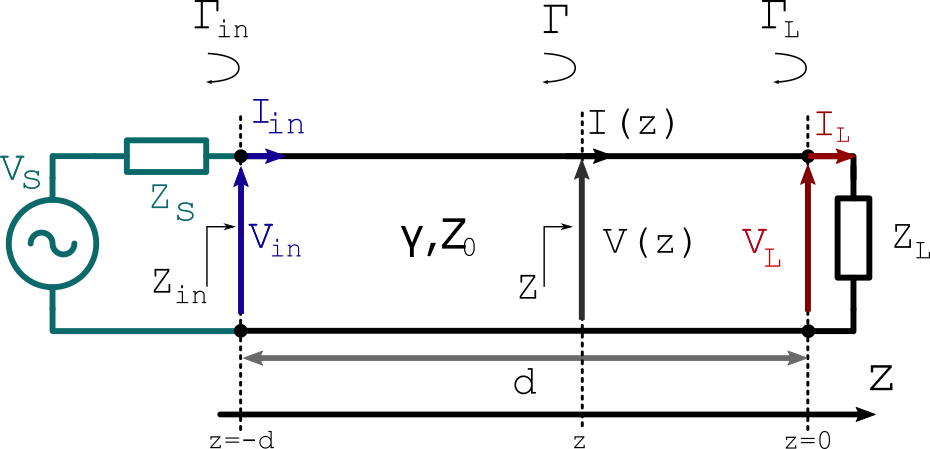
\includegraphics[width=1.0\textwidth]{figures/chap3/transmission_line_properties_vi}
	\caption{A transmission line terminated in a load impedance $Z_L$.}
	\label{fig:transmissionlinepropertiesvi}
\end{figure}

Let a lossy transmission line of propagation constant $\gamma=\alpha+j\beta$ (in $\si{m^{-1}}$) and characteristic impedance $Z_0$ (in $\si{\Omega}$), terminated by an arbitrary load $Z_L$. The line length is The source is parametrized by the distance $z$, where the source is located at distance $z=-d$ from the load ($z=0$) as illustrated in Figure~\ref{fig:transmissionlinepropertiesvi}. Attenuation constant $\alpha$ has the units of Nepers per meter $\si{Np/m}$ and the phase constant $\beta$ has the units radians per meter $\si{rad/m}$\footnote{$1\,\si{Np/m}$ equals to $8.6859 \, \si{dB/m}$. To convert from \si{dB} to \si{Np} multiply by $0.1151$. Thus $\alpha = x \, \si{dB/m} = x \times 0.1151 \, \si{Np/m}$.}. Let $V=V(z)$ and $I=I(z)$ the total voltage and current on the line, which can be written as a sum of a forward and reflected waves:
\marginnote{$\Vfwd$ and $\Vrefl$ ($\Ifwd$ and $\Irefl$) are defined here as peak voltages (currents). For sine wave, RMS voltage is $V_{\mathrm{RMS}}=V_{\mathrm{peak}}/\sqrt{2}$.}
\begin{subequations}
\begin{align}
	V(z) = \Vfwd(z) + \Vrefl(z) =& \Vfwd e^{-\gamma z} + \Vrefl e^{+\gamma z} \\
	I(z) = \Ifwd(z) + \Irefl(z) =& \frac{\Vfwd}{Z_0} e^{-\gamma z} - \frac{\Vrefl}{Z_0} e^{+\gamma z}
\end{align}
	\label{eq:voltage_current_lossy_line}
\end{subequations}
where the $e^{-\gamma z}$ term represents wave propagation in the $+z$ direction (and $e^{+\gamma z}$ in the $-z$ direction). The terms $\Vfwd$, $\Vrefl$ ($\Ifwd$, $\Irefl$) represent the forward and reflected voltage (current) waves at $z=0$.  
The \textit{characteristic impedance} $Z_0$ associated to a uniform transmission line (or any continuous media supporting the propagation of electromagnetic waves) is defined as the ratio of the forward voltage and current when the transmission line is infinite, i.e.  $Z_0=\Vfwd/\Ifwd(=-\Vrefl/\Irefl)$. It characterizes the property of the line to oppose a change in voltage for a change of current or vice-versa. When $Z_L=Z_0$, the load is said to be \textit{matched} to the line and there is no reflected wave $\Vrefl=0$.

\begin{marginfigure}[-2cm]
	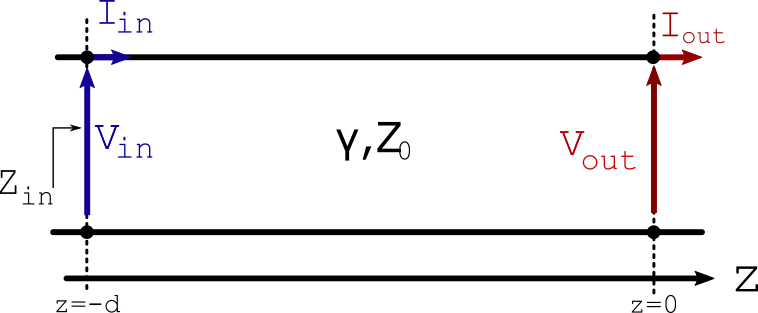
\includegraphics[width=1\linewidth]{figures/chap3/transmission_line_transfer}
	\caption{Propagation of current and voltage in a piece of uniform transmission line.}
	\label{fig:transmission_line_transfer}
\end{marginfigure}

The voltage and current at the input ($z=-d$) of a piece of uniform transmission line can be related to the voltage and current at its output (chosen at $z=0$) using the transfer matrix \sidecite{vittoria1998}:
\begin{equation}
\left( 
\begin{array}{c}
	V_{\mathrm{in}} \\
	I_{\mathrm{in}}
\end{array}
\right)
=
\left( 
\begin{array}{cc}
\cosh  \left(\gamma d\right) & Z_0 \sinh \left(\gamma d \right) \\ 
\frac{1}{Z_0}\sinh \left( \gamma d\right) & \cosh\left(\gamma d\right) 
\end{array} 
\right)
\left( 
\begin{array}{c}
	V_{\mathrm{out}} \\
	I_{\mathrm{out}}
\end{array}
\right)
	\label{eq:voltage_current_transfer_matrix}
\end{equation}




% #####################################################
\subsection{Reflection Coefficient}
The ratio of the reflected to forward voltage (or current) at a distance $z$ defines the \textit{reflection coefficient} $\Gamma$:
\marginnote{\textit{Return loss} RL is the negative of the magnitude of the reflection coefficient in \si{dB}. Since power is proportional to the square of the voltage, return loss is given by $$\mathrm{RL} = -20 \log_{10} |\Gamma|$$
The \textit{transmission coefficient} can be also defined as $$T=1+\Gamma$$
 sometime expressed as the \textit{insertion loss} IL in \si{dB}:
 $$\mathrm{IL}=-20 \log |T|$$}
\begin{equation}
\Gamma(z) = \frac{\Vrefl(z)}{\Vfwd(z)} =  \frac{\Irefl(z)}{\Ifwd(z)} = \Gamma_L e^{2\gamma z}
\label{eq:Gamma_at_z}
\end{equation}
where $\Gamma_L$ is the reflection coefficient of the load ($z=0$), given by:
\begin{equation}
	\Gamma_L = \frac{Z_L - Z_0}{Z_L + Z_0}
	\label{eq:Gamma_L}
\end{equation}
Note that the reflection coefficient at the input of the line $\Gamma_{\mathrm{in}}$ (Figure~\ref{fig:coaxial_line_fields}) is given for $z=-d$:
$$
\Gamma_{\mathrm{in}}=\Gamma(z=-d)=\Gamma_L e^{-2\gamma d}
$$

In fusion application, the load is unfortunately rarely matched to the transmission line or the source impedances, so it is convenient to re-express voltage and current equations (\ref{eq:voltage_current_lossy_line}) as a function of $\Gamma_L$ (\ref{eq:Gamma_L}) or $\Gamma(z)$ (\ref{eq:Gamma_at_z}):
\begin{subequations}
	\begin{align}
		V(z) =& \Vfwd \left( e^{-\gamma z} + \Gamma_L e^{+\gamma z} \right) 
			= \Vfwd \left[ 1 + \Gamma(z) \right]  e^{-\gamma z} \\
		I(z) =& \frac{\Vfwd}{Z_0} \left( e^{-\gamma z} - \Gamma_L e^{+\gamma z} \right)
			= \frac{\Vfwd}{Z_0} \left[ 1 - \Gamma_L(z)  \right]e^{-\gamma z}
	\end{align}
	\label{eq:voltage_current_lossy_line_gamma}
\end{subequations} 

The \textit{standing wave ratio} or SWR is defined as:
\marginnote[*-1]{With the inverse expression
	$$ 	|\Gamma| = \frac{\SWR - 1}{\SWR + 1} $$}
\begin{equation}
	\SWR(z) = \frac{1 + |\Gamma(z)|}{1 - |\Gamma(z)|}
	\label{eq:SWR}
\end{equation}
The SWR can be equivalently defined as the ratio of maximum (forward and backward waves are in phase) to minimum (forward and reflected waves are out of phase) voltage magnitudes: 
\begin{equation}
\SWR(z) = \frac{|V_\mathrm{max}(z)|}{|V_\mathrm{min}(z)|} = \frac{|\Vfwd|e^{-\alpha z} + |\Vrefl|e^{+\alpha z}}{|\Vfwd|e^{-\alpha z} - |\Vrefl|e^{+\alpha z}}
\label{eq:SWR_max_to_min_voltages}
\end{equation}
Note that the SWR becomes constant for lossless lines. 


Finally, some special cases are reminded for convenience in the Table~\ref{tab:special_case_loaded_line}.

\begin{table}[h]
	\begin{center}
\begin{tabular}{|c|c|c|}
	\hline 
	Case & $\Gamma$ & $\SWR$ \\ 
	\hline 
	Matched: $Z_L = Z_0$ & 0 & 1 \\ 
	\hline 
	Short: $Z_L=0$ & -1 & $\infty$ \\ 
	\hline 
	Open: $Z_L = \infty$ & 1 & $\infty$ \\
	\hline
\end{tabular}
	\end{center}
\caption{Special cases of a uniform loaded transmission line.}
\label{tab:special_case_loaded_line} 
\end{table}


% #####################################################
\subsection{Line Impedance}
The impedance seen toward the load at a point of the line, that is the ratio between total voltage and current at this point, is at a distance $z=-\ell$ from the load:
\begin{subequations}
	\begin{align}
Z(z=-\ell) 
	=& Z_0 \frac{Z_L + Z_0 \tanh( \gamma \ell)}{Z_0 + Z_L \tanh(\gamma \ell)} \\
	=& Z_0 \frac{1 + \Gamma(-\ell) }{1 - \Gamma(-\ell) }
	\end{align}
\end{subequations}
As noted aboved with respect to Figure~\ref{fig:coaxial_line_fields}, we have in particular $Z_{\mathrm{in}}=Z(z=-d)$ and $Z(z=0)=Z_L$.

% #####################################################
\subsection{Power and losses}\label{sec:power_and_losses}
The time average power flowing along the transmission line is the difference between the forward and the reflected powers:
\begin{equation}
P (z) = \frac{1}{2} \Re\left[V(z) I^*(z)\right] 
\label{eq:power_time_average_general}
\end{equation}

\marginnote{An example in the \href{https://scikit-rf.readthedocs.io}{scikit-rf package documentation} is dedicated to the evolution of the power, voltage, current and SWR in lossy line. See \cite[§2.7]{pozar2012}, \cite[§2.5.5]{steer2019}, \cite[§3-4c]{Rizzi1988} for discussions of power in lossy terminated line.}

For a lossy transmission line ($\alpha>0$), not all the power entering the transmission line will be delivered to the load as some power will be lost on the line due to attenuation. The time average power at any point of the transmission line (\ref{eq:power_time_average_general}) can be shown to be \sidecite[+1cm]{vernon1969, marks1992}:
\begin{subequations}
\begin{align} 
	P(z) =& P_\mathrm{f} - P_\mathrm{r} - P_\mathrm{c} \\
	P_\mathrm{f} =& \Re(Z_0) \frac{|V_\mathrm{f}|^2}{2 |Z_0|^2} e^{-2\alpha z} \\
	P_\mathrm{r} =& \Re(Z_0) \frac{|V_\mathrm{r}|^2}{2 |Z_0|^2} e^{+2\alpha z} = P_\mathrm{f} |\Gamma_L|^2 e^{+4\alpha z} \\
	P_\mathrm{c} =& \Im(Z_0) \Im\left[\frac{\Vrefl\Vfwd^*}{|Z_0|^2} e^{-2j\beta z} \right]
\end{align}
\end{subequations}
where $P_\mathrm{f}$ and $P_\mathrm{r}$ are the forward and reflected power respectively. In lossy lines, the net power flow $P(z)$ is not in general the difference of the forward and reflected power but carries an additional term $P_\mathrm{c}$. $P_\mathrm{c}$ can be either positive or negative along the line and is null for all $z$ only for a distortion-less line ($\Im(Z_0)=0$). In a word, the superposition of power does not apply in lossy uniform transmission lines (but superposition of voltages and currents does).

Keeping the notation used in Figure~\ref{fig:transmissionlinepropertiesvi} and using equations (\ref{eq:voltage_current_lossy_line_gamma}), the power delivered to the load (at position $z=0$) and at the input of the line (at position $z=-d$) are:
\begin{subequations}
	\begin{align}
		P_{\mathrm{L}} = P(z=0) =& \Re(Z_0) \frac{\left| \Vfwd \right|^2}{2 |Z_0|^2} \left(1 - |\Gamma_L|^2 \right) \\
		P_{\mathrm{in}} = P(z=-d) =& \Re(Z_0) \frac{\left| \Vfwd \right|^2}{2 |Z_0|^2} \left(1 - |\Gamma_L|^2 e^{-4\alpha d}  \right) e^{2\alpha d}
	\end{align}
\end{subequations}
hence the power lost in the line is:
\marginnote{The total loss $\mathrm{ML}$ in a line in \si{dB} can also be stated as:
$$
 \mathrm{TL}=10\log_{10} \left( \frac{A^2 - |\Gamma_L|^2}{A(1 - |\Gamma_L|^2)} \right)
$$
where $A=10^{\mathrm{ML}/10}$ and $\mathrm{ML}$ the matched line loss. The additional loss caused by the standing waves is the difference between the  $\mathrm{TL}$ and  $\mathrm{ML}$.
}
\begin{equation}
P_{\mathrm{loss}} = P_{\mathrm{in}} - P_{\mathrm{L}} 
= \Re(Z_0)  \frac{\left| \Vfwd \right|^2}{2 |Z_0|^2} 
\left[ 
\left(e^{2\alpha d} - 1\right) + |\Gamma_L|^2 \left( 1 - e^{-2\alpha d} \right)
\right]
\label{eq:power_loss_lossy_transmission_line}
\end{equation}
where the first and second terms in (\ref{eq:power_loss_lossy_transmission_line}) account for the power loss of the forward and reflected waves respectively.
	


For lossless transmission line and real characteristic impedance, the time average power flow along the transmission line is constant and (\ref{eq:power_time_average_general}) simplifies to:
\begin{equation}
P = P_\mathrm{f} - P_\mathrm{r} = P_\mathrm{f} \left(1 - |\Gamma_L|^2\right)
\label{eq:power_loss_lossless_transmission_line}
\end{equation}
This power can also be related to the maximum voltages or currents and $\SWR$ from Eq.(\ref{eq:SWR_max_to_min_voltages}):
\begin{equation}
P = P_\mathrm{f} - P_\mathrm{r} = \frac{1}{2 Z_0} \frac{	|V_{\mathrm{max}}|^2}{\SWR} = \frac{Z_0}{2} \frac{|I_{\mathrm{max}}|^2}{\SWR}
\label{eq:power_loss_lossless_transmission_line_maxvoltage_maxcurrent}
\end{equation}
where $|V_{\mathrm{max}}| = \max_z |V(z)| = |\Vfwd| + |\Vrefl|$ and similarly for $|I_\mathrm{max}|$. Combining the above two expressions leads to convenient formulas for heat flux and breakdown estimations, which relates the maximum (peak) voltage or current to the forward power $P_\mathrm{f}$ and reflection coefficient $|\Gamma_L|$:
\begin{subequations}
	\begin{align}
		|V_\mathrm{max}| =& \sqrt{2 Z_0 P_\mathrm{f} } \left(1 + |\Gamma_L| \right) \\
		|I_\mathrm{max}| =& \sqrt{\frac{2 P_\mathrm{f}}{Z_0} } \left(1 + |\Gamma_L| \right)
	\end{align}
	\label{eq:max_current_function_forward_power_gammaL}
\end{subequations}

The power lost in the transmission line is converted into heat in the metallic conductors and dielectric elements due to Ohmic and dielectric losses respectively. For high power applications such as RF heating and current drive, this heat must be evacuated to sustain CW operation. Before expressing loss formulas for the main two kinds of transmission lines used for ICRH and LHCD, we recall here for future references that the power loss in a good conductor can be calculated as:
\begin{equation}
P_\ell = \frac{R_s}{2} \int_S |J_s|^2 \diff S = \frac{R_s}{2} \int_S |H_t|^2 \diff S 
\label{eq:power_loss_conductor}
\end{equation}
where the integral is performed over the conductor surface(s), $J_s$ and $H_t$ the surface current and the tengential magnetic field respectively\cite[§1.7]{pozar2012}. 

definition of the \textit{skin depth} $\delta_s$ (in $[\si{m}]$) as:
\begin{equation}
\delta_s 
	=
	\sqrt{\frac{2}{\omega \mu \sigma}}
	\label{eq:skin_depth}
\end{equation}
and the \textit{sheet resistance} $R_s$ (in $[\si{\Omega}]$) as:
\begin{equation}
R_s 
	= 
	\frac{1}{\delta_s \sigma}
	=
	\sqrt{\frac{\omega\mu}{2\sigma}}
	=
	\sqrt{\pi f \rho \mu }
	\label{eq:sheet_resistance}
\end{equation}
with $\sigma=1/\rho$ the metal conductivity (in $[\si{S/m}]$) and $\sigma$ the metal resistivity (in $[\si{\Omega m}]$). 

% #####################################################
% #####################################################
\section{Matching Systems}\label{sec:matching_systems}
In high power RF systems for fusion applications, the load is ultimately the plasma facing the antennas. As seen in Section~\ref{sec:icrh} and Section~\ref{sec:lhcd}, the plasma loading impedance is generally small compared to antenna and transmission line. Hence, a significant amount of RF power will be reflected toward the generators. It is essential to protect high power RF sources (tetrodes, klystrons) from reflected power (output mismatch). Reflected power perturbs the source impedance, the output amplitude and phase and creates higher dissipation losses\sidecite[-1cm]{pompon2012}. It can also lead to the failure of RF windows \sidecite[-+0.5cm]{ikeda1989} or even damage the tube itself\sidecite{gold1997,carter2005,benford2007}. 

Unfortunately, the plasma characteristics depend on the machine setup but also on its history, hence its RF load properties are relatively little known in advance. In addition, plasma intrinsic instabilities, such as Edge Localized Modes (ELMs), can also induce strong and fast load variations in front of the antenna, which may affect strongly the generator performances for the aforementioned reasons\sidecite{braun1995, beaumont1996} or generate breakdown in antennas and transmission lines due to peak voltage increases \sidecite{bobkov2003-1, goniche2012-2}. 

\begin{marginfigure}[*+5]
	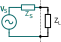
\includegraphics[width=0.8\linewidth]{figures/chap3/transmission_line_matching}
	\caption{Matching a load impedance $Z_L$ to a source having an internal impedance $Z_S$.}
	\label{fig:transmission_matching}
\end{marginfigure}

Let us consider the simplified network illustrated in Fig.\ref{fig:transmission_matching}. Classical results of RF engineering state that\cite{Rizzi1988, pozar2012}:
\begin{itemize}
	\item Conjugate Matching: maximum available power goes into the load if $Z_L=Z_S^*$
	\item Impedance Matching: minimum reflection ($\Gamma_L=0, \SWR=1$) is obtained for $Z_L=Z_S$
\end{itemize} 
As in typical plasma application the load impedance $Z_L$ is complex-valued, achieving both objectives at the same time is not possible. For this reason, a set of matching networks must be inserted between the source and the load as illustrated in Fig.~\ref{fig:transmission_matching_system}. Ideally, such a matching system should meet the following objectives (sometimes interrelated):
\begin{itemize}
	\item maximize the power transfer to the antenna 
	\item minimize the power reflected to the generator (protection and efficiency)
	\item minimize the power lost in the transmission line (net efficiency)
	\item insure the good control of the antenna amplitude/phase
\end{itemize}

If the generator is not equipped with internal matching network, it is a good engineering practice to place a matching network as close as possible from its output. Similarly, placing a matching network as close as possible from the load reduce the standing waves and thus the peak current (dissipation problems) and the peak voltage (corona and breakdown problems) in the transmission line between the source and the load \cite[§4]{Rizzi1988}.

\begin{figure}
	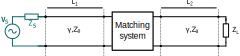
\includegraphics[width=1\linewidth]{figures/chap3/transmission_line_matching_system}
	\caption{A matching system is inserted between the source and the load impedance.}
	\label{fig:transmission_matching_system}
\end{figure}

Matching is frequency dependant since it deals with the adjustment of reactances. The perfect impedance match can occur only at one frequency but high power sources are usually very narrowband. If the source frequency can be tuned, which is the case of ICRH generators, matching networks are designed to be tunable. Such system use stub (shunt coaxial section that ends in a movable short) and line stretchers (transmission line section that can vary its electrical distance). In theory, a one-quarter-wavelength stub in conjunction with a half-wavelength stretcher can match any impedance to the generator\sidecite{england1989}. However, the actuators of these systems rely on motors (capacitors) or hydraulic systems (tuning stub, line stretchers), so their response time is of the order to 100 milliseconds or higher, which is much slower than most uncontrolled plasma variations. For this reason, fusion RF antenna are designed to be intrinsically relatively load-tolerant, using specific feeding line or antenna design. 


% #####################################################
% #####################################################
\section{Scattering Parameters}\label{sec:s-parameters}
Voltage  $V(z)$ and current $I(z)$ as defined in Eq.(\ref{eq:voltage_current_lossy_line}) in the previous section are the "real" waves in the sense that they are linked directly to Maxwell’s equations and can be measured. For example, reflection coefficients $\Gamma(z)$ can be measured from the peaks and valleys of the electric fields of the standing wave created by the beating of forward and reflected voltages and currents in a slotted-line experiment \sidecite{marks1992, williams2013}. 

A RF \textit{network} such as the one illustrated in Fig.~\ref{fig:microwave_network}, is a system for which a closed surface separating the network from the rest of the world can be found such that it has zero current on this surface ($\hat{\mathbf{n}} \times \Ebf=0$) except over one or more input/output \textit{port} cross-section \cite[§8.3]{Harrington2001}. The electrical behaviour of linear electrical networks is often handled using impedances or admittances parameters, relating voltages to currents at each port (or reference planes). Direct measurements of these impedances or admittances of a RF network requires that the ports be terminated in either short or open circuits. However, as lead inductance and capacitance make short and open circuits difficult to obtain at RF frequencies, such terminations are often hard to realize correctly. Since power transfer is often a crucial characteristic of RF network designs, \textit{scattering parameters} (or S-parameters) are often preferred by microwave engineers since they relate the power flow of forward and reflected voltage waves at each port. Finally, scattering parameters are also well suited for describing transistors and other active devices, since short and open  terminations could result in undesired behavior, including oscillation or destruction\sidecite{steer2019-1}.

\begin{marginfigure}[*-15]
	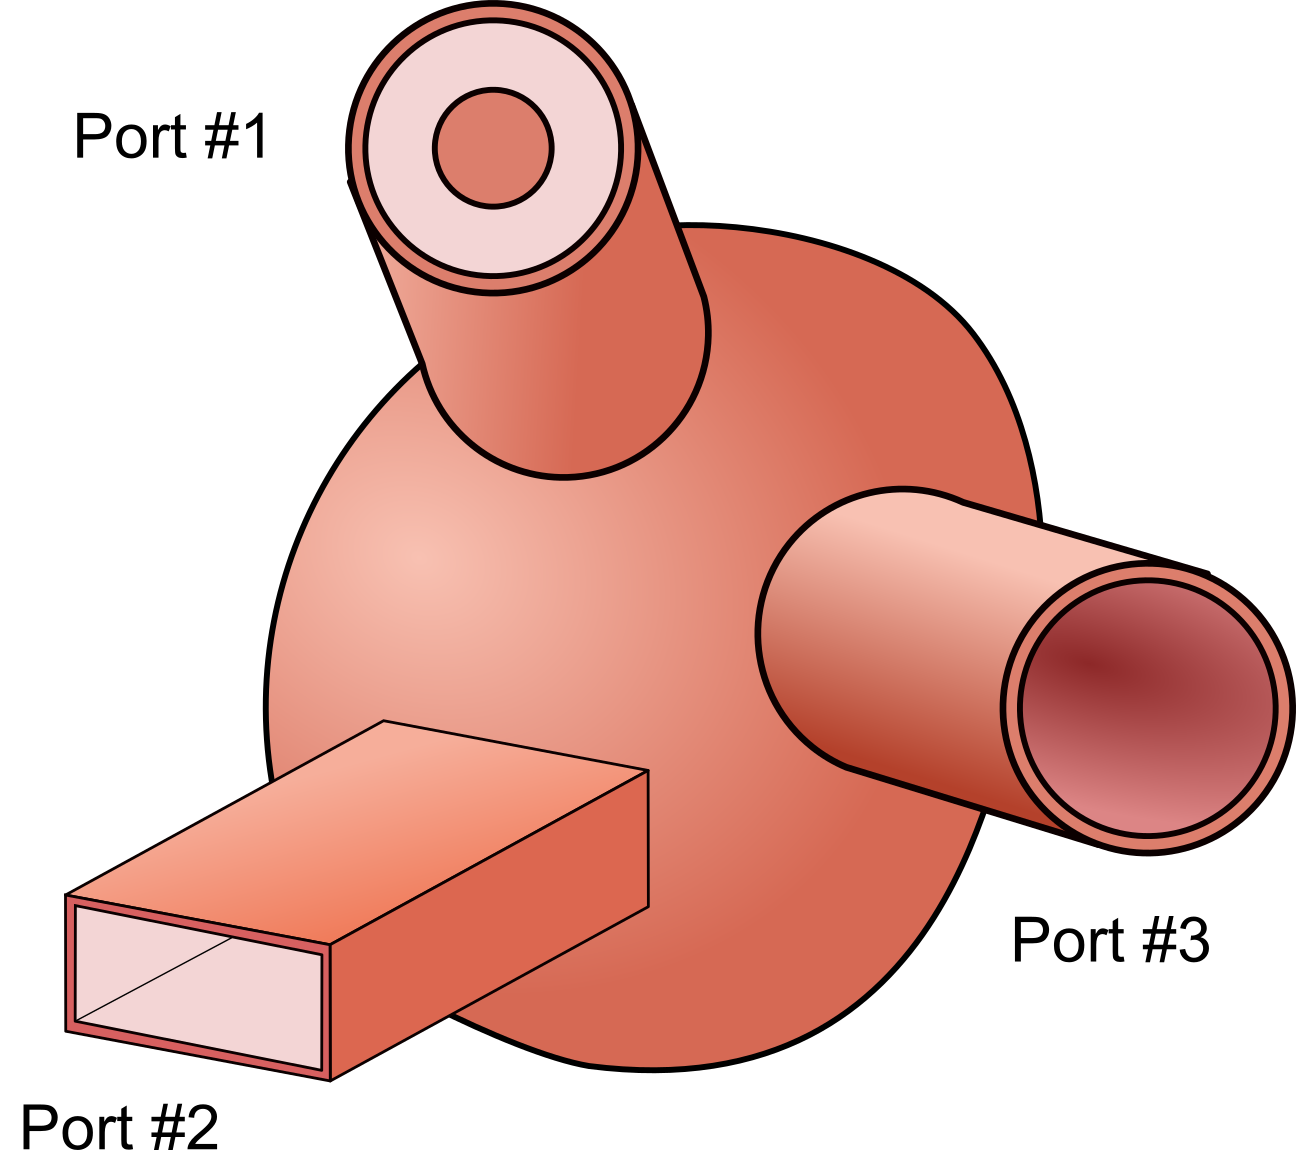
\includegraphics[width=1\linewidth]{figures/chap3/microwave_network}
	\caption{A 3 ports RF Network.}
	\label{fig:microwave_network}
\end{marginfigure}

Scattering parameters can be defined in several ways \sidecite{dobrowolski2010}, which has been discussed extensively in the literature since the 60's \cite{carlin1956, kurokawa1965, woods1972, marks1992, williams2013, amakawa2016}. Indeed, there is some arbitrariness to define some forward and reflected waves ($a, b$) such that ($|a|^2, |b|^2$) represent the time-averaged power carried by the forward and reflected voltage waves ($\Vfwd, \Vrefl$) (or current waves, or both). However, as seen in section \ref{sec:power_and_losses}, the power superposition principle does not hold for lossy lines and complex characteristic impedances (but superposition of voltages and currents does), so this mapping cannot be done in general. The various definitions of scattering parameters differ on how they handle complex impedances and eventually additional modes other than TEM, but all of these definitions give the same results for real-valued characteristic impedances and lossless lines\footnote{Because most of time lossless lines are assumed, this is probably the reason why most textbooks assume that the characteristic impedance is real in their presentation of scattering parameters. While complex-referenced S-parameters may be seen as a matter of purely academic concern with little practical use, it is not and it has also implications in electromagnetic simulators that are often silent on how they implement such situations.}. To deal with lossy lines and complex characteristic impedances, few methodologies exist but two are nowadays mostly adopted: \textit{power-wave} and \textit{pseudo-wave}  definitions. 

The \textit{power-waves} concept has been introduced in \sidecite{kurokawa1965}, where the forward $a$ and reflected $b$ power-waves are defined as:
\begin{subequations}
\begin{align}
	a =& \frac{V_i + Z_{R,i} I_i}{2\sqrt{|\Re(Z_{R,i})|}} \\
	b =& \frac{V_i - Z_{R,i}^* I_i}{2\sqrt{|\Re(Z_{R,i})|}}
\end{align}
\label{eq:power-waves_definition}
\end{subequations}
where $V_i$ and $I_i$ are the total voltage and current flowing into the $i$th port of the network. $Z_{i}$ is the $i$th port reference impedance. The choice of the reference impedance is free; a common practice is to set its value to the impedance of a load or a generator, enabling power waves to be used in matching problems. With power-waves, the power flowing at the port interface is:
\begin{equation}
	p_{\mathrm{pw}} = \frac{1}{2} \left( |a|^2 - |b|^2 \right)
\end{equation}

As seen in the previous section, impedance match and maximum power transfer are in general not coincident. For the latter condition, a conjugate match is required, i.e. when $Z_0 = Z_L^*$ using the notation of Fig.~\ref{fig:transmissionlinepropertiesvi}. Power-waves are defined in such a way that a conjugate match produces no reflection, and also in such a way that the incident wave carries the available power of the source and the reflected wave the total reflected power from the load\sidecite{woods1972}. Thus, the power-wave reflection coefficient is defined by:
\marginnote{To be compared with Eq.(\ref{eq:Gamma_L}).}
\begin{equation}
	\Gamma_{\mathrm{pw}} = \frac{Z_0 - Z_L^*}{Z_0 + Z_L}
\end{equation}

This definition introduces "wave" variables that can no longer be interpreted as incoming and outgoing waves from ports. However, they can be interpreted in terms of power flow at a junction, which explains its wide adoption by the RF community. Most RF circuit solvers (such as Keysight ADS, ANSYS Circuit) use the \textit{power-waves} definition introduced. \marginnote[*-4]{Because of its wide adoption, \href{http://scikit-rf.org/}{scikit-rf} also uses the power-waves definition by default (mostly in order to replicate results from commercial solvers) but allows the use of pseudo-wave definition as well.} 

However, the power-wave definition has some caveats one must be aware of. In particular, power-waves definition may not give physical results in case of complex characteristic impedance\footnote{A simple illustration of the problem is to consider a transmission line of complex characteristic impedance $Z_0$ loaded with a an impedance $Z_L=Z_0^*$. Voltage and current waves as defined at the beginning of this section will lead to a non zero reflection coefficient $\Gamma_L$ while power-waves-based tools will give a zero reflection coefficient $\Gamma_\mathrm{pw,L}$\cite{amakawa2016}.} and are not always continuous at the interface between circuits unless reference impedance is real, so cannot be cascaded in all cases{marks1992, williams2013}. In the real world, all transmission lines are lossy (at least to a small degree) and this contradiction has been identified shortly after Kurokawa seminal paper\cite{amakawa2016} but somewhat forgotten after. For this reason, \citeauthyear{marks1992} introduced the \textit{pseudo-waves} definition of S-parameters\footnote{where a phase factor used in \cite{marks1992} has been omitted here for simplification.}:\marginnote{Again, the pseudo-wave definition equals the travelling-wave definition when $\Zref$ is real-valued. This paragraph aims only to highlight the fact that great care should be taken when dealing with S-parameters with lossy transmission lines with electromagnetic solvers, in particular closed-source ones.}
\begin{subequations}
	\begin{align}
		a_i =& \frac{\sqrt{\Re(Z_{R,i})}}{|Z_{R,i}|} \Vfwd_i 
		= \frac{\sqrt{\Re(Z_{R,i})}}{|Z_{R,i}|} \frac{V_i + Z_{R,i} I_i}{2} \\
		b_i =& \frac{\sqrt{\Re(Z_{R,i})}}{|Z_{R,i}|} \Vrefl_i 
= \frac{\sqrt{\Re(Z_{R,i})}}{|Z_{R,i}|} \frac{V_i - Z_{R,i} I_i}{2}		
	\end{align}
\end{subequations}
where $Z_{R,i}$ is an arbitrary value which can be different from the characteristic impedance $Z_0$ of the physical transmission line at the $i$th port. $a$ and $b$ are not longer directly related to voltage and curent travelling wave and only when $Z_{R}$ equals to $Z_0$ do $a$ and $b$ correspond to actual travelling wave amplitude (normalized to unit of $\sqrt{\si{W}}$). The power $p$ transmitted by a pseudo-wave at the port interface is:
\begin{equation}
p = \frac{1}{2} \left(|a|^2 - |b|^2 - 2\Im(a^* b) \frac{\Im(\Zref)}{\Re(\Zref)} \right)
\end{equation}

For a N-port network, with both definitions, the forward and reflected waves are related by:
\begin{equation}
	\bbf = \Sbb \abf
\end{equation}
where the $\abf$ and $\bbf$ array are constituted of the $a_i$ and $b_i$ elements. Properties of S-matrices are discussed in \sidecite{gonzalez1997, dobrowolski2010} to name of few and are not covered here.




% #####################################################
% #####################################################
\section{Coaxial Lines}\label{sec:coaxial_lines}
% #####################################################
\subsection{Coaxial Lines Main Properties}
A coaxial line is made of two cylindrical conductors, the internal of radius $a$ and the external of radius $b$, encapsulated one inside the other as illustrated in Figure~\ref{fig:coaxial_line_geometry}. The space between both conductors is filled with a dielectric. In high power application, conductors are made of rigid metallic cylinder (aluminium or stainless steel) eventually copper or silver coated to reduce RF losses. The dielectric is simply (dry) air, pressurized nitrogen or vacuum to reduce dielectric breakdown. 

% #####################################################
\subsection{Electric and Magnetic Fields}
The fundamental mode in a coxial line is a TEM mode as both electric and magnetic field are transverse to the propagation direction. This mode has no cut-off and therefore coaxial can be used down to DC.

\begin{marginfigure}[*-10]
	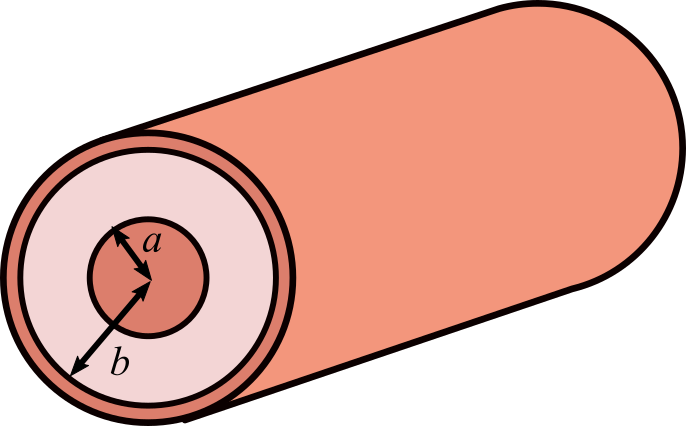
\includegraphics[width=1\linewidth]{figures/chap3/coaxial}
	\caption{Coaxial Line Geometry}
	\label{fig:coaxial_line_geometry}
\end{marginfigure}

The electric and magnetic field inside the coaxial are illustrated in Figure~\ref{fig:coaxial_line_fields} and given by:
\begin{subequations}
	\begin{align}
		\Ebf(r) =& \frac{V}{r \ln \left(b/a \right)} \hat\ebf_r \label{eq:coaxial_electric_field}\\
		\Hbf(r) =& \frac{I}{2\pi r} \hat\ebf_\phi \label{eq:coaxial_magnetic_field}
	\end{align}
	
\end{subequations}
where $V=V_0 e^{\mp\gamma z}$ is the voltage between the conductors and $I=I_0 e^{\mp\gamma z}$ is the current in each conductor, for $a\leqslant r \leqslant b$. 

\begin{marginfigure}[*-8]
	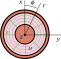
\includegraphics[width=.8\linewidth]{figures/chap3/coaxial_fields}
	\caption{TEM mode for a coaxial line}
	\label{fig:coaxial_line_fields}
\end{marginfigure}	

% #####################################################
\subsection{Characteristic Impedance}. 
The characteristic impedance $Z_0$ in $[\si{\Omega}]$ of a coaxial line is:
\begin{equation}
Z_0 = 
	\frac{1}{2\pi} \sqrt{\frac{\mu_0 \mu_r}{\varepsilon_{0} \varepsilon_{r}}} \ln\left( \frac{b}{a} \right)
	=
	60 \sqrt{\frac{\mu_r}{\varepsilon_{r}}} \ln\left( \frac{b}{a} \right) 
\end{equation}
\marginnote[-1cm]{Or also, $Z_0\approx 138 \sqrt{\frac{\mu_r}{\varepsilon_{r}}} \log_{10}\left( \frac{b}{a} \right)$}
with $\varepsilon_{r}$ the relative permittivity and $\mu_r$ the relative permeability of the filling dielectric. 

% #####################################################
\subsection{Power and Losses}
From Eq.(\ref{eq:coaxial_electric_field}), the maximum electric field is located on the inner conductor ($r=a$). The maximum voltage before breakdown $V_{\mathrm{max,bd}}$ is:
\begin{equation}
	V_{\mathrm{max,bd}} = a\ln\left(b/a\right) E_d
\end{equation}
where $E_d$ is the \textit{dielectric field strength} of the medium. For dry-air, this value is given as $3$~\si{MV/m} for dry air\cite[b§3.11]{pozar2012}.\marginnote{The field strength is vacuum is in theory much higher, however as detailed in Section~\ref{sec:Multipactor}, electrical breakdown in vacuum can occur because of other mechanisms.}. In a lossless coaxial line, the associated maximum power before breakdown $P_\mathrm{max,bd}$ is from Eq.(\ref{eq:power_loss_lossless_transmission_line})
\begin{equation}
	P_\mathrm{max,bd} =  \frac{V^2_{\mathrm{max,bd}} }{2 Z_0 \SWR}= \sqrt{\frac{\varepsilon_{r}}{\mu_r}} \frac{a^2 E_d^2}{120\,\SWR} \ln (b/a)
\end{equation}
This expression shows that the power capability can be increased by using a larger coaxial line for the same characteristic impedance or by increasing the $b/a$ ratio (higher characteristic impedance) and by reducing the $\SWR$.

The Ohmic heat flux $\Psi$ (in [$\si{W/m^2}$]) due to the flow of RF current on a conductor of diameter $\phi$ is given by:
\begin{equation}
\Psi(\phi,z) 
=
\frac{R_s}{2}
\frac{|I(z)|^2}{(\pi \phi)^2}
\label{eq:ohmic_heat_flux_coaxial}
\end{equation}
The previous expression can be used to calculate thermal behaviour of high power coaxial components (Fig.~\ref{fig:coaxial_losses}). The Ohmic power loss per unit length $P_\ell$ (in \si{W/m}) dissipated in a coaxial line is the sum of the inner and the outer conductors losses:
\begin{equation}
P_\ell (z)
=
\frac{1}{4 \pi}
\left(
\frac{R_{s,a}}{a} + \frac{R_{s,b}}{b}
\right)
|I(z)|^2
\end{equation}


\begin{figure}
	\centering
	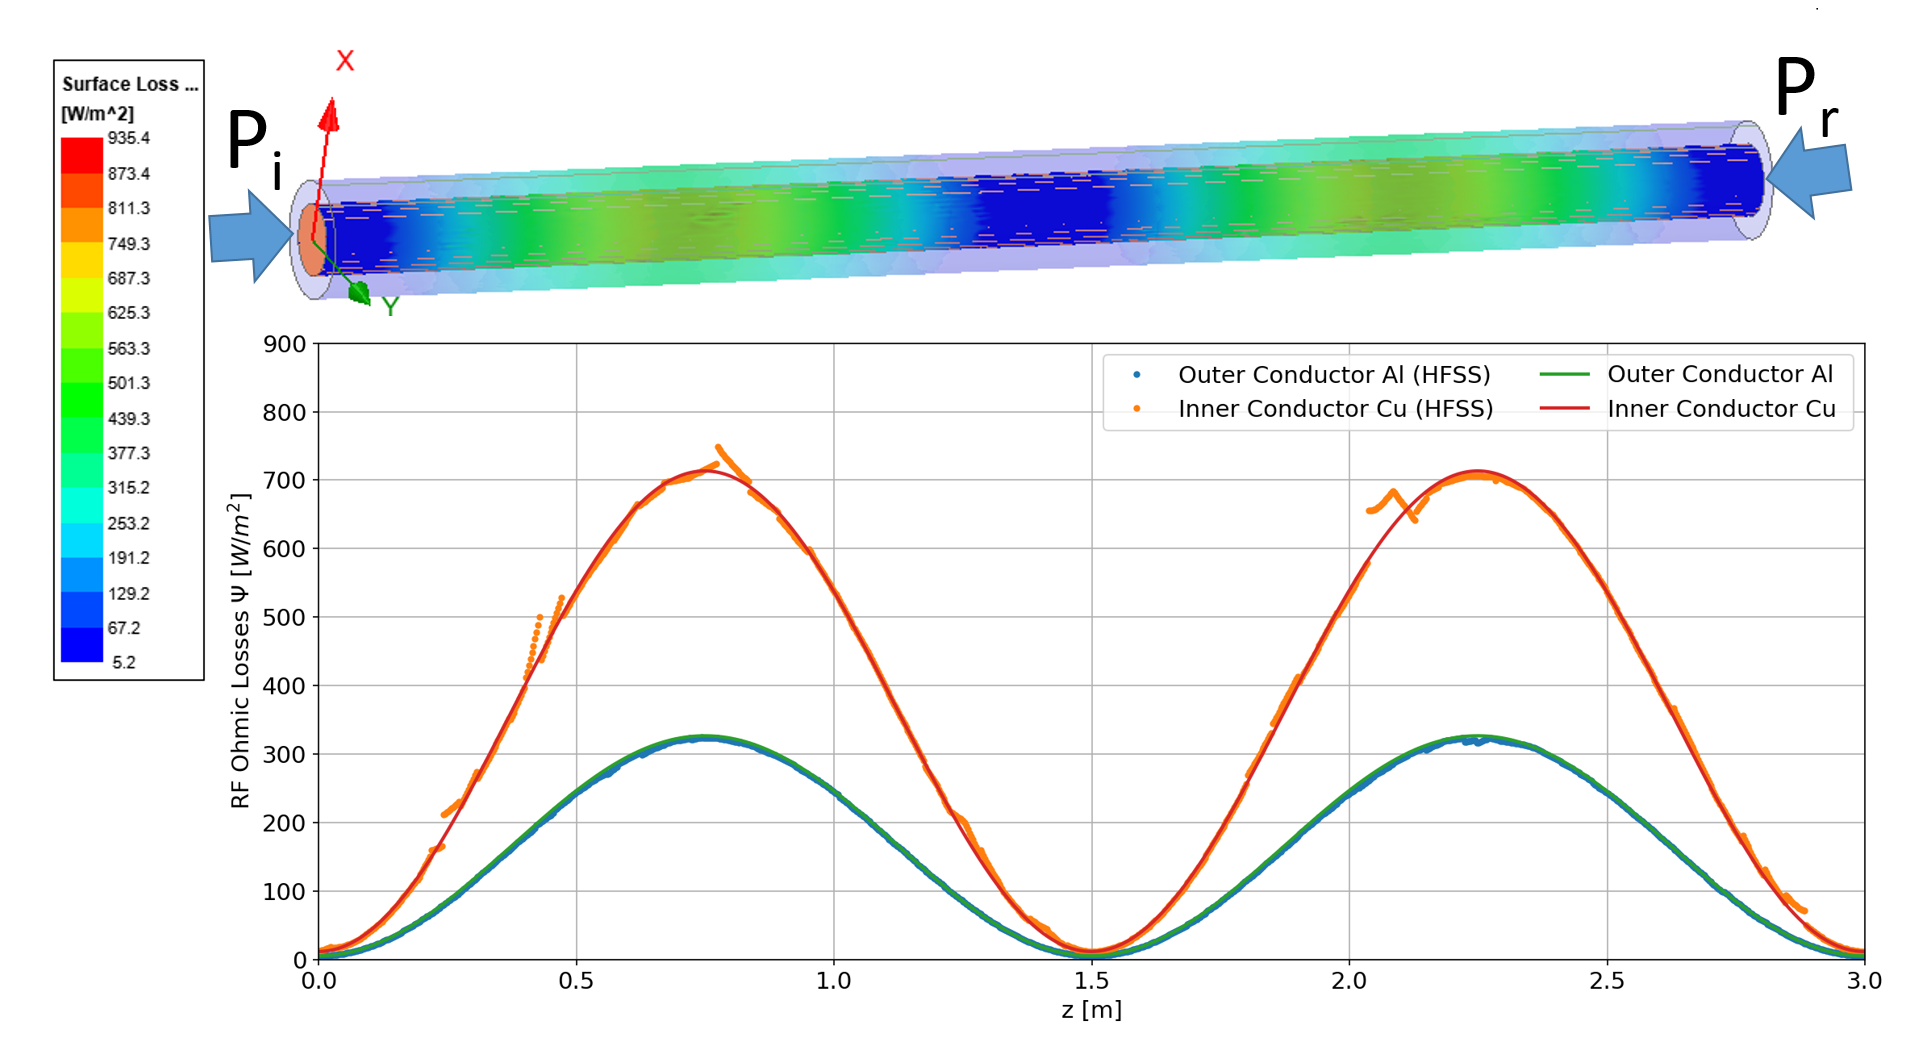
\includegraphics[width=1.0\linewidth]{figures/chap3/coaxial_losses}
	\caption{Coaxial losses in a 2~meter 30~\si{\Omega} 9" coaxial line with $P_\mathrm{i}=500~\si{kW}$ and  $P_\mathrm{r}=300~\si{kW}$ at 100~\si{MHz}. Inner conductor is in copper while the outer conductor is in aluminium. Heat flux from Eq.(\ref{eq:ohmic_heat_flux_coaxial}) is benchmarked against full-wave ANSYS HFSS.}
	\label{fig:coaxial_losses}
\end{figure}

%Finally, the attenuation $\alpha=P_\ell(z=0)/(2P_0)$ in $[\si{Neper/m}]$ of a coaxial line is\cite[Ex.2.7]{pozar2012}:
%\begin{equation}
%\alpha 
%	=
%	\frac{1}{4\pi Z_0}
%	\left(
%		\frac{R_{s,a}}{a} + \frac{R_{s,b}}{b}
%	\right)
%	+
%	\frac{1}{2}\omega \varepsilon'' \eta
%\end{equation}
%where $R_{s,a}$ and $R_{s,b}$ are the sheet resistances given by eq.\ref{eq:sheet_resistance} for inner and outer conductors respectively and $\eta=\sqrt{\mu/\varepsilon'}$ is the intrinsic impedance of the dielectric material filling the coaxial line. 

% #####################################################
% #####################################################
\section{Rectangular Waveguides}\label{sec:rectangular_waveguide}
\subsection{Rectangular Waveguides Main Properties}
Electromagnetic wave can also propagate in hollow metallic structures filled with dielectric. The structure dimensions must be designed to the wavelength to transport. Waveguides can support different kinds of modes, the most conventiannol being TE (Transvere Electric) and TM (Transverse Magnetic) modes. 

\begin{marginfigure}[0cm]
	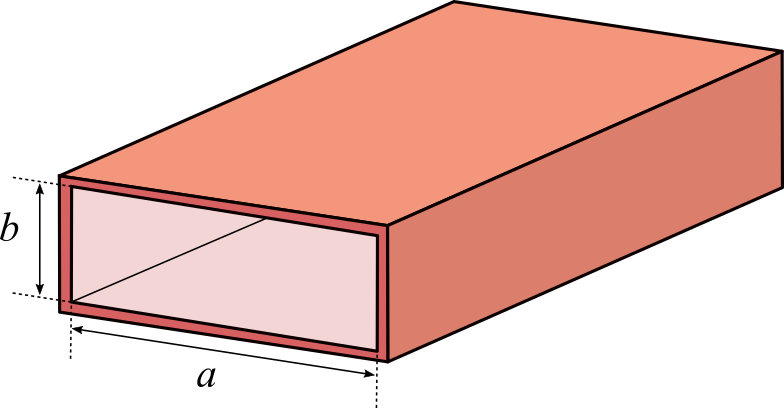
\includegraphics[width=1\linewidth]{figures/chap3/rectangular_waveguide}
	\caption{Rectangular Waveguide Geometry}
	\label{fig:rectangular_waveguide_geometry}
\end{marginfigure}

A hollow rectangular waveguide of width $a$ and height $b$ is illustrated in Figure \ref{fig:rectangular_waveguide_geometry}. Solving Maxwell’s equations for this geometry leads to multiple possible solutions, or \emph{modes}. In a rectangular waveguide, modes can be expressed as \emph{Transverse Electric} (TE) or \emph{Transverse Magnetic} (TM), depending of their respective polarization. Since the walls of a rectangular waveguide constrain the electromagnetic field boundary conditions along two dimensions, two integer indices $m$ and $n$ are used to describe a mode from another. Thus, modes in a rectangular waveguides can be $\TE_{mn}$ or $\TM_{mn}$\sidenote{With $m$ and $n$ integers greater or equal to 0 for $\TE$ modes and greater or equal to 1 for $\TM$ modes.}. These modes are eigenfunctions of the equation system and each mode is characterized by a wavenumber $\beta_{mn}$:
\begin{equation}
	\beta_{mn} = \sqrt{k^2_0 - k_{c,mn}^2 }
	\label{eq:rectwg_wavenumber}
\end{equation}
with $k_0=\omega\sqrt{\mu\varepsilon}=\sqrt{\mu_r \varepsilon_{r}}\omega/c$ and where $k_{c,mn}$ is the \textit{cut-off wavenumber}:
\marginnote{We recall here for convenience that the medium wavelength $\lambda$ is:
	$$
	\lambda = \frac{\lambda_0}{n} = \frac{v_\phi}{f}
	$$
	where $\lambda_0$ is the wavelength in vacuum, $v\phi$ is the phase velocity, $n=c/v_\phi=\sqrt{\mu_r \varepsilon_{r}}$ is the refractive index and $c=1/\sqrt{\mu_0 \varepsilon_{0}}$ the speed of light. We also define 
	$$
	\xi_0=\sqrt{\frac{\mu_0}{\varepsilon_{0}}}=120\pi=377\,\si{\Omega}
	$$ 
	as the vacuum characteristic impedance.
}
\begin{equation}
	k_{c,mn}
	=
	\sqrt{\left(\frac{m\pi}{a}\right)^{2}+\left(\frac{n\pi}{b}\right)^{2}}
	\label{eq:rectwg_cutoff_wavenumber}
\end{equation}

Each mode has an associated \textit{cut-off frequency} $f_{c,mn}$, below which a mode cannot propagate in the guide:
\begin{equation}
	f_{c,mn} = \frac{k_{c,mn}}{2\pi\sqrt{\mu \varepsilon}}
	\label{eq:rectwg_cutoff-frequency}
\end{equation}
The mode $mn$ can propagate in a rectangular waveguide only if the operating frequency is higher than the cut-off frequency of the mode, i.e. $f>f_{c,mn}$. The mode with the lowest cut-off frequency is called the \textit{fundamental} or \textit{dominant} mode. Because we have assumed that $a>b$, the lowest cut-off frequency occurs for the $\TE_{10}$ ($m=1,n=0$) mode\sidenote{There are no $\TE_{00}$ mode.}. 

For practical applications, the dimensions of the waveguides are generally chosen in order to have one and only one mode allowed propagating for a specified frequency band. Other modes can eventually be excited by waveguides discontinuities, but can’t propagate since they are evanescent ($k^2_0 < k_{c,mn}^2$ in Eq.(\ref{eq:rectwg_wavenumber})). Such modes are referred to \textit{high order modes}. For high power applications, a great care is given to waveguide inner walls, bends and connections, since reflected power and breakdowns may occur due to discontinuities in the conducting walls, such as the ones caused by flange misalignments \sidecite{harvey1955,brady1965,kerr2010}, bumps, holes, etc.

% #####################################################
\subsection{Electric and Magnetic Fields}
At a given frequency in a homogeneous-filled metallic hollow waveguide, the set of all possible TE and TM modes forms an orthogonal basis and a complete system\cite[§1.2]{marcuvitz1951},\cite[§5.2]{Collin1990},\cite[§8.2]{Harrington2001}. In practice, this sum is over all propagating modes and truncated to few evanescent modes only if needed, which is the case for antenna-plasma coupling calculations (Cf. Section~\ref{sec:lhcd}). In order to match the geometry usually used for plasma-wave coupling theory, we assume here that the large side of the waveguide is aligned in the direction $y$ and the short side in the direction of $z$. The waveguide cross-section is supposed homogenous in the $x$ direction. The geometry of a rectangular waveguide is illustrated in Fig.\ref{fig:rectangular_waveguide_geometry_fields}. The transverse electromagnetic fields can be expressed the summation of these modes:

\begin{marginfigure}[0cm]
	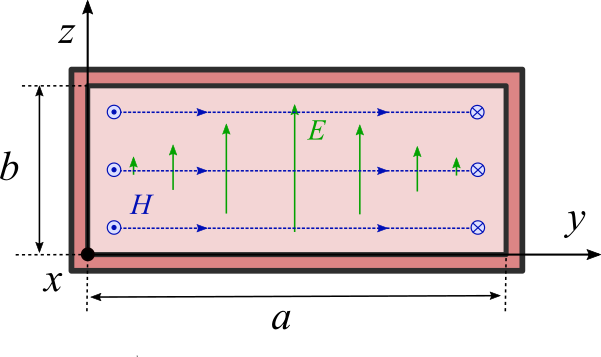
\includegraphics[width=1\linewidth]{figures/chap3/rectangular_waveguide_fields}
	\caption{Rectangular Waveguide Geometry and $\TE_{10}$ mode pattern derived from Eq.(\ref{eq:rectwg_EHfields_TE10})}
	\label{fig:rectangular_waveguide_geometry_fields}
\end{marginfigure}

\begin{subequations}
	\begin{align}
\mathbf{E}_{t}(\mathbf{r}) = & \sum_{p,m,n} V_{pmn}(x)\mathbf{e}_{pmn} (y,z)
\label{eq:E_guides_somme_modes}\\
\mathbf{H}_{t}(\mathbf{r}) = & \sum_{p,m,n} I_{pmn}(x)\mathbf{h}_{pmn} (y,z)
\label{eq:H_guides_somme_modes}
	\end{align}
\label{eq:rectwg_transverse_fields_sum_modes}
\end{subequations}
with $V_{pmn}$ and $I_{pmn}$ the eigenvalues of a mode $p=\{\TE,\TM\}$ of indexes $(m,n)$ and $\gamma_{pmn}=j\beta_{pmn}$ its associated wavenumber. 

\begin{subequations}
	\begin{align}
V_{pmn}(x) = & A_{pmn}e^{-\gamma_{pmn}x} + B_{pmn}e^{+\gamma_{pmn}x}
\label{eq:valeur_propre_V}\\
I_{pmn}(x) = & \frac{1}{Z_{pmn}}\left(A_{pmn}e^{-\gamma_{pmn}x} - B_{pmn}e^{+\gamma_{pmn}x}\right)
\label{eq:valeur_propre_I}
	\end{align}
	 \label{eq:rectwg_modes_eigenvalues}
\end{subequations}
with $Z_{pmn}$ the mode characteristic impedance:
\begin{equation}
Z_{pmn} = 
\begin{cases}
\frac{j\omega\mu}{\gamma_{mn}} = \frac{j k_0 \xi_0}{\gamma_{mn}} & \mathrm{\, for\, \TE\, modes}\\
\frac{\gamma_{mn}}{j\omega\varepsilon}=\frac{\gamma_{mn} \xi_0}{j k_0} & \mathrm{\, for\,\TM\, modes}
\end{cases}
\end{equation}

The model eingenfunction for rectangular waveguides are\cite[§2.2]{marcuvitz1951},\cite[§8.1,§8.2]{Harrington2001},\cite[§5.4]{Collin1990},\cite[§3.3]{pozar2012},\cite[Appendix A]{Bers1981} for TE modes:
\begin{eqnarray}
\mathbf{e}_{mn}^{\TE}(y,z) & = & -\ebf_x \times \mathbf{h}_{mn}^{\TE} = \ebf_x \times \nabla_{t} \psi_{mn}\\
\mathbf{h}_{mn}^{\TE}(y,z) & = &  \ebf_x \times \mathbf{e}_{mn}^{\TE} = -\nabla_{t} \psi_{mn}
\label{eq:TEmodes_eingenfunctions}
\end{eqnarray}
and mode TM modes:
\begin{eqnarray}
\mathbf{e}_{mn}^{\TM}(y,z) & = & -\nabla_{t}\phi_{mn}\\
\mathbf{h}_{mn}^{\TM}(y,z) & = & \ebf_x \times\mathbf{e}_{mn}^{\TM}= -\ebf_x \times\nabla_{t}\phi_{mn}
\label{eq:TMmodes_eingenfunctions}
\end{eqnarray}
The longitudinal components are given by:
\begin{eqnarray}
E_{x}^{TM} & = & \sum_{m,n}\frac{k_{c,mn}^{2}}{j k_{0}}\xi_0 I_{m,n}(x)\phi_{mn}(y,z)\\
H_{x}^{TE} & = & \sum_{m,n}\frac{k_{c,mn}^{2}}{j k_{0}}\xi_0^{-1} V_{m,n}(x)\psi_{mn}(y,z)
\label{eq:TETM_longitudinal_components}
\end{eqnarray}
$\psi$ and $\phi$ are the generator functions (\emph{transverses field pattern mode functions}). For a rectangular waveguide\cite[Table 8.1]{Harrington2001}\cite[§1.2 (6.c),§2.2]{marcuvitz1951}\cite[Appendix A, A13-14]{Bers1981}:
\begin{eqnarray}
\psi_{mn} & = & \frac{1}{\pi}\sqrt{\frac{\epsilon_{m}\epsilon_{n}}{m^{2}\frac{b}{a}+n^{2}\frac{a}{b}}}\cos\left(\frac{m\pi}{a}y\right)\cos\left(\frac{n\pi}{b}z\right)\label{eq:fonction_generatrice_TE}\\
\phi_{mn} & = & \frac{2}{\pi}\sqrt{\frac{1}{m^{2}\frac{b}{a}+n^{2}\frac{a}{b}}}\sin\left(\frac{m\pi}{a}y\right)\sin\left(\frac{n\pi}{b}z\right)\label{eq:fonction_generatrice_TM}
\end{eqnarray}
where $\epsilon_{k}=1$ if $k=0$ or $\epsilon_{k}=2$ otherwise.

Since these solutions form a orthogonal basis, the following integral over the waveguide cross-section $S$ gets\cite{marcuvitz1951,Collin1990}:

\begin{equation}
\left\langle \mathbf{f},\mathbf{g}\right\rangle 
=
\iint_{S}\mathbf{f}(y,z)\mathbf{\cdot g}(y,z)\, \diff y\, \diff z
\label{eq:rectwg_scalar_product}
\end{equation}
in particular:
\begin{subequations}\label{eq:relations_orthogonalite}
	\begin{eqnarray}
	\left\langle \mathbf{e}_{mn}^{\TE},\mathbf{e}_{m'n'}^{\TE}\right\rangle  & = & \delta_{m=m',n=n'}\\
	\left\langle \mathbf{e}_{mn}^{\TE},\mathbf{h}_{m'n'}^{\TE}\right\rangle  & = & \delta_{m=m',n=n'}\\
	\left\langle \mathbf{e}_{mn}^{\TE},\mathbf{e}_{m'n'}^{\TM}\right\rangle  & = & 0\\
	\left\langle \mathbf{e}_{mn}^{\TE},\mathbf{h}_{m'n'}^{\TM}\right\rangle  & = & 0
	\end{eqnarray}
\end{subequations}
where $\delta_{m=m',n=n'}=1$ if $m=m'$ and $n=n'$, $0$ otherwise.

For the fundamental mode $\TE_{10}$ (with $a>b$), one has in particular:
\begin{subequations}
	\begin{align}
\psi_{10}(y) &= 
	\frac{1}{\pi} \sqrt{\frac{2a}{b}} \cos\left(\frac{\pi}{a} y\right) 
	\\
\Ebf_t(x,y) =& 
	-  \sqrt{\frac{2}{ab}} \sin\left(\frac{\pi}{a} y\right)V_{10}(x) \hat\ebf_z 
	\\
\Hbf_t(x,y) =& 
	   \sqrt{\frac{2}{ab}} \sin\left(\frac{\pi}{a} y\right)I_{10}(x)\hat\ebf_y 
	\\
H_x(x,y) =& 
	\frac{k_{c,10}^2}{j \omega\mu} \frac{1}{\pi} \sqrt{\frac{2a}{b}} \cos\left(\frac{\pi}{a} y\right) V_{10}(x)
	\end{align}
	\label{eq:rectwg_EHfields_TE10}
\end{subequations}
\marginnote[-3cm]{We we have used $\omega\mu=k_0\xi_0=\beta_{mn}Z_{mn}$.}

% #####################################################
\subsection{Power and Losses}
The previous choice of normalization factors leads to simple time-average power flow along a rectangular waveguide:
\begin{equation}
P=\iint\frac{1}{2}\Re\left[\mathbf{E}_{t}\times\mathbf{H}_{t}^{*}\right]\cdot \hat \ebf_x \diff S
=
\sum_{l}\frac{1}{2Z_{l}}\left(\left|A_{l}\right|^{2}-\left|B_{l}\right|^{2}\right)
\label{eq:poynting}
\end{equation}
where the sum is over the propagating modes only. 

Since the $\TE_{10}$ mode is the fundamental mode and the most used to transfer the RF power, we will specify some quantities for $m=1,n=0$. Using Eqs.(\ref{eq:rectwg_EHfields_TE10}), the power flow down the guide for the $\TE_{10}$ is:
\begin{equation}
	P_{10} = \frac{1}{2} \Re \iint_S  \left(\Ebf \times \Hbf^* \right)\cdot \hat\ebf_x \diff y \diff z
	= \frac{1}{2} \Re\left[V_{10}(x) I^*_{10}(x) \right]
	\label{eq:rectwg_poynting_TE10_V10_I10}
\end{equation}
which reads from Eqs.(\ref{eq:rectwg_modes_eigenvalues}):
\begin{equation}
	P_{10} = \frac{1}{2Z_{10}}\left(\left|A_{10}\right|^{2}-\left|B_{10}\right|^{2}\right)
	\label{eq:rectwg_poynting_TE10_A10_B10} = P_\mathrm{i} -  P_\mathrm{r}
\end{equation}
where $P_\mathrm{i}$ (in [\si{W}]) is the forward power and $P_\mathrm{r}$ the reflected power. Coefficients $|A_{10}|$ and $|B_{10}|$ can then be related conveniently to the forward and reflected power:
\begin{subequations}
	\begin{align}
	|A_{10}| =& \sqrt{2Z_{10} P_\mathrm{i}} \\
	|B_{10}| =& \sqrt{2Z_{10} P_\mathrm{r}} =  R |A_{10}|
	\end{align}	
\end{subequations}	
where we have used the "voltage" reflection coefficient $R$ defined by $R^2=P_\mathrm{r}/P_\mathrm{i}$. Using all the previous definitions, the electromagnetic field in Eqs.(\ref{eq:rectwg_EHfields_TE10}) can be directly related to forward and reflected powers, giving peak values comparable to full-wave calculations and for breakdown analysis. A simple benchmark of these relations is given on Fig.\ref{fig:rectwg_benchmark_fields}.

The electric field for the $\TE_{10}$ mode is maximum at $x=a/2$ (in the middle of the waveguide). This peak electric field value for this mode is:
\begin{equation}
	\left| E_{y,\mathrm{max}} \right|
	=
	2 \sqrt{\frac{Z_{10} P_\mathrm{i}}{a b }} 
		\left( 
			1 + R
		\right)
\end{equation}

The maximum incident power before breakdown for a given reflection coefficient in a dielectric-filled rectangular waveguide is thus:
\begin{equation}
	P_{\mathrm{max,bd}}
	= 
	\frac{a b}{4 Z_{10}} \frac{E_d^2}{\left(1 + R\right)^2}
\end{equation}
with $E_d$ the electric strength of the medium. The previous expression shows that the maximum power is again obtained for a minimum reflection coefficient and increase with the waveguide dimensions. 

The Ohmic loss is not homogeneous in a rectangular waveguide. The Ohmic power loss density (in [$\si{W/m^2}$]) is, for the large ($\Psi_a$) and the small ($\Psi_b$) sides of the waveguide respectively:
\begin{subequations}
	\begin{align}
		\Psi_a(x,y)
		=& \frac{R_s}{2} \left(\left| H_x(x,y) \right|^2 + \left| H_y(x,y) \right|^2 \right)
\\
		\Psi_b(x)
		=& \frac{R_s}{2} \left| H_x(x,0) \right|^2 
	\end{align}
\end{subequations}

From symmetry, the currents on the top and bottom walls are identical, as are the currents on the small walls. So, the Ohmic power loss per unit length $P_\ell$ (in \si{W/m}) for a waveguide is then: 
\begin{equation}
P_\ell (z)
= 
2\int_0^a  \Psi_a(x,z) \diff x 
+ 
2\int_0^b  \Psi_b(z) \diff y 
\end{equation}
which reads:
\begin{equation}
P_\ell (z)
= 
R_s \left[
	\frac{1}{b} \left| I_{10} \right|^2 
	+ 
	\left(
		2a + \frac{a^2}{b}
	\right)
	\frac{k_{c,10}^2}{(\omega\mu\pi)^2} 
	\left| V_{10} \right|^2 
\right]
\label{eq:rectwg_power_loss_per_unit_length}
\end{equation}

\begin{figure}
	\centering
	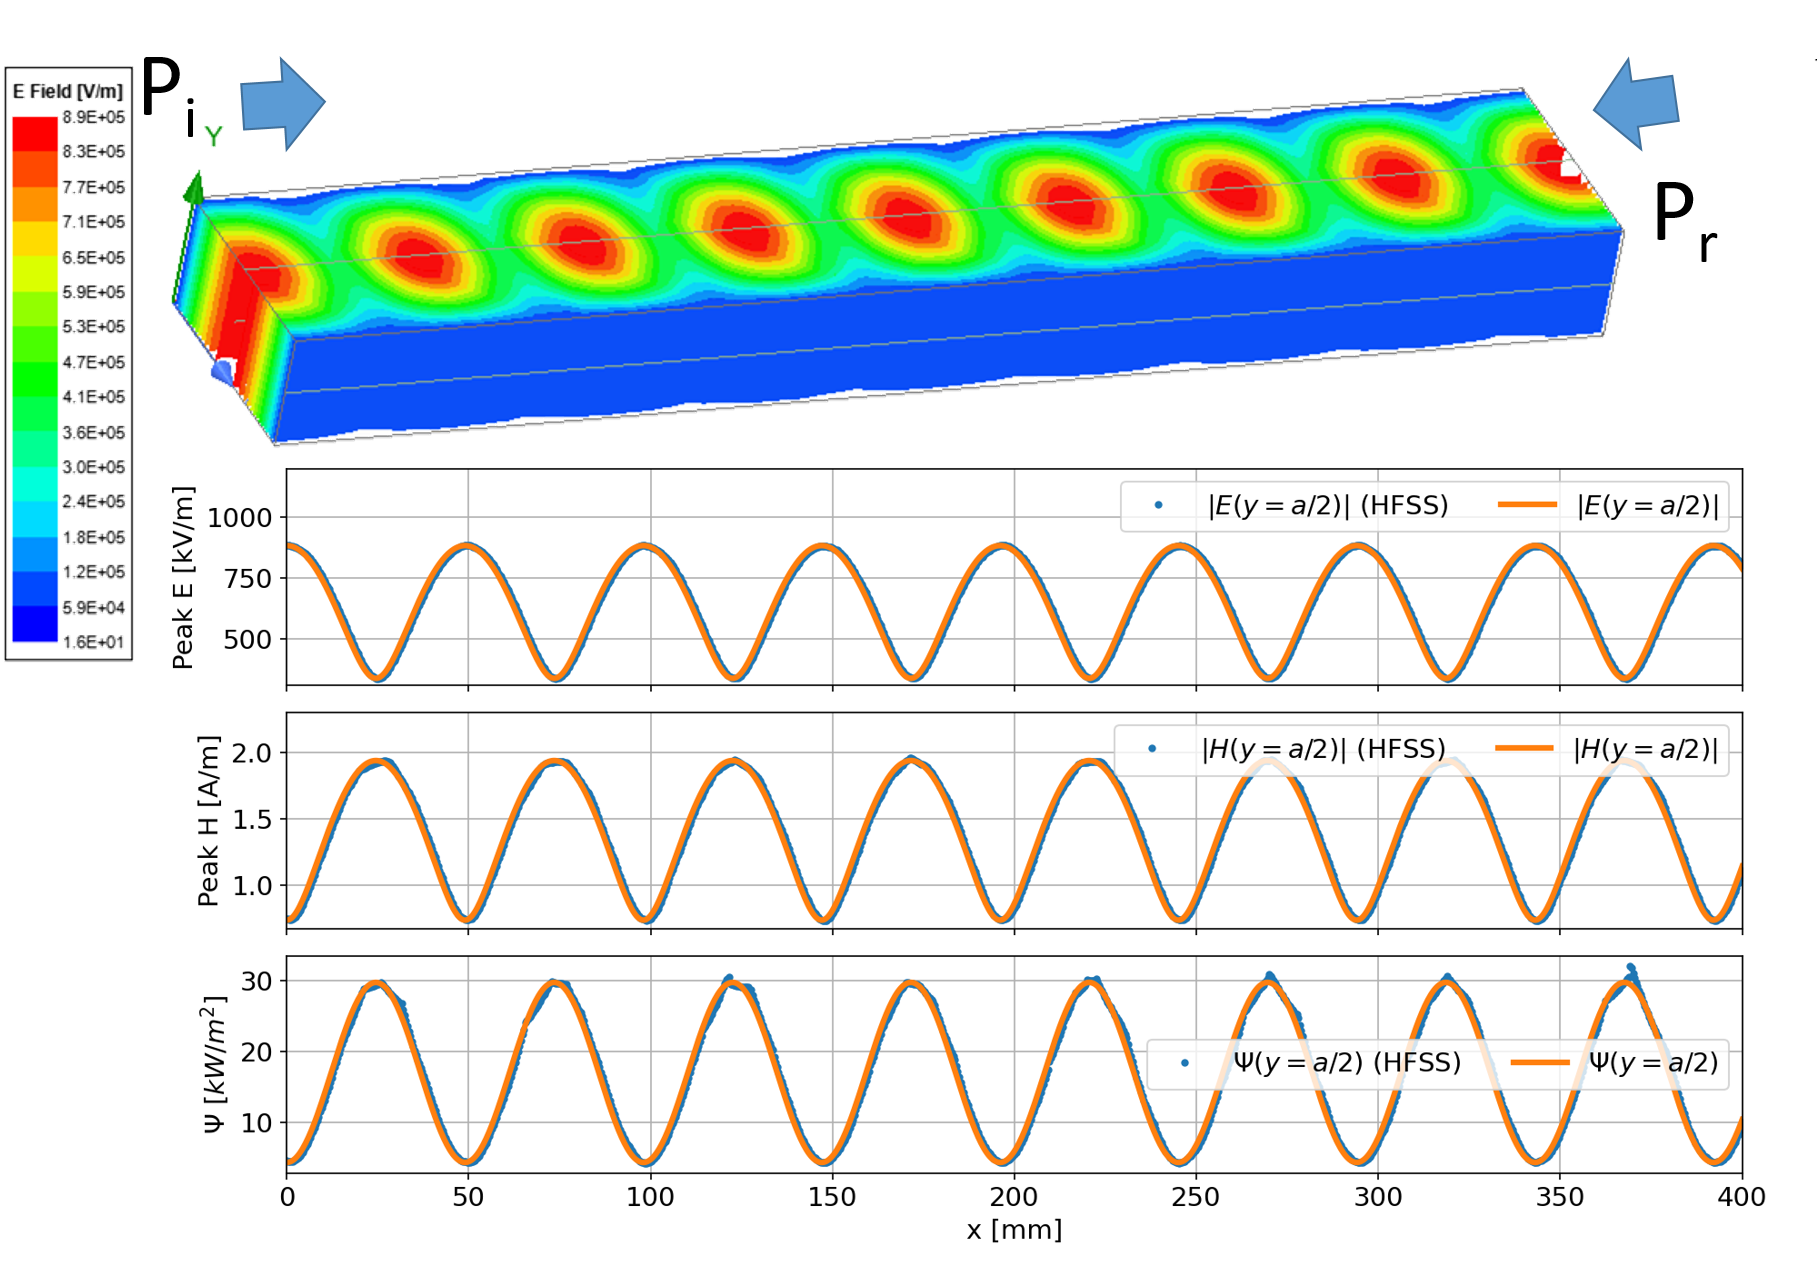
\includegraphics[width=1.0\linewidth]{figures/chap3/rectangular_waveguide_fields_losses}
	\caption{$E$ and $H$ fields and RF losses in a 400~\si{mm} WR284 waveguide ($72.13 \times 34.04$~\si{mm}) with $P_\mathrm{i}=500~\si{kW}$ and  $P_\mathrm{r}=100~\si{kW}$ at 3.7~\si{GHz}. Conductor are in copper. Results are  benchmarked against full-wave ANSYS HFSS.}
	\label{fig:rectwg_benchmark_fields}
\end{figure}



	
	% RF Coupling
	% RF coupling
\setchapterimage{figures/chap2/chapter_head} % Optionally specify theheight
\setchapterpreamble[u]{\margintoc}
\chapter{RF Coupling}
\label{chap:rf_coupling}


This chapter aims to give the key elements in order to derive the optimum characteristics for RF plasma heating or current drive antennas. The section \ref{sec:waves-in-plasma} recall the necessary elements to characterize the propagation medium, in particular the kind of cold plasma wave modes that can propagate in the plasma as a response to a given RF excitation. The sections \ref{sec:icrh} and \ref{sec:lhcd} focuses on the specific ICRH and LHCD range of frequencies. 

Many antenna-plasma coupling models have been developed and most rely on a "slab" approximation which consists in assuming uniformity in the toroidal and poloidal directions while imposing a radiation boundary condition in the radial direction. While much of the essential physics of the coupling at the plasma–antenna interface can be elucidated using this slab approximation, real-life experiments presents additional problems since plasma is not homogeneous, antenna geometries can be complex, images currents are induced on the passive conducting elements surrounding the antenna and antennas excitation is not perfect. Thus, plasma response and wave fields must be solved with more refinements, treating the antenna geometry as accurately as possible. Antenna-plasma coupling is still a topic of continued research interest and some contributions are presented in Section~\ref{sec:ALOHA}, \ref{sec:LHCD_FW_antena_coupling} and \ref{sec:ICRH_FW_antena_coupling}.


\section{RF Waves In Plasma}\label{sec:waves-in-plasma}
This section is a reminder of the basic properties of wave propagation in a magnetized plasma. In-depth treatment and derivations of the results given in this section can be found in the standards physics oriented textbooks \sidecite{stix1992, Brambilla1998, Swanson2003, Cairns1991, Golant1989}. 

\subsection{Maxwell Equations in Time Harmonic Regime}
We shall start the Maxwell equations in terms of vector fields in three dimensions, before recasting them to fit our needs. The usual electromagnetic field quantities are expressed following the terminology used in \citeauthyear{Harrington2001}:
\begin{itemize}
	\item $\boldsymbol{\mathcal{E}}$: the electric field intensity (in $\si{V/m}$)
	\item $\boldsymbol{\mathcal{H}}$: the magnetic field intensity (in $\si{A/m}$)
	\item $\boldsymbol{\mathcal{D}}$: the electric flux density (in $\si{A.s/m^2=C/m^2}$)
	\item $\boldsymbol{\mathcal{B}}$: the magnetic flux density (in $\si{V.s/m^2} = \si{Wb/m^2} := \si{T}$)
	\item $\boldsymbol{\mathcal{J}}$: the electric current density (in $\si{A/m^2}$)
	\item $q_v$: the electric charge density (in $\si{C/m^3}$)
\end{itemize}
where all quantities are function of space and time, e.g. $\boldsymbol{\mathcal{E}}=\boldsymbol{\mathcal{E}}(\mathbf{r},t)$. Maxwell equations can be stated as:
\begin{subequations}
	\begin{align}
		\boldsymbol{\nabla} \times \boldsymbol{\mathcal{E}} &= -\frac{\partial \boldsymbol{\mathcal{B}}}{\partial t} \label{eq:Maxwell-Faraday}\\
		\boldsymbol{\nabla} \times \boldsymbol{\mathcal{H}} &= \frac{\partial \boldsymbol{\mathcal{D}}}{\partial t} + \boldsymbol{\mathcal{J}} \label{eq:Maxwell-Ampere} \\
		\boldsymbol{\nabla} \cdot \boldsymbol{\mathcal{D}} &= q_v \label{eq:Maxwell-Gauss} \\
		\boldsymbol{\nabla} \cdot \boldsymbol{\mathcal{B}} &= 0 \label{eq:Maxwell-Gauss-Magnetism}
	\end{align}
	\label{eq:MaxwellEquations}
\end{subequations} 


The previous expressions are non-linear by nature. In order to make further understanding of the plasma waves, we will limit our analysis to a stationary and an homogeneous plasma. Moreover, we will assume that Radio-Frequency source time excitation varies sinusoidally in time with a single frequency. Such case of time varying electromagnetic fields is referred as time-harmonic  \sidecite{Harrington2001} and the analysis of fields quantities $\boldsymbol{\mathcal{A}}$ can be simplified by using complex quantities $\Abf$\footnote{The choice of the time sign convention $+j\omega t$ is motivated to match the one adopted in most RF solvers, commercial or the ones developed in this work, which is most prevalent in electrical engineering texts. Note that in general, waves in plasma texts use the opposite sign convention, ie. $e^{-i\omega t}$\cite{bradley2007, michelsen2019}. While both conventions are mathematically valid, the use of $exp(–j\omega t)$ can be preferable when dealing with the principal value of complex number square roots, which does not require numerical tricks as the ones defined for example in \cite{Hillairet2007a}. Using $j=-i$ allows one to convert results from one convention to the other.}:
\marginnote{We will adopt $j$ as the complex unit, ie. $j^2=-1$.}
\begin{equation}
\boldsymbol{\mathcal{A}}(\rbf,t) 
	\stackrel{\Delta}{=} 
	\left| \Abf(\rbf) \right| \cos\left(\omega t + \phi \right) 
	= 
	\Re \left[ \Abf(\rbf) e^{j\omega t} \right]
\end{equation}
\marginnote{This solution can be generalized to finite bandwidth cases, which are a continuous distribution of frequencies $\omega$, by defining the field as summation of time-harmonic solutions over all frequencies: 
$$
\boldsymbol{\mathcal{A}}(\rbf,t) 
	\stackrel{\Delta}{=} 
	 \int  \Re\left[\boldsymbol{\mathcal{A}}(\rbf,\omega)e^{j\omega t}  \diff \omega \right]
$$
which can be seen as a time-domain Fourier transform. Moreover, since $\boldsymbol{\mathcal{A}}(\rbf,t) $ is real function, then $\boldsymbol{\mathcal{A}}(\rbf,-\omega)=\boldsymbol{\mathcal{A}}^*(\rbf,\omega)$ by property of the Fourier transform.}
To simplify the mathematical treatment, it is convenient to represent field phasors $\Abf(\mathbf{r})$ in the Fourier space using a plane-wave expansion \sidecite[+5cm]{clemmow1996}: 
\begin{equation}
		\boldsymbol{\mathcal{A}}(\mathbf{r}, t) 
		=
		\Re \left[
		\int 
		\mathbf{A}(\kbf) e^{j(\omega t - \kbf\cdot\rbf)}
		\diff \kbf \;
		\right]
	\label{eq:k-spectralDefinition}
\end{equation}
where each plane wave is characterized by their wavevector $\kbf=(k_x, k_y, k_z)$. 

Plugging such a solution into the Maxwell equations (\ref{eq:MaxwellEquations}) leads to algebraic equations:
\begin{subequations}
	\begin{align}
		\kbf \times \Ebf (\kbf) 
		=& 
		\omega \Bbf (\kbf)
		\\
		\kbf \times \Hbf (\kbf) 
		=& 
		-\omega \Dbf (\kbf)
		+ 	
		j\Jbf (\kbf) 
		\\
		\kbf  \cdot \Dbf (\kbf) 
		=& j q_v(\kbf) 
		\\
		\kbf  \cdot \Bbf (\kbf) 
		=& 0
	\end{align}
	\label{eq:k-omegaMaxwellEquations}
\end{subequations}

% ###########################################################################
% ###########################################################################
\subsection{Constitutive Relations}
Fluxes densities $(\boldsymbol{\mathcal{D}}, \boldsymbol{\mathcal{B}})$ differ from field intensities $(\boldsymbol{\mathcal{E}}, \boldsymbol{\mathcal{H}})$ inside materials with regards to their relative magnitude and direction. Flux densities can be interpreted  as a response of the medium to an applied excitation. One can thus express $(\boldsymbol{\mathcal{D}},\boldsymbol{\mathcal{B}})$ and $\boldsymbol{\mathcal{J}}$ in terms of $(\boldsymbol{\mathcal{E}},\boldsymbol{\mathcal{H}})$, also known as the constitutive relationships written in the most general form as\sidecite{Harrington2001}:
\begin{subequations}
	\begin{align}
		\boldsymbol{\mathcal{D}} =& \boldsymbol{\mathcal{D}}(\boldsymbol{\mathcal{E}},\boldsymbol{\mathcal{H}}) \\
		\boldsymbol{\mathcal{B}} =& \boldsymbol{\mathcal{B}}(\boldsymbol{\mathcal{E}},\boldsymbol{\mathcal{H}}) \\
		\boldsymbol{\mathcal{J}} =& \boldsymbol{\mathcal{J}}(\boldsymbol{\mathcal{E}},\boldsymbol{\mathcal{H}})
	\end{align}
\end{subequations}
Some situations may arise where the induction fields are no more linearly proportional to the primitive intensity fields. In such cases, one needs to extend the definition of linearity using linear differential relations such as \sidecite{Mackay2010}:
\begin{subequations}
	\begin{align}
		\boldsymbol{\mathcal{D}} &= \varepsilon \boldsymbol{\mathcal{E}} + \varepsilon_1 \boldsymbol{\mathcal{E}}^2  + \ldots \\
		\boldsymbol{\mathcal{B}} &= \varepsilon \boldsymbol{\mathcal{H}} + \varepsilon_1 \boldsymbol{\mathcal{H}}^2 + \ldots \\
	\end{align}
\end{subequations}%
Such situation arises typically when high intensity RF fields are used, which leads to non-linear phenomenons such \emph{ponderomotive effect}~\sidecite[-1cm]{fukuyama1980, krapchev1981, theilhaber1982}, an effect studied for LHCD in \sidecite{preynas2013}.



A magnetized plasma can be considered as an anisotropic medium for electromagnetic waves \sidecite{stix1992}. In such case, the response of the medium is different depending on the polarization of the oscillating field and expressed by tensor constitutive relationships. Since we have assumed that the plasma is homogeneous and stationary, constitutive relations become algebraic time-invariant relationships \sidecite[-1cm]{Dumont2017}\marginnote{We will admit the generalized Ohm's law $\Jbf(\Ebf)=\sigma\Ebf$.}:
\begin{subequations}
	\begin{align}
		\Dbf(\kbf, \omega) 
		=& 
		\boldsymbol{\varepsilon}(\kbf, \omega) \cdot \Ebf(\kbf, \omega) 
		\label{eq:disp_relation_kw_D}
		\\
		\Bbf(\kbf, \omega) 
		=& 
		\boldsymbol{\mu}(\kbf, \omega) \cdot \Hbf(\kbf, \omega) 
		\label{eq:disp_relation_kw_B}
		\\
		\Jbf(\kbf, \omega) 
		=& 
		\boldsymbol{\sigma}(\kbf, \omega) \cdot \Ebf(\kbf, \omega) 
		\label{eq:disp_relation_kw_J}
	\end{align}
	\label{eq:k-omegaDispersionRelation}
\end{subequations}%
where $\boldsymbol{\varepsilon}$, $\boldsymbol{\mu}$ and $\boldsymbol{\sigma}$ are the dielectric, the permeability and the conductivity tensors respectively, which can be interpreted as 3x3 matrices \sidecite{Swanson2003}. We also define $\mu_0=4\pi\times10^7~\si{H/m}$ the vacuum magnetic permeability and $\varepsilon_0=1/(\mu_0 c^2)~\si{F/m}$ the vacuum dielectric permittivity with $c$ the speed of light. With the supplementary assumption that the medium is non-magnetic (i.e. $\boldsymbol{\mu}=\mu_0$), Maxwell equations (\ref{eq:k-omegaMaxwellEquations}) reads\marginnote{The $(\kbf,\omega)$ dependence is assumed implicitly from now for the ease of reading.}:
\begin{subequations}
	\begin{align}
		\kbf \times \Ebf  
		=& 
		\omega \mu_0 \Hbf
		\\
		\kbf \times \Hbf 
		=& 
		\left(
		-\omega \boldsymbol{\varepsilon} 
		+ 	
		j\boldsymbol{\sigma} 
		\right) \cdot 
		\Ebf
		\\
		\kbf  \cdot \boldsymbol{\varepsilon}  \cdot \Ebf 
		=& jq_v
		\\
		\kbf  \cdot \Hbf 
		=& 0	
	\end{align}
	\label{eq:maxwell_equations_kspace}
\end{subequations}

Combining the first two equations leads to the wave equation:
\begin{equation}
\kbf \times \kbf \times \Ebf + k_0^2 \Kbf \cdot \Ebf = 0
\label{eq:wave_equation_kxkxE}
\end{equation}
where $\Kbf$ the plasma equivalent permittivity tensor:
\begin{equation}
\Kbf(\omega) =  
\boldsymbol{\varepsilon}_r - \frac{j}{\omega \varepsilon_0} \boldsymbol{\sigma}
=
\left(
\begin{array}{ccc}
K_{xx} & K_{xy} & K_{xz} \\
K_{yx} & K_{yy} & K_{yz} \\
K_{zx} & K_{zy} & K_{zz} \\
\end{array}
\right)
\end{equation}  
Introducing the refraction index $\nbf = \kbf / \norm{\kbf} = \kbf/k_0$ leads to its normalized version:
\begin{equation}
\nbf \times \nbf \times \Ebf + \Kbf \cdot \Ebf = 0
\label{eq:wave_equation_nxnxE}
\end{equation}



% ############################################################
\subsection{Vacuum Dispersion Relation}
In a non-dispersive isotropic homogeneous non-lossy dielectric medium, such as vacuum (or air), the wavevector $\kbf$ direction is given from Eqs.(\ref{eq:maxwell_equations_kspace}):
\begin{equation}
\mathbf{\hat{k}}\cdot\mathbf{E}=0
\;\;\;\;\;\;
\mathbf{H}=\frac{n}{Z_{0}}\hat{\kbf}\times\mathbf{E}\label{eq:vecteur_onde_vide}
\end{equation}
where $n=\sqrt{\varepsilon_{r}}$ is the medium optical index. $Z_{0}=\sqrt{\frac{\mu_{0}}{\varepsilon_{0}}}=\mu_{0}c_{0}=\frac{1}{\varepsilon_{0}c_{0}}$ is the \emph{vacuum characteristic impedance}. The wave equation Eq.(\ref{eq:wave_equation_kxkxE}) can be put under matrix form:
\begin{equation}
\mathbf{M}(\kbf, \omega) \cdot \Ebf = 0
\end{equation}
which is a system of 3 equations and 3 unknowns $(E_{x},E_{y},E_{z})$. The condition for this system to have a non-trivial solution is equivalent to solving:
\begin{equation}
\det\left[\mathbf{M}(\kbf, \omega)\right] =  0
\end{equation}
which leads to a relationship between the wavevector $\kbf$ and the angular RF frequency $\omega$, called the \textit{dispersion relation} of the medium \cite[§4]{rothwell2018})\sidenote{While in a lossy medium $k^{2}=\mu\varepsilon\omega^{2}-j\omega\mu\sigma$ where $\sigma$ is the medium electrical conductivity in \si{S/m}.}. This relationship is simple for homogeneous dielectric medium:
\begin{equation}
k = \sqrt{\mu\varepsilon}\omega = n \frac{\omega}{c}
\end{equation}


% #################################################
% #################################################
\subsection{Cold Plasma Approximation}
In the so-called \textit{cold plasma} approximation, the temperature $T_s$ of all species $s$ in the plasma is supposed to be zero \cite[chap.5]{Brambilla1998}. Although this approximation seems restrictive, the cold plasma model describes surprisingly well the wave propagation in tokamak magnetized plasma. Such medium can support various kinds of waves, which main properties are derived in this section. 
\begin{marginfigure}
	\centering
	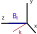
\includegraphics[width=0.8\linewidth]{figures/chap2/plasma-waves_geometry}
	\caption{Stix frame $(\mathbf{x},\mathbf{y},\mathbf{z})$, where $\mathbf{z}$ is in the direction of anisotropy (the direction of the magnetic field $\Bbf_0$). As plasma parameters are supposed invariant in the $\mathbf{y}$ direction (slab model), the wavevector $\kbf$ is in the $(\mathbf{x},\mathbf{z})$ plane. }
	\label{fig:plasma-wavesgeometry}
\end{marginfigure}
We follow the usual choice of geometry and coordinates illustrated in Figure~\ref{fig:plasma-wavesgeometry}, in which the $\mathbf{z}$ direction is taken along the direction of the magnetic field $\Bbf_0$.  The equivalent dielectric tensor in this frame can be written as the following form \sidecite[-3cm]{stix1992}:
\begin{equation}
\Kbf(\omega)
=
\left(\begin{array}{ccc}
	S & j D & 0\\
	-j D & S & 0\\
	0 & 0 & P
\end{array}\right)
\label{eq:stix_K}
\end{equation}
where
\begin{subequations}
	\begin{eqnarray}
	S(\omega) 
	& = & 
	1-\sum_{s}\frac{\omega_{i}^{2}}{\omega^{2}-\Omega_{s}^{2}}
	\label{eq:stix_S}
	\\
	D(\omega) 
	& = & 
	\sum_{s}\frac{\Omega_{s}}{\omega}\frac{\omega_{s}^{2}}{\omega^{2}-\Omega_{s}^{2}}
	\label{eq:stix_D}
	\\
	P(\omega) 
	& = & 
	1-\sum_{s}\frac{\omega_{s}^{2}}{\omega^{2}}
	\label{eq:stix_P}
	\end{eqnarray}
	\label{eq:stix_SDP}
\end{subequations}
where $\omega$, $\Omega_{s}$ and $\omega_{s}$ are respectively the RF, the \href{http://docs.plasmapy.org/en/v0.1/api/plasmapy.physics.parameters.gyrofrequency.html}{cyclotron} and the \href{http://docs.plasmapy.org/en/v0.1/api/plasmapy.physics.parameters.plasma_frequency.html#plasmapy.physics.parameters.plasma_frequency}{plasma} angular frequencies of the species $s$, defined by:
%\marginnote{The spatial dependence of the cyclotron and plasma frequencies come from density $n$ and magnetic field $B_0$ which can vary in space. }
\begin{subequations}
	\begin{eqnarray}
	\Omega_{s}  &=& Z\, e \frac{B_{0}}{m_{s}}
	\label{eq:cyclotron_angular_frequency} 
	\\
	\omega_{s}  &=& \sqrt{ \frac{Z^2 e^2 n_{s}}{\varepsilon_{0} m_{s}}}
	\end{eqnarray}
\end{subequations}
where $n_s$ is the density, $m_s$ the mass, $e$ the (signed) elementary charge and $Z$ the atomic number (number of protons) for the species $s$ (electron or ions). The parameters $S$, $D$ and $P$ depend of the plasma species densities and the magnetic field. Their values are illustrated in Figure~:\ref{fig:sdpvsfnfixedbfixed} for a Deuterium plasma for density and magnetic field representative of the one we could find in front of a Tore Supra/WEST antenna.

\begin{figure*}[h]
	\centering
	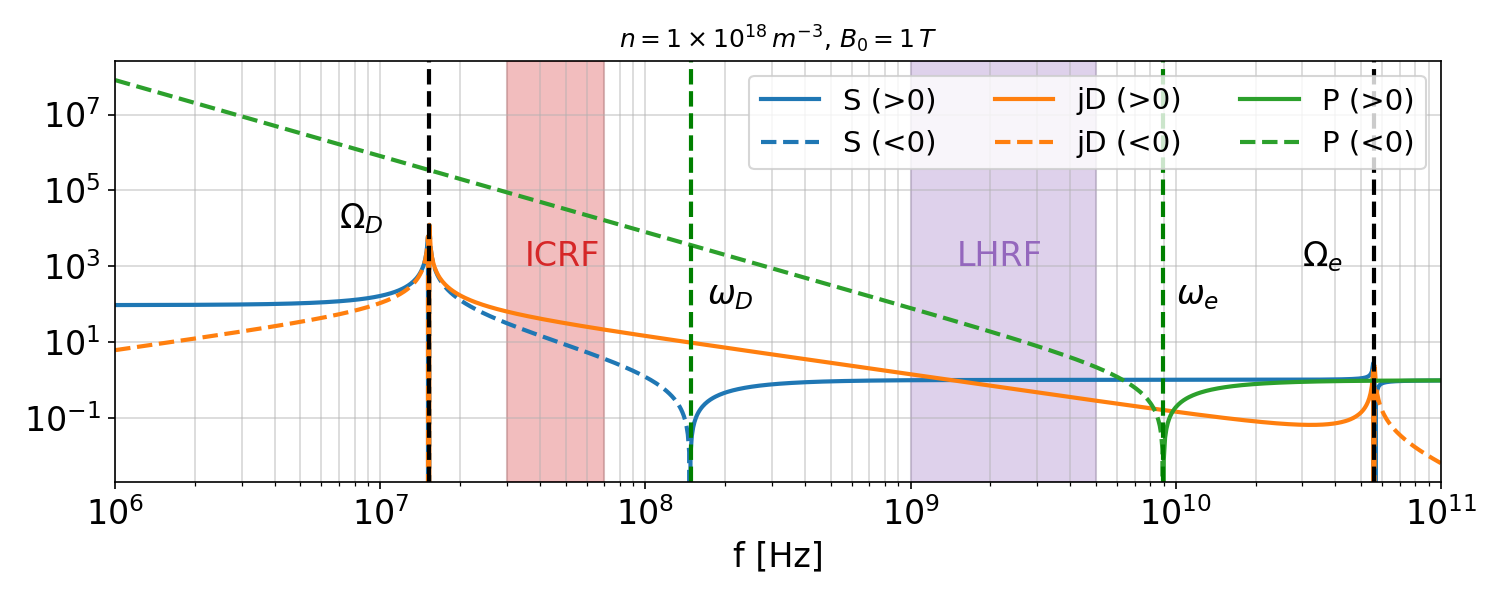
\includegraphics[width=1.0\linewidth]{figures/chap2/SDP_vs_f_nfixed_Bfixed}
	\caption{Values of the $S$, $D$, $P$ for a Deuterium plasma for density and magnetic field representative of the one we could find in front of a Tore Supra/WEST antenna. The typical Ion Cyclotron and Lower Hybrid range  of frequencies are indicated for convenience.}
	\label{fig:sdpvsfnfixedbfixed}
\end{figure*}

The form of Eq.(\ref{eq:stix_K}) is a consequence of the fact that the cold plasma is a gyrotropic media. Gyrotropic media are characterized by their invariance under any rotation about the direction of anisotropy~\cite{Mackay2010}, in our case the direction of the magnetic field $\Bbf_0/B_0=\mathbf{z}$. Hence, this tensor can be equivalently re-expressed into a rotation frame $(\mathbf{u}_{+}, \mathbf{u}_{-},  \mathbf{z})$, with $\mathbf{u}_{\pm}=(\mathbf{x}\pm \mathbf{y})/\sqrt{2}$:  
\begin{equation}
\Kbf(\omega)
=
\left(\begin{array}{ccc}
R & 0 & 0\\
0 & L & 0\\
0 & 0 & P
\end{array}\right)
\label{eq:stix_K_RLP}
\end{equation}
where $R$ is the \textit{right-hand} polarized component and $L$ is the \textit{left-hand} polarized component, defined as:
\marginnote{And inversely:, 
	$$
	S =  \frac{1}{2}\left(R+L\right)
	$$ 
	$$ 
	D = \frac{1}{2}\left(R-L\right)
	$$
Letters $S$, $D$, and $P$ originally come from \textit{sum}, \textit{difference} and \textit{plasma} terms \cite{stix1992}.}
\begin{subequations}
	\begin{eqnarray}
	R(\omega) 
	& = S + D = & 
	1-\sum_{s}\frac{\omega_{s}^{2}}{\omega(\omega+\Omega_{s})}
	\label{eq:stix_R}
	\\
	L(\omega)
	& = S - D = & 
	1-\sum_{s}\frac{\omega_{s}^{2}}{\omega(\omega-\Omega_{s})}
	\label{eq:stix_L}
	\end{eqnarray}
	\label{eq:stix_RL}
\end{subequations}


% ##########################################################
% ##########################################################
\subsection{Cold Plasma Dispersion Relation}
Starting from wave equation Eq.(\ref{eq:wave_equation_nxnxE}) and using that the equivalent cold plasma dielectric tensor Eq.(\ref{eq:stix_K}), one obtain:\marginnote{It is supposed that the plasma is invariant along the $\mathrm{y}$ direction, which is equivalent to say that $n_y=0$.}
\begin{equation}
\left(\begin{array}{ccc}
S - n_{z}^{2} & jD & n_{x}n_{z}\\
-jD & S - n_{x}^{2} - n_{z}^{2} & 0\\
n_{x}n_{z} & 0 & P - n_{x}^{2}
\end{array}\right)\left(\begin{array}{c}
E_{x}\\
E_{y}\\
E_{z}
\end{array}\right)=\mathbf{0}
\label{eq:relation_disp_matr_froid}
\end{equation}

The wavenumber spectrum in the toroidal and poloidal direction is imposed by the geometry and the RF amplitude and phase excitation of the antenna. The parallel direction is defined as the direction of the total confining magnetic field $\Bbf_0$. We define the \textit{parallel index} $n_\parallel$ as $n_\parallel = \mathbf{n}\cdot\Bbf_0/B_0$. We have in addition $n_{\parallel}=n_{z}$ from the frame we have defined above. The perpendicular direction is thus $n_{\perp}^{2}=n_{x}^{2}=n^{2}-n_{\parallel}^{2}$ and oriented along $\mathbf{x}$. The perpendicular index in the radial direction is then deduced from the dispersion relation, which With these notations reads to:
\begin{marginlisting}
Convenient \texttt{SymPy} script to obtain this result:
\begin{lstlisting}[language=Python, basicstyle=\tiny]
from sympy import *
nx, ny, nz = symbols('n_x n_y n_z')
S, D, P = symbols('S D P')
M = Matrix([[S-nz**2, I*D, nx*nz], 
			[-I*D, S-nx**2-nz**2, 0], 
			[nx*nz, 0, P-nx**2]])
M.det().factor(nx)
\end{lstlisting}
\end{marginlisting}

\begin{equation}
A n_{\perp}^{4} + B n_{\perp}^{2} + C = 0
\label{eq:cold_plasma_dispersion_relation_n_perp}
\end{equation}
with\marginnote[+3cm]{Where we have used $S^{2}-D^{2}=RL$.}\sidenote{NB: some signs are reversed from the solutions usually found in the literature, due to the choice of the harmonic sign $e^{j\omega t}$}:
\begin{subequations}
	\begin{eqnarray}
		A & = & S\\
		B & = & D^2 - (S - n_\parallel^2)(S + P)\\
		  & = & -RL - PS + n_{\parallel}^{2}(S+P) \nonumber \\
		C & = & P[(S - n_{\parallel}^{2})^{2} - D^2] \\
		  & = & P(n_\parallel^2 - R)(n_\parallel^2 - L) \nonumber
		\end{eqnarray}
		\label{eq:cold_plasma_dispersion_relation_n_perp_ABC}
\end{subequations}

As $S$, $D$ and $P$ do not depend on $\kbf$, Eq.(\ref{eq:cold_plasma_dispersion_relation_n_perp}) is a simple quadratic equation for $n_\perp^2$, which gives two solutions:
\begin{equation}
	n_\perp^2 
	=
	\frac{-B \pm  \sqrt{B^2 - 4AC}}{2A}
	\label{eq:nperp_solution_general}
\end{equation}
As the discriminant $B^2 - 4AC$ can be proven to be always positive,there are two modes of plasma waves in the plasma, named \textit{Fast} and \textit{Slow} wave modes, which comes from that the fast wave has a higher phase velocity than the slow wave. Depending on the sign of the $n_\perp^2$ solution, these waves will be either propagating ($n_\perp^2>0$) or evanescent ($n_\perp^2<0$). As seen in next sections, evanescent modes play an important role in the antenna region, in particular for coupling calculations. The antenna region is outside of the confined plasma, where the magnetic field line are open, and is called the \textit{scrap-off layer} (SOL). 


For certain values of the parameters, $n_\perp^2$ goes to zero or infinity, called \textit{cut-off} ($n_\perp^2 = 0$) or \textit{resonances} ($n_\perp^2\to\infty$) respectively \sidecite{Allis2003}. It is also possible that the two waves coalesce in a single mode, when the discriminant is zero. 
%From Eqs.(\ref{eq:nperp_solution_general}-\ref{eq:cold_plasma_dispersion_relation_n_perp_ABC}) cut-off will occur when:
%\begin{equation}
%	P = 0 \mbox{ or } R = 0 \mbox{ or } L= 0
%\end{equation}

Much of the essential physics of the wave propagation in tokamak magnetized plasma can be understood using this simplified (slab) geometry. However, so far, we have assumed that the plasma was homogenous in order to deal with the plane wave expansion of the electromagnetic quantities in the $(\kbf,\omega)$ domain, while it is not the case as the density and magnetic field increase as we move away from the antenna. The hypothesis that the plasma is homogeneous is similar than assuming that phenomena take place on space scale $\Delta r$ much larger than the RF wavelength. This criteria would be fulfilled if:
\begin{equation}
	\Delta r \gg \max\lambda= \max \frac{\lambda_0}{\sqrt{\min \varepsilon_{r}}}\frac{\lambda_0}{\sqrt{\min\left(|S|,|D|,|P|\right)}}
\end{equation}




%which assumes that the inhomogeneity is in the $x$-direction which is also the direction of $k_\perp$. Modelling the wave in the equatorial plane of the tokamak. $k_y$ set to zero without adding anything essential to the conclusions


% ###################################################
% ###################################################
% ###################################################
\subsection{Ion Cyclotron Range of Frequencies}\label{sec:icrh}
Plasma heating of a Tokamak plasma by wave coupling in the Ion Cyclotron Range of Frequencies (ICRF) requires injection waves at a frequency $\omega$ in order to satisfy somewhere in the plasma the resonance condition\sidecite{adam1987}:
\begin{equation}
	\omega - p \Omega_c - k_\parallel v_{\parallel,i} = 0
\end{equation}
where $p$ is the cyclotron harmonic number, $\Omega_c$ the minority ion cyclotron angular frequency and $v_{\parallel,i}$ the parallel component of the minority ion velocity. In present tokamaks, the desired RF frequency band is around 30-70W~\si{MHz}. In this range of frequency we have the ordering $\omega \ll \omega_{pe},\Omega_{ce}$ which allows to simplify a bit the previous equation. In such case, Eqs.(\ref{eq:stix_SDP}) can be further simplified for the case of a single ion species plasma to:
\begin{subequations}
	\begin{eqnarray}
		S &\approx& \frac{\omega_{i}^2}{\Omega_{i}^2 \left(1 - \omega^2/\Omega_{i}^2 \right)} \ll -1 \\
		D &\approx& - S \frac{\omega}{\Omega_i} \gg 1 \\
		P &\approx& - \frac{\omega_{e}^2}{\omega^2} \ll -1 \\
		R &\approx& \frac{\omega_i^2}{\Omega_i^2 \left(1+\omega/\Omega_i\right) } \gg 1\\
		L &\approx& \frac{\omega_i^2}{\Omega_i^2 \left(1-\omega/\Omega_i\right) } \ll -1
	\end{eqnarray}
\end{subequations}

\begin{figure*}[h]
	\centering
	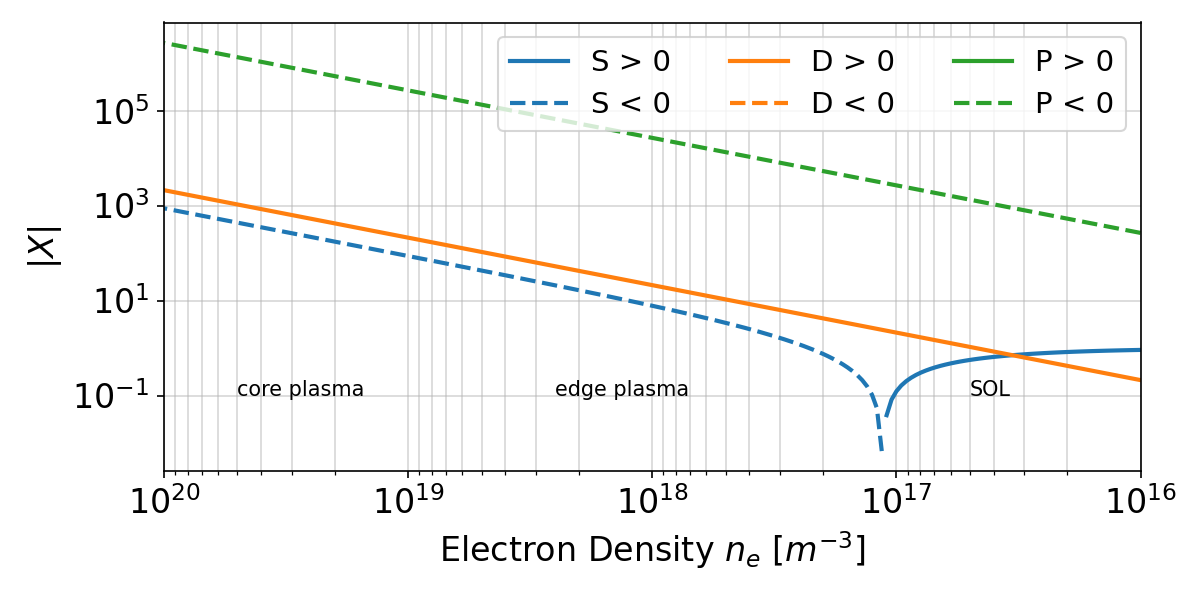
\includegraphics[width=1.0\linewidth]{figures/chap2/IC_SDP}
	\caption{Values of $S$, $D$ and $P$ terms in the Ion Cyclotron Range of Frequency.}
	\label{fig:icsdp}
\end{figure*}



% ###################################################
% ###################################################
\subsubsection{ICRF Dispersion Relation}
The roots of the dispersion equation Eqs.(\ref{eq:nperp_solution_general}) are approximatively in the ICRF\sidecite{Brambilla1998, usoltceva2019}:
\begin{subequations}
\begin{eqnarray}
n_{\perp, F}^2 &\approx& \frac{\left(R - n_\parallel^2 \right)\left(L - n_\parallel^2\right)}{S-n_\parallel^2} \\
			   &\approx& \left(S-n_\parallel^2 \right) - \frac{D^2}{S-n_\parallel^2} \nonumber \\
n_{\perp, S}^2 &\approx& \frac{P}{S}\left(S - n_\parallel^2 \right)
\label{eq:n_perp_square_approx_ICRF}		  
\end{eqnarray}
\end{subequations}
where the subscript $_F$ and $_S$ stands for \textit{Fast} and \textit{Slow} wave modes. The Figure~\ref{fig:nperpsquarevsne_ICRF} illustrates the typical range of $n_\perp^2$ values in tokamak plasma in the Ion Cyclotron Range of Frequency. 

\begin{figure*}[h]
	\centering
	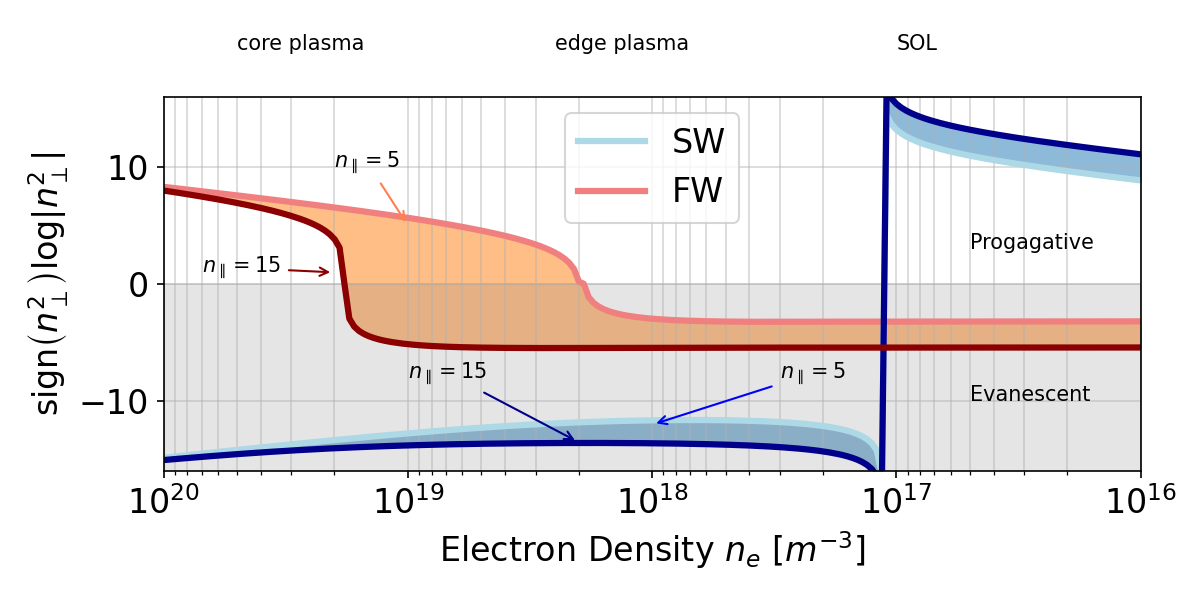
\includegraphics[width=1.0\linewidth]{figures/chap2/n_perp_square_vs_ne_ICRF}
	\caption{Perpendicular index $n_\perp^2$ from Eqs.(\ref{eq:nperp_solution_general}) (or Eqs.(\ref{eq:n_perp_square_approx_ICRF})) for Slow and fast waves for the typical range of electron density $n_e$ found in front of tokamak ICRF antenna ($f=50\,\si{MHz}$, $B_0=3\,\si{T}$). As antennas radiate a continuous spectrum of parallel indexes $n_\parallel$, low and high values are indicated.}
	\label{fig:nperpsquarevsne_ICRF}
\end{figure*}

\begin{marginfigure}
	\centering
	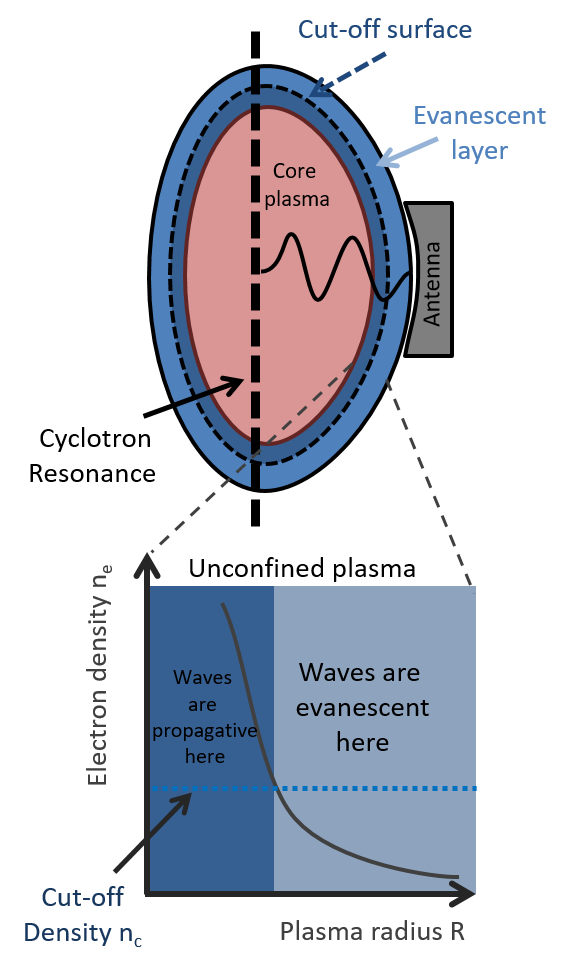
\includegraphics[width=1.0\linewidth]{figures/chap2/core_edge_antenna}
	\caption{Illustration of the different region in a tokamak. The core plasma is confined by following closed magnetic lines. The region defined by open field lines is the region where lie the antennas. The waves generated by the IC antennas are propagative only if the density is higher than a threshold, a cut-off density.}
	\label{fig:coreedgeantenna}
\end{marginfigure}
The Figure~\ref{fig:nperpsquarevsne_ICRF} shows that the Fast Wave mode, the one which is desired for heating the ions of the core plasma, becomes propagative for electron density beyond a \textit{cut-off} density $n_{c}$. This density depends of the RF frequency, the magnetic field and the parallel index excited by the antenna. Moreover, the high $n_\parallel$ component of the spectrum radiated by the antenna has to tunnel further away then the low $n\parallel$ part and tends to be filtered from the launched spectrum. In the ICRF for the Fast wave, the cut-off density $n_c$ is defined as: 
\begin{equation}
n_\parallel^2 = R
\end{equation}
which leads for a single ion plasma to: 
\begin{equation}
n_c \approx \Omega_i^2 \frac{\left(1 + \frac{\omega}{\Omega_i}\right)}{\frac{Z^2 e^2}{\varepsilon_{0} m_i}}n_\parallel^2 
\end{equation}

For effective tunnelling of the Fast wave launched by the antenna, located outside the unconfined region, the
plasma density in front of the antenna should be as high as possible, which highly depends on the distance between antennas and plasma. Hence this often requires the antenna to be close as possible to the confined plasma. However, this proximity has drawbacks: the heat fluxes from the plasma are impacting the antenna are higher and must be evacuated efficiently, leading to engineering issues.


% ###################################################
% ###################################################
\subsubsection{ICRF Wave Polarization}
Injecting the previous solutions into Eq.(\ref{eq:relation_disp_matr_froid}) leads to the polarization of these modes in the Stix frame:
\begin{subequations}
	\begin{eqnarray}
		\mbox{Fast wave: } & E_z = 0 & \frac{E_x}{E_y}=\frac{j D}{S - n_\parallel^2} \\
		\mbox{Slow wave: } & E_y = 0 & \frac{E_x}{E_z}=- \frac{n_\parallel n_{\perp,S} }{S - n_\parallel^2}
	\end{eqnarray}
\end{subequations}

The key engineering issue in designing a ICRH antenna is to effectively radiate fast waves and not slow waves, as slow waves may create undesirable effects on the plasma known as \textit{RF sheaths}\sidenote{RF sheaths are briefly discussed in Section~\ref{sec:RF_sheaths}).}.

% ###################################################
% ###################################################
\subsubsection{ICRF Antennas Main Figures of Merit}
The effectiveness of Fast wave coupling is in practice measured by the maximum radiated power $P_{\mathrm{rad,max}}$ by an antenna to a given plasma and can be defined in various ways. Assuming the antenna is modelled by a lossless transmission line of characteristic impedance $Z_0$ loaded with a  resistance $R_c$, the maximum power delivered to the load would be:
\begin{equation}
P_\mathrm{rad,max} = \frac{1}{2} R_c I^2_{\mathrm{max}} = \frac{R_c}{2 Z_0^2} V_\mathrm{max}^2
\end{equation}
where $I_\mathrm{max}$ and $V_\mathrm{max}$ are the maximum peak RF current and voltage at the load. The amplitude of the maximum current on the transmission line $I_\mathrm{max}$ depends on the geometry of antenna system and of the plasma parameters. Hence, $R_c$ can be seen as a measure of the system coupling efficiency and is called the \textit{coupling} or \textit{loading} resistance. In reality however, the RF current or voltage along the strap are not constant, hence the coupling resistance can be defined using the integral over the arc length $s$ along the strap:
\begin{equation}
	R_c = \frac{2 P_{\mathrm{rad}}}{\int_s |I(s)|^2 \diff s}
\end{equation}
where $P_\mathrm{rad}$ is the time-averaged radiated power. In numerical simulation, this power can be obtained from the Poynting theorem in the $\kbf$-space as:
\begin{equation}
	P_\mathrm{rad}
	=
	\Re
	\left\{ 
	\frac{k_{0}^{2}}{4\pi^{2}}
	\iint
	\left[
	\Ebf \left(n_{y},n_{\parallel}\right)
	\times
	\Hbf^{*} \left(n_{y},n_{\parallel}\right)
	\cdot\hat{\xbf}
	\right]
	\right\} 
	\diff n_y 
	\diff n_\parallel
\end{equation}
During experiment, it can be obtained from power, voltage or current measurements, and its definition also vary from machine to machine. ICRF coupling theory is discussed in details \sidecite{messiaen1982} and compared with experiments in \sidecite{koch1988}.


The scaling of $R_c$ for an increasing electron density with a gradient length $d_c$ from the antenna to the cut-off density $n_c$,  is given by:
\begin{equation}
	R_c \propto \exp\left(- \nu \left< k_\parallel \right> d_c \right)
\end{equation}
where $\nu$ is a constant constant representing the plasma density and its gradient and $\left< k_\parallel \right>$ a characteristic factor depending on an integration over the radiated spectrum by the antenna.  On Tore Supra, this scaling has been shown to be\sidecite{clairet2004}:
\begin{equation}
R_c \propto exp\left(- 2 \left< k_\parallel \right> d_{\mathrm{sco}} \right)
\end{equation}
where $d_{\mathrm{sco}}$ is the distance from the antenna straps to the density cut-off location. 
%KSTAR \sidecite{bae2003-1, wang2010}







% ###################################################
% ###################################################
% ###################################################
\subsection{Lower Hybrid Range of Frequencies}\label{sec:lhcd}
In the Lower Hybrid Range of Frequencies, i.e. for $\Omega_i \ll \omega \ll \Omega_e$, the $S$, $D$ and $P$ parameters can be simplified at the lead order \cite[p.222]{Brambilla1998} to (Figure~\ref{fig:lhsdp})):
\begin{subequations}
	\begin{eqnarray}
		S &\approx& 1 - \frac{\omega_i^2}{\omega^2} + \frac{\omega_e^2}{\Omega_e^2} \approx 1 \\
		D &\approx& - \frac{\omega_e^2}{\omega \Omega_e} \approx 0 \\
		P &\approx& 1 - \frac{\omega_e^2}{\omega^2} = 1 - \frac{n_e}{n_c}
	\end{eqnarray}
\end{subequations}
where $n_c$ is the cut-off density for the Slow-wave defined for $P=0$ or:
\begin{equation}
	n_c = \frac{m_e \varepsilon_{0}}{e^2} \omega^2 \approx  0.0124 f^2
	\label{eq:lh_cutoff_density}
\end{equation}
\begin{figure*}[h]
	\centering
	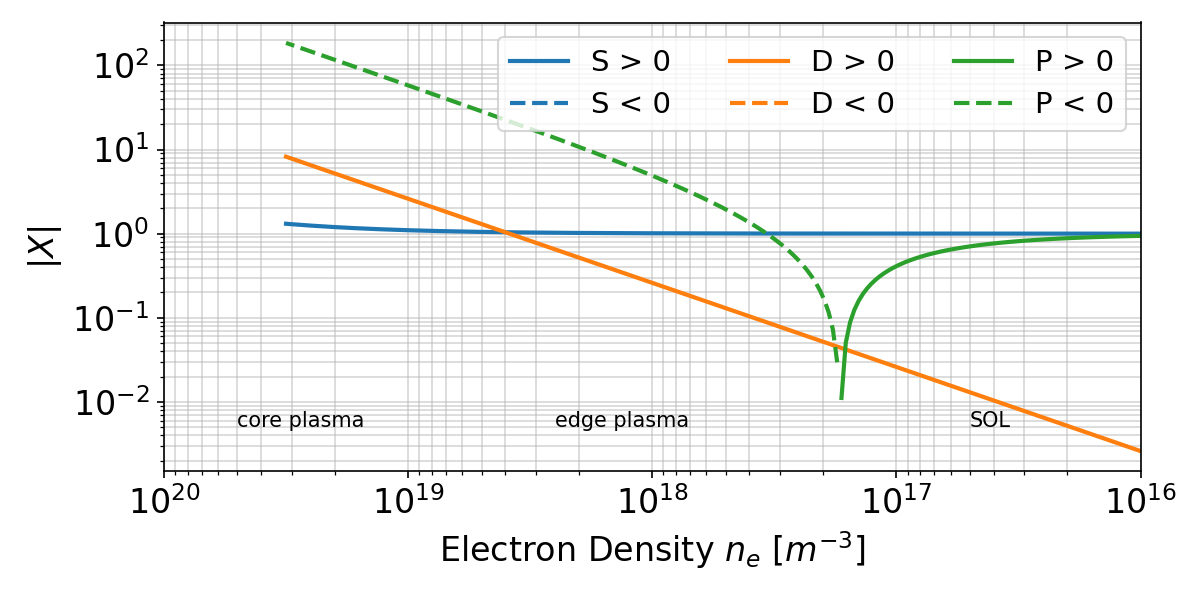
\includegraphics[width=1.0\linewidth]{figures/chap2/LH_SDP}
	\caption{Values of $S$, $D$ and $P$ terms in the Lower Hybrid Range of Frequency. ($f=3.7\,\si{GHz}$,$B_0=3\,\si{T}$).}
	\label{fig:lhsdp}
\end{figure*}


% ###################################################
% ###################################################
\subsubsection{LHRF Dispersion Relation}
In the LHRF, the solution of the dispersion relation reads:
\begin{subequations}
	\begin{eqnarray}
		n_{\perp,F}^2 &\approx& S - n_\parallel^2  \approx 1 - n_\parallel^2 \\
		\label{eq:n_perp_square_FW_LHRF}
		n_{\perp,S}^2 &\approx& \frac{P}{S} \left(S - n_\parallel^2\right) \approx P(1- n_\parallel^2)
		\label{eq:n_perp_square_SW_LHRF}
	\end{eqnarray}
	\label{eq:n_perp_square_LHRF}
\end{subequations}

\begin{figure*}[h]
	\centering
	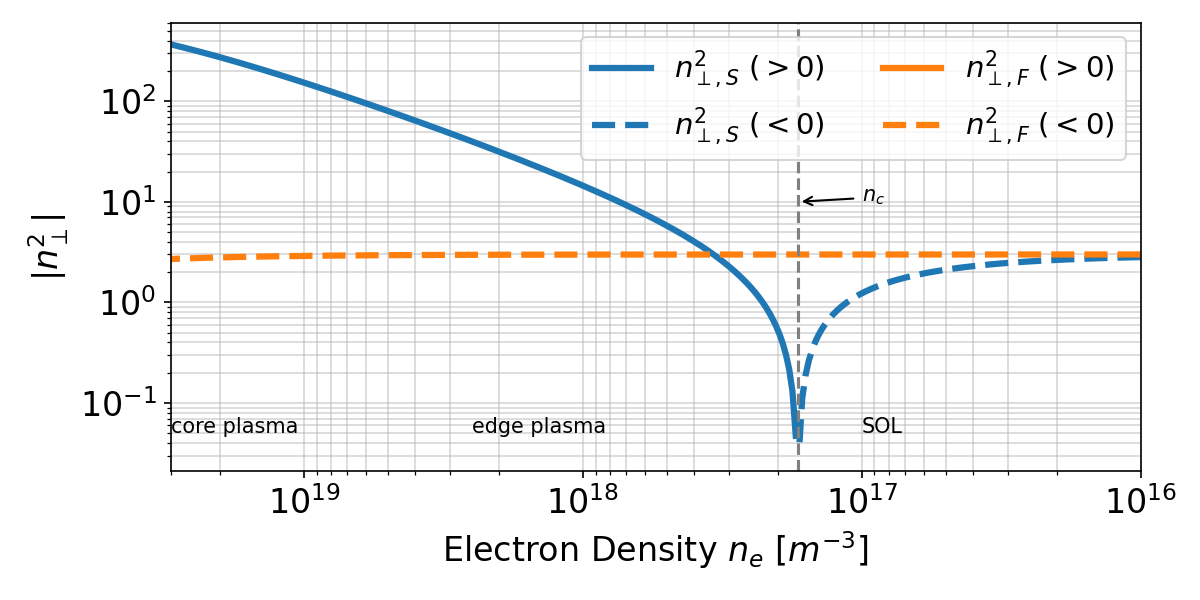
\includegraphics[width=1.0\linewidth]{figures/chap2/n_perp_square_vs_ne_LHRF}
	\caption{Perpendicular index $n_\perp^2$ from Eqs.(\ref{eq:nperp_solution_general})   for the typical range of electron density $n_e$ found in front of tokamak LHRF antenna ($f=3.7\,\si{GHz}$, $B_0=3\,\si{T}$).}
	\label{fig:nperpsquarevsne_LHRF}
\end{figure*}

% ###################################################
% ###################################################
%\subsubsection{Resonance Cone}
%Bellan and Porkolab PRL 34, 124, 1975.

% ###################################################
% ###################################################
\subsubsection{LHRF Wave Polarization}
Similarly, the electric field polarisation in the LHRF gets:
\begin{subequations}
	\begin{eqnarray}
	\mbox{Fast wave: } & E_z = 0 & \frac{E_x}{E_y}= \frac{j D}{S - n_\parallel^2} \\
	\mbox{Slow wave: } & E_y = 0 & \frac{E_x}{E_z}=- \frac{n_\parallel n_{\perp,S} }{S - n_\parallel^2}
	\end{eqnarray}
\end{subequations}

% ###################################################
% ###################################################
\subsubsection{Wave propagation conditions}
In order for the RF power to reach the plasma core, the excited waves by a LHCD launcher must satisfy different criteria: 

\begin{itemize}
	\item  A \emph{cut-off condition}: the electron density in front of the launcher must be close or higher than the slow-wave electron \emph{cut-off density}, given by Eq.(\ref{eq:lh_cutoff_density}), which increases as the square of the source frequency. 
	\item A propagation condition: in order for the Slow and fast waves in the LHRF to propagate into the magnetized plasma, from Eqs.(\ref{eq:n_perp_square_LHRF}) excited waves must have an absolute value of the parallel index greater than one, i.e. $|n_{\parallel}|>1$ 
	\item An accessibility condition: in order for the slow waves accessing the plasma core to not be mode-converted into fast waves, a minimum value of $n_{\parallel}$ for a given plasma density and magnetic field is requested\sidecite{golant1972}:
	\begin{equation}
	|n_{\parallel} |>| n_{\parallel \mathrm{access}} | 
	\approx 
	\sqrt{1 
		- \frac{\omega_{pi}^2}{\omega^2} 
		+ \frac{\omega_{pe}^2}{\omega_{ce}^2}}
	+ \frac{\omega_{pe} }{| \omega_{ce} |}
	\label{eq:accessibilit_condition_LH}
	\end{equation}
\end{itemize}

When the accessibility condition is satisfied, the slow and the fast branch of the dispersion relation are separated and the LH waves can reach the core plasma. Inversely, for a given $n_{\parallel}$, the previous condition leads to an upper limit for the density (inside the plasma), above which the wave can’t propagate.

% ###################################################
% ###################################################
\subsubsection{LHRF Antennas Main Figures of Merit}
There are three important figures of merit to measure the efficiency and
performance of a LH launcher. The first one is the $\mathbf{k}$-space radiated power spectrum density $\diff p(n_y, n_\parallel)$, defined as the $k$-space Poynting vector\marginnote{Integrating the power spectrum density over the entire $n$-space gives the transmitted power to the plasma.}:
\begin{equation} 
\diff p
\left(n_{y},n_{\parallel}\right)
=\Re\left\{ \frac{k_{0}^{2}}{4\pi^{2}}
\left[\tilde{\mathbf{E}}
\left(n_{y},n_{\parallel}\right)
\times
\mathbf{\tilde{H}^{*}}\left(n_{y},n_{\parallel}\right)
\cdot\hat{\xbf}
\right]
\right\} 
\end{equation}
Since it is often assumed that the plasma is infinite in the $y$ direction (slab model), the main acceptation of the power spectrum density is $\diff p(n_\parallel)$, which corresponds to integrate the contribution of all the $n_{y}$ for a given $n_{\parallel}$:
\begin{equation}
\diff p\left(n_{\parallel}\right)=\int_{-\infty}^{+\infty}\! \diff p\left(n_{y},n_{\parallel}\right)\, \diff n_y
\end{equation}
This quantity represents the amount of power excited by the launcher for each parallel index $n_\parallel$. The relation between this power spectrum and the array excitation is related to the Fourier transform of the electromagnetic field at the plasma-antenna interface.

The second one is the ratio of the reflected power (at the mouth or at the end of the launcher) to the input power, named the reflection coefficient $R_C$\sidenote{Which should not be confounded with the coupling resistance defined for ICRF.} and often expressed in percent:
\begin{equation}
	R_C = P_r/P_i
\end{equation} 

The third one is the directivity of the launcher, which is the fraction of the power spectrum over its total power content. It can be viewed as the fraction of the power that goes toward one toroidal direction over the total coupled power. One can define the directivity as:
\begin{equation}
D = \frac{\int_{n_\parallel > 0}  \diff p(n_\parallel) \diff n_\parallel}{\int \diff p(n_\parallel) \diff n_\parallel} 
\end{equation}

Since the wave field at the launcher aperture (and thus the launcher spectrum) depends on both the antenna and the plasma, numerical coupling codes are required to make a self-consistent numerical evaluation of the coupling. Different types of launchers have been developped to balance the sometimes conflicting requirements of experimental flexibility, reduced complexity and thermal constraints. These antennas are discussed in Section~\ref{sec:LHCD_antennas_general}.


%The RF power is coupled by the launcher to the plasma, which means that the electromagnetic waves in the launcher’s waveguides are converted to (mainly) slow waves in the plasma. In the LH range of frequencies (~2 to 8 GHz), the wavelength of the RF waves in the plasma is well below the typical beam size, which itself is smaller than the equilibrium non-uniformity scale. It this situation, the evolution of the waves in the plasma can be described by the \emph{ray-tracing} formalism. Since the evolution of the electron population can be described with Fokker-Planck calculation, the combination of the both tools is standard for modelling LHCD experiments\sidecite{bonoli1982, peysson2012}.
%
%As said before, the LHCD launcher is a phased array of waveguide which excites a slow plasma wave. The following calculations taken from current drive theory illustrate the basic requirements of the LHCD launcher in order to optimize the current drive efficiency. 
%
%In the plasma, the incremental current $\Delta j$ carried by an electron of electrical charge $q=-e$ and accelerated from a parallel velocity $v_\parallel$ to $v_\parallel + \Delta v_\parallel$ is:
%$$\Delta j = q \Delta v_{\parallel}$$
%
%The incremental increase of kinetic energy is:
%$$\Delta E = m v_{\parallel} \Delta v_{\parallel}$$
%
%Eliminating $\Delta v_{\parallel}$ leads to an incremental current: 
%$$\Delta j = \Delta E \; q/(m v_{\parallel})$$ 
%
%Let $\nu_\mathrm{coll}$ be the Coulomb collisional frequency. At first order \footnote{Rigourously, the mathematical tool for a complete description of multiple scattering processes in the velocity-space is the Boltzman equation. The collision term modelling the multiple particles Coulomb collisions in this equation can be modelled by a collision term of the Fokker-Planck type.} the incremental energy input $\Delta E$ persists for a time $1/\nu_\mathrm{coll}$. The associated (steady-state) RF input power $\Delta P$ required is thus: 
%$$\Delta P = \nu_\mathrm{coll} \Delta E$$ 
%
%From the two previous equations, the ratio of the incremental current to the RF input power is:
%$$\Delta j/ \Delta P = q / (m \nu_\mathrm{coll} v_{\parallel})$$
%
%This suggests that more current can be driven with low parallel velocity electrons. However, fast electrons collide less often than slower, as the Coulomb collision cross section falls off with increasing relative velocity as $\nu_\mathrm{coll} \propto n_e/v_{\parallel}^3$ (for parallel velocity larger than the thermal velocity). It follows that the previous ratio is proportional to: 
%
%$$\Delta j/ \Delta P \propto (v_{\parallel}^2 q) / (m n_e)$$
%
%this means that high current drive efficiency can be reached from fast electrons. Thus, it is actually more effective to push fast electrons than slower. Even if it may be energetically more expensive to accelerate fast electrons, this energy deposition need occurs less often because current last longer when carried by relatively less collisional electrons \sidecite{fisch1987}. 
%
%For the purpose of current drive with LH waves, the Landau damping is the dominant absorption mechanism. Landau damping is a collision-less damping process in which particles exchange energy with waves travelling with the nearly same phase velocity parallel to the magnetic field, that is, for particle parallel velocity $v_{\parallel}$ satisfying resonant condition:
%
%$$\omega – k_{\parallel} v_{\parallel} = 0 $$ 
%
%where $k_{\parallel}=k_0 n_{\parallel}$ is the parallel wavenumber of the wave, $n_{\parallel}$ the parallel index of refraction and $k_0= \omega/c$ the wavenumber in vacuum. From the previous relation one deduces that the LHCD launcher must excite waves satisfying the resonant condition $v_{\parallel}=c/n_{\parallel}$. As for the slow wave to be able to penetrate into the plasma the parallel index must be greater than one and also greater to $|n_{\parallel \mathrm{access}}|$, typical LHCD launchers in current tokamaks excite a main parallel index between $n_{\parallel 0}$=1.5 to 3.0. 
%
%However, in many past and present LHCD experiments, the resonant velocity $v_{\parallel 0}=c/n_{\parallel 0}$ corresponds to supra thermal region where the number of electrons should be in principle too small for any significant wave damping to take place and to account for the observed current drive. Indeed, strong wave damping on a Maxwellian distribution with temperature $T$ requires the wave damping to be no larger than four times the thermal velocity $v_T=\sqrt{k T/m}$. This paradox is commonly referred to as the \emph{spectral gap} problem and is an active area of research. Various explanations are proposed to explain this spectral gap, among these the toroidal effects on the wave propagation that can cause sufficient up-shift (increase of the parallel wavenumber) in the parallel refraction index $n_{\parallel}$ to “fill” the spectral gap, non-linear interactions such as \textit{parametric decay instabilities} (PDI), diffraction effects or power density spectrum fluctuations. 



\clearpage
% ###################################################
% ###################################################
\section{The ALOHA code}\label{sec:ALOHA}
\marginnote{Parts of this section are taken from paper \citeauthyear{hillairet2010}.}
% ###################################################
\subsection{Context of this work}
The theory of the coupling between LHRF antennas and the plasma has been developed in \sidecite[-0.5cm]{brambilla1976-1,brambilla1979} for 2D waveguides (parallel plates infinite the poloidal direction) and refined after for rectangular waveguides in \sidecite{bers1983}. In 2007, best known linear coupling codes used to design present operating antennas are Slow Wave ANtenna (SWAN) \sidecite{litaudon1990, moreau1984} or GRILL3D \sidecite[+1cm]{irzak1995}. In these codes, the toroidal lines of waveguides are assumed to be infinite in the poloidal direction and are described using a modal expansion. The modal description of the field makes possible to simulate large antennas with a moderate computing cost but the code cannot handle realistic geometry.

In order to improve the antenna-plasma coupling description of SWAN code while keeping its low computational cost, a code named Advanced LOwer Hybrid Antenna (ALOHA) has been developed\sidenote{The code has been initially written by S.Berio and Ph.Bibet in 1994 \cite{berio1996}, then improved later by Damien Voyer in 2006. Since 2008, I continued to develop the code, completely rewritten since in modern Fortran with a Matlab front-end. The code development was first versioned on CEA internal servers since Nov.2009 before being \href{https://github.com/jhillairet/ALOHA}{open-sourced in on github} since Sept.2015. ALOHA has been used by different user in fusion laboratory worldwide: MIT/PSFC, ASIPP, NFRI, IPR, IPP/Prague, etc. Since 2008, ALOHA has been cited in more than 130 references.}. In ALOHA, LH antennas may be modelled by any RF full-wave commercial software or home-made code\footnote{For optimization process, a plug-in named HAMAC (Hybrid Antenna Modelling for the ALOHA Code) has been developed in the frame of the master training of Melanie Preynas in 2009 and Michal Kazda in 2010.}. The plasma coupling is calculated from a fast classical 1D modelling that describes the effect of the slow wave only\cite{brambilla1976-1} or from a more advanced 2D modelling that implies the contribution of both fast and slow waves\cite{brambilla1979, bers1983, irzak1995}.
These calculations are based on the linear cold plasma theory and non-linear effects, such as thermal effects ("warm" dielectric tensor) and ponderomotive force have not been taken into account in the present analysis. However, some specific developments have been brought in one hand, to describe a more realistic electron density profiles taking into account the close environment of LH antennas and in the other hand, to avoid computational difficulties when the antenna is large. These assumptions let ALOHA to solve a case in a couple of seconds up to 2 hours on a 2008 desktop computer, depending on the number of waveguides of the antenna and the plasma model chosen. By comparison, a boundary element code such as the Torino Politecnico Lower Hybrid Antenna (TOPLHA) code\sidecite{milanesio2011}, required at that time high-end or super-computers to be solved. At the same time, finite element software such as COMSOL just began to be able to treat materials with generic temporally-dispersive dielectric tensors. Such approach leaves absolute freedom in the description of the antenna geometry and of the plasma within the collisional cold plasma approximation but required high computation time or resources \sidecite{meneghini2009-1, shiraiwa2011-1}. Nowadays, the Finite-Element Method can be used in more daily basis for LHCD coupling as discussed in Section~\ref{sec:LHCD_FW_antena_coupling}. However, it is still inconsistent with intensive use, for example in daily experiments when one has to evaluate the effect of modules tripping on the radiated spectrum or during antenna design stage, where many calculations may be expected. In order to interpret and improve present day experiments and to design future antennas, an advanced but fast and convenient modelling tools is still convenient.

The next section recall the key elements of the linear coupling theory. ALOHA specificities are detailed, such as the use of generalized scattering matrix use, the 2D grill modelling and the two electron density gradients profile. The Section~\ref{sec:ALOHA_TS} is devoted to experimental comparisons and simulation benchmarks on Tore Supra antennas. 


\subsection{Main assumptions}\label{sec:Theory}

\subsubsection{Network description}\label{sec:network_description}

The LHCD antenna of past or present experiments (JET, Alcator C-Mod, FTU, EAST, KSTAR, Tore Supra/WEST, etc.) are designed to launch an asymmetric parallel wavenumber spectrum where most of the power is generated at a low parallel refractive index $\left|n_{\parallel}\right|\approx2$. This is usually achieved by phasing the forward waves in waveguides which are stacked along the static magnetic field. This phasing can be obtained externally in the transmission line feeding of the antenna \sidecite[-2cm]{bernabei2003, bae2003, park2010} or directly inside the antenna when E-plane power dividers -- usually called "multijunction" \sidecite{moreau1984} -- are associated with built-in phase shifters \sidecite[+0.5cm]{ekedahl2009-1, bo-jiang2006, zhao2010}.

Here, the term "module" refers to the unit of the antenna composed of one "input" waveguide fed by the power source and one or several "output" waveguides facing the plasma, and the "grill" refers to the plane containing all the open ended waveguides of the antenna. A complete LH antenna can be made of many different modules, stacked in the toroidal or poloidal directions. A simple example is depicted in Figure~\ref{fig:geometry_antenna}.

In the ALOHA code, the plasma coupling of a LH grill antenna is split in two parts: the modeling of the modules and the modeling of the grill in front of the plasma. 

Firstly, the electromagnetic characterization of a module is obtained using some RF software or code, which results in the calculation of the scattering matrix of a module $\mathbb{S}_{\mbox{module}}$ in which only the propagating modes are taken into account. This matrix quantifies the coupling between all inputs and outputs of the RF structure \cite{kurokawa1965}. 

Secondly, the coupling to the plasma of all the output waveguides that compose the grill is considered. At this stage, evanescent modes excited at the end of the waveguides are also taken in account. Thus, the grill is characterized by a $N$-port network where $N=N_{\mbox{wg}}\times N_{\mbox{modes}}$ is the number of ports, $N_{\mbox{wg}}$ the total number of output waveguides and $N_{\mbox{modes}}$ the number of electromagnetic modes in each waveguide. A scattering matrix $\mathbb{S}_{\mbox{grill/plasma}}$ of dimensions $N\times N$ is then derived using the approach detailed in Section~\ref{sec:grill_modeling}: this matrix quantifies the coupling between the different ports. In such a modeling, each mode is associated to a port \cite{Harrington2001}; a port can coincide either with the principal mode that propagate inside an output waveguide or with a higher order mode excited at the end of an output waveguide. 

Finally, following the well known network approach, both modeling are combined: the ports in the scattering matrices $\mathbb{S}_{\mbox{module}}$ and $\mathbb{S}_{\mbox{grill/plasma}}$ that correspond to the same mode in a waveguide are identified and the global response of the antenna can then be extracted and directly compared to experimental data.

For a better understanding, let us consider the example of the antenna shown in Figure~\ref{fig:geometry_antenna}. It is composed of one toroidal line of waveguides shared into two modules. Each module is a multijunction in which a large input feeding waveguide is split into four smaller output waveguides; the output waveguides are said to be active waveguides since they are connected to the input waveguide inside the module. The modules are separated by a short circuited waveguide; this waveguide is isolated and consequently is said to be passive. Moreover, there is also one passive waveguide on each side of the antenna. Each module is characterized by a scattering matrix $\mathbb{S}_{\mbox{module1}}$ and $\mathbb{S}_{\mbox{module2}}$.

%
\begin{figure}[h]
	\centering{}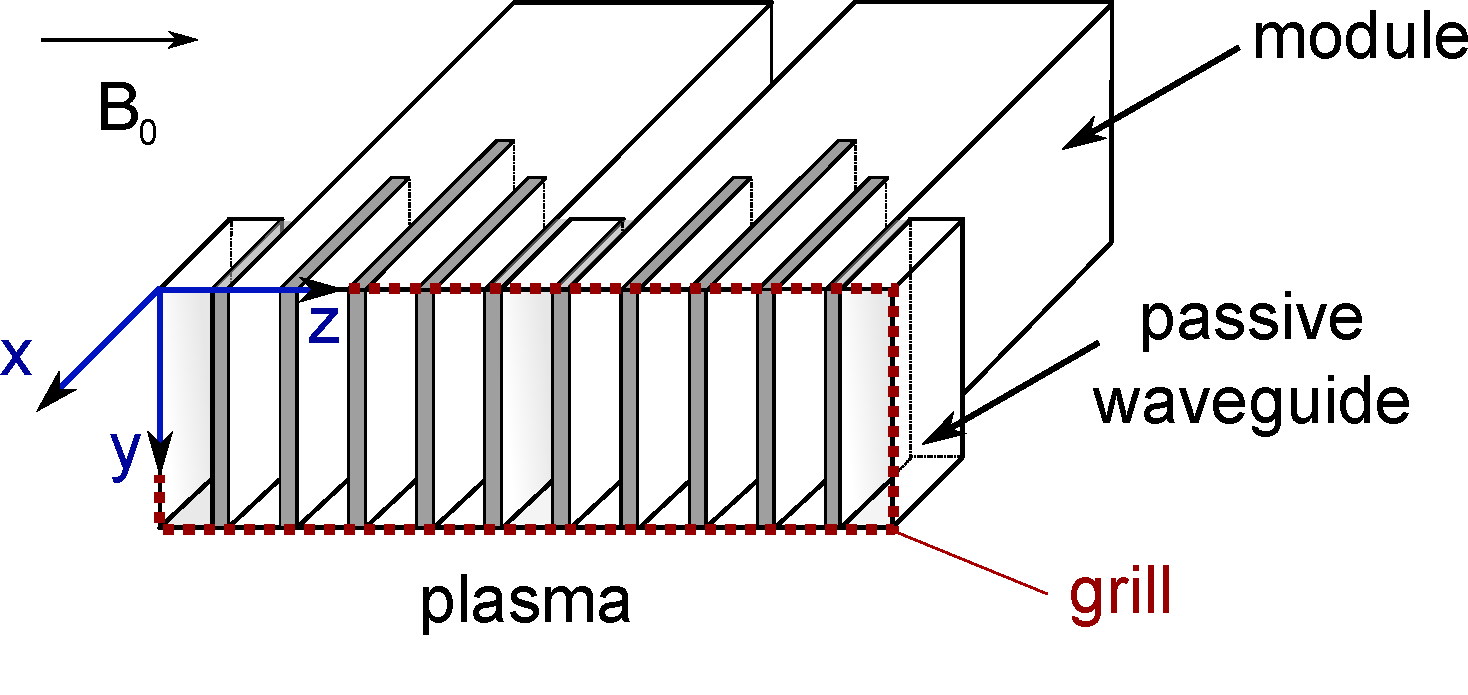
\includegraphics[width=0.9\textwidth]{figures/chap2/ALOHA/figure1} 
	\caption{A typical LH (multijunction) antenna structure. In this example, the
		antenna is made of two multijunction modules stacked in the toroidal
		($z$) direction. One passive waveguide is inserted between both modules
		and on each side of the antenna.\label{fig:geometry_antenna} }
	
\end{figure}


Suppose that, in front of the plasma, two modes are excited inside the output waveguides: the principal mode $\TE_{10}$ and the evanescent mode $\TM_{11}$. The network modeling of this problem is given in figure \ref{fig:network_representation}. In that representation, a port in a N-port network is described by a terminal. Thus, each of both modules is characterized by a 5-port network (1\,input waveguide $\times$ 1\,mode + 4\,active waveguides $\times$ 1\,mode) and the coupling of the grill with the plasma is modeled by a 22-port network (\textit{\emph{8\,active waveguides $\times$ 2\,modes + 		3\,passive waveguides $\times$ 2\,modes}}). The terminals in the 22-port network that coincide with the principal mode of the active waveguides in the modules are connected to the corresponding terminals in the 5-port network. The terminals in the 22-port network that coincide with the principal mode of the passive waveguides are shunt on a piece of transmission line ended by a short-circuit to model the reflection of the wave. The terminals in the 22-port network that coincide with the evanescent modes are shunt on the imaginary mode impedance of the output waveguide, which is equivalent to consider that those modes carry reactive energy in a waveguide of infinite length. Finally, the antenna reduces to a 2-port network in which the ports correspond to the input feeding waveguide of both modules and the global scattering matrix of the antenna is a $2\times2$ matrix $\left(\mathbb{S}_{\mbox{access}}\right)$. This formalism allows the code to fully take into account the coupling of the modes in the waveguides.

%
\begin{figure}[h]
	\centering{}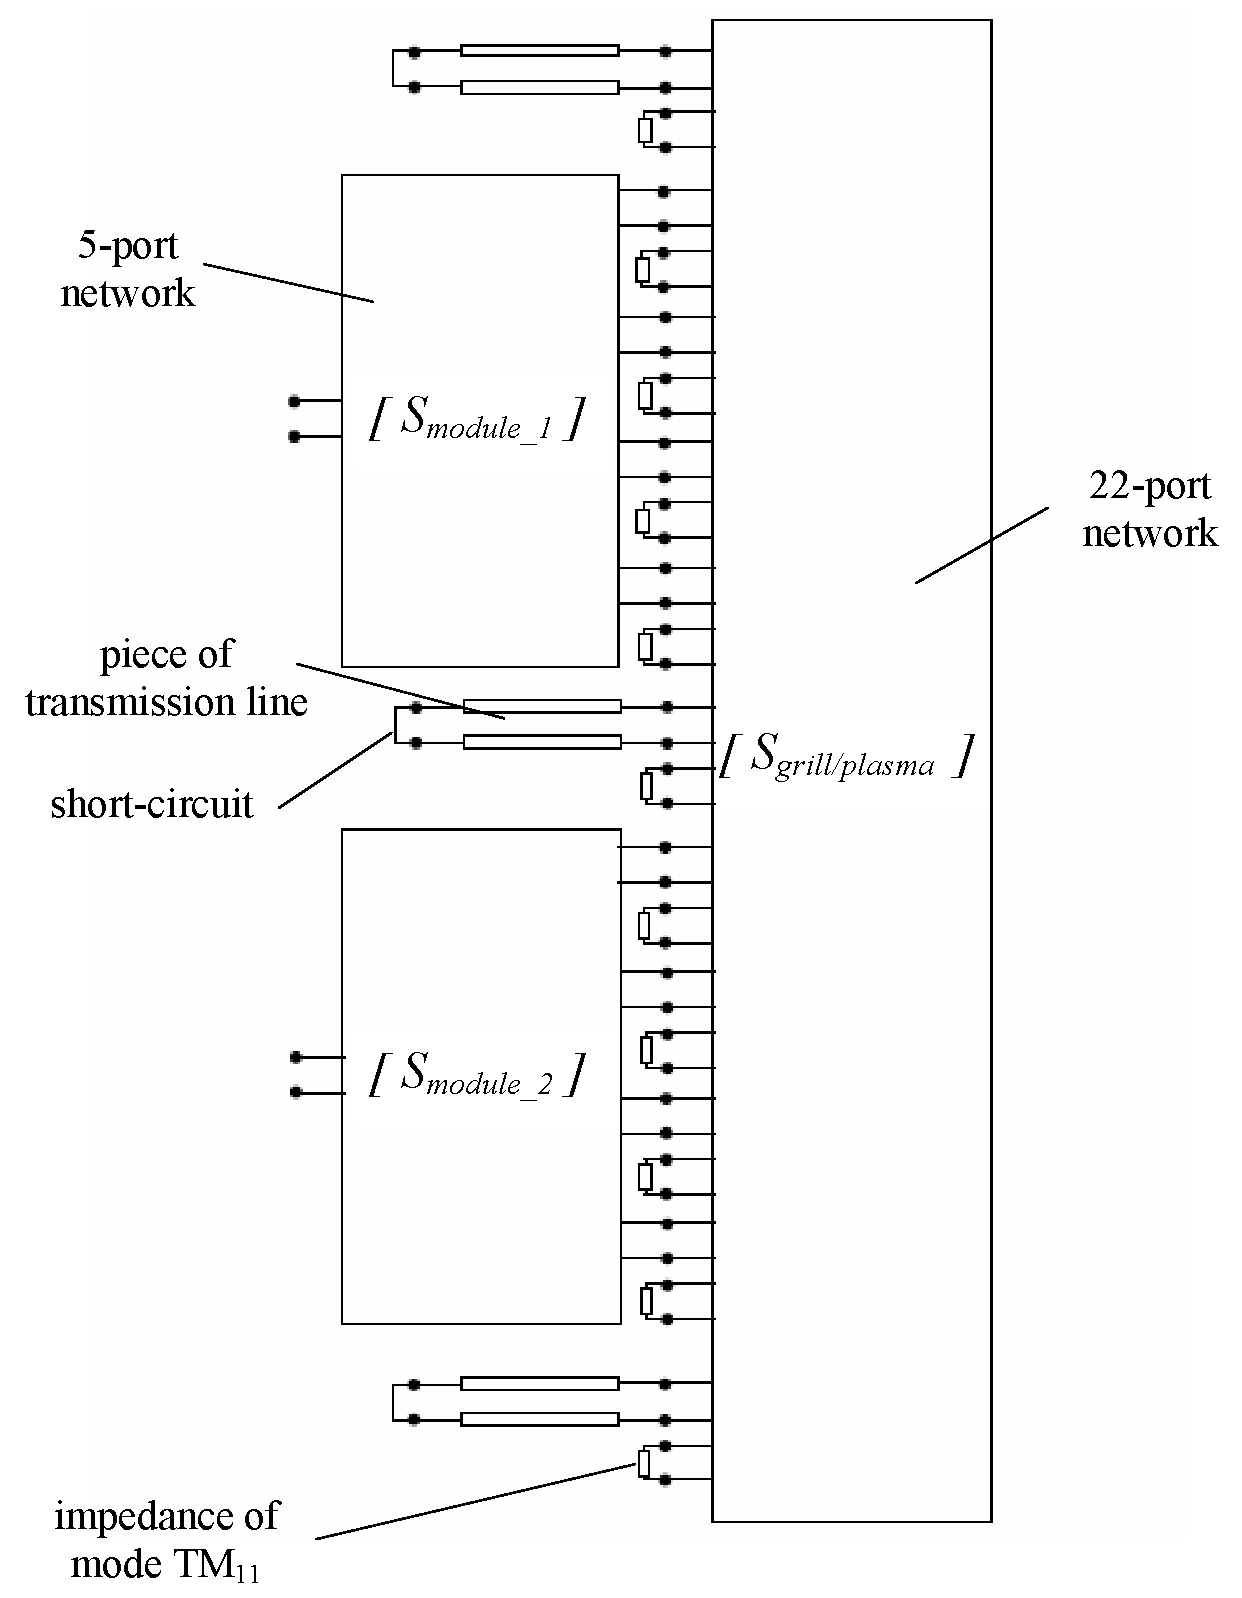
\includegraphics[width=0.7\textwidth]{figures/chap2/ALOHA/figure2} \caption{Illustration of the modeling of the antenna described in figure \ref{fig:geometry_antenna}
		using the N-port concept.\label{fig:network_representation} }
	
\end{figure}



\subsubsection{Module modelling}\label{sub:module_modeling}

Lower Hybrid experiments show that the coupling efficiency not only depends on the plasma configuration but also on the antenna structure. Antennas are often designed in order to minimize the reflected power from the plasma to the RF sources, thus limiting the need of complex and expensive klystron protection systems. Multijunction concept is frequently used in tokamaks in order to create large waveguide arrays. The necessary phase shifts between adjacent waveguides used to launch non-symmetrical parallel wavenumber spectrum is usually obtained in the design by adjusting the relative guide heights \sidecite{litaudon1992}. These built-in phase shifters create multiple passages of the waves through the structure, which lead to a reduction of the reflected power to the RF sources as well as an increase of the electric field strength or an increase of secondary peaks in the radiated power spectrum. Thus, the RF design of such antennas is less straight-forward than simple open-ended waveguides and an accurate RF characterization is required to analyze the experimental data.

The coupling efficiency requires the measurement of the forward and reflected electric fields in all waveguides which in principle can be done but requires the installation under vacuum of a very large number of probes\sidecite{jacquet1997, meneghini2010}. For an easier maintenance of the RF system, the use of a single bi-directional coupler at the module input in the pressurized transmission line is usually preferred. With this scheme, the electric field map at the plasma-antenna interface, needed to compute the launched parallel index $n_{\parallel}$, is only accessible by computation. In order to directly compare theoretical coupling predictions to experimental RF measurements, the RF description of each module have to be considered incorporating all the RF components in line from the plasma up to the RF probes location. Thus, the realistic wave propagation inside each module, through multijunctions and power splitters (such as hybrid junctions, magic tees or mode converters) has to be taken into account. 

Commercial RF softwares, for example ANSYS HFSS, CST Studio or COMSOL, are convenient tools to design and optimize such components. In ALOHA, the scattering matrix calculated by these codes that describe the modules of the antenna can be directly used as input. Once the antenna's module scattering matrices calculated ($\mathbb{S}_{\mbox{module}}$), they are used as input for ALOHA to simulate the coupling between the modules and the plasma, as explained in the next sections.


\subsubsection{Grill-plasma modelling}\label{sec:grill_modeling}

\paragraph{Plasma description}\label{sec:dielectric_tensor}

Lets consider the geometry shown in Figure~\ref{fig:geometry_antenna}. The static magnetic field $\mathbf{B}_{0}$ is assumed to be in the $z$ direction and vary as well as the plasma density in $x$ direction. This hypothesis is specifically valid for large tokamak such as ITER or tokamak with high aspect ratio in which the angle between the magnetic field and the narrow waveguide is small. The interface between waveguides and plasma is set at $x=0$. The plasma is considered homogeneous
in $y$ and $z$ directions. The electromagnetic field scattered by the antenna is supposed to be dissipated far away from the coupling region so that the coupling problem is treated as a problem of radiation in a semi-infinite medium independently of the absorption in the core plasma. In such a modelling, the propagation into the plasma core is not calculated, meaning that effects such as mode conversion are not taken into account. 

From Maxwell's equations, we recall that the electromagnetic field in a cold plasma in the absence of source satisfies the vector wave equation Eq.(\ref{eq:wave_equation}):
\begin{equation}
\left(\nabla\times\nabla\times-k_{0}^{2}\mathbb{K}\cdot\right)\left|\begin{array}{c}
\mathbf{E}(\mathbf{r})\\
\mathbf{H}(\mathbf{r})\end{array}\right.=0
\end{equation}

where $\mathbf{E}$ and $\mathbf{H}$ are the electric and magnetic fields, $\mathbf{r}=x\mbox{\ensuremath{\hat{\mathbf{x}}}}+y\hat{\mathbf{y}}+z\hat{\mathbf{z}}$ is the space vector coordinates and $k_{0}=\frac{\omega}{c}$ the free-space wavenumber. In the vicinity of the grill, the plasma is described by its (normalized) cold dielectric tensor $\mathbb{K}$ Eq.(\ref{eq:stix_K}) which is recalled here: 
\begin{equation}
	\mathbb{K}(x,\omega)=\left[\begin{array}{ccc}
	S & jD & 0\\
	-jD & S & 0\\
	0 & 0 & P\end{array}\right]
	\label{eq:dielectric_tensor}
\end{equation}
where parameters $S$, $D$ and $P$ are defined by Eq.(\ref{eq:stix_SDP}) and depend on radial position $x$ and wave frequency.

%\begin{eqnarray}
%S(x,\omega) & = & 1-\sum_{s}\frac{\omega_{p,s}^{2}}{\omega^{2}-\Omega_{c,s}^{2}}\label{eq:stix_sum}\\
%D(x,\omega) & = & \sum_{s}\frac{\Omega_{ci}}{\omega}\frac{\omega_{p,s}^{2}}{\omega^{2}-\Omega_{c,s}^{2}}\label{eq:stix_difference}\\
%P(x,\omega) & = & 1-\sum_{s}\frac{\omega_{p,s}^{2}}{\omega^{2}}\label{eq:stix_plasma}
%\end{eqnarray}
%where $\omega$, $\Omega_{c,s}$ and $\omega_{p,s}$ are respectively the RF source, the cyclotron and the plasma angular frequencies of the species $s$.

% ####################################################################
\paragraph{Grill description}
The transverse (perpendicular to the $x$ direction) electromagnetic field $\mathbf{E}_{t,\mbox{grill}}$, $\mathbf{H}_{t,\mbox{grill}}$ at the end of the output waveguides, i.e. in the $x=0$ grill plane, can be expanded as a series of excited modes in similar way than Eq.(\ref{eq:voltage_current_lossy_line}) from Chap.\ref{chap:RF_fundamentals}:
\begin{eqnarray}
\mathbf{E}_{t,\mbox{grill}}(x=0,y,z) & = & \sum_{n=1}^{N}\sqrt{Z_{n}}\left(a_{n}+b_{n}\right)\mathbf{e}_{t,n}(y,z)\\
\mathbf{H}_{t,\mbox{grill}}(x=0,y,z) & = & \sum_{n=1}^{N}\frac{1}{\sqrt{Z_{n}}}\left(a_{n}-b_{n}\right)\mathbf{h}_{t,n}(y,z)
\end{eqnarray}
where $\mathbf{e}_{t,n},\,\mathbf{h}_{t,n}$ are the TE or TM modal functions (explicitly given in reference.\,\cite{Harrington2001}) associated to the port $n$ and $Z_{n}$ the impedance of the port $n$ for the current mode. The coefficients $a_{n}$ and $b_{n}$ are the incident and reflected power waves associated to the port $n$. We recall that $N=N_{\mbox{wg}}\times N_{\mbox{modes}}$ is the total number of ports, $N_{\mbox{wg}}$ being the total number of waveguides and $N_{\mbox{modes}}$ the number of modes in each waveguide. Since the analytical expression of the modes function $\mathbf{e}_{t,n},\,\mathbf{h}_{t,n}$ are known, the transverse fields can be analytically expressed in the spectral domain by Fourier transform:
\begin{eqnarray}
\mathbf{\tilde{E}}_{t,\mbox{grill}}\left(n_{y},n_{z}\right) & = & \sum_{n=1}^{N}\sqrt{Z_{n}}\left(a_{n}+b_{n}\right)\mathbf{\tilde{e}}_{t,n}\left(n_{y},n_{z}\right)\label{eq:E_grill_spectral}\\
\tilde{\mathbf{H}}_{t,\mbox{grill}}\left(n_{y},n_{z}\right) & = & \sum_{n=1}^{N}\frac{1}{\sqrt{Z_{n}}}\left(a_{n}-b_{n}\right)\tilde{\mathbf{h}}_{t,n}\left(n_{y},n_{z}\right)\label{eq:H_grill_spectral}\end{eqnarray}
where $\mathbf{\tilde{e}}_{t,n}$ and $\mathbf{\tilde{h}}_{t,n}$ are the Fourier transform of the modal functions $\mathbf{e}_{t,n},\,\mathbf{h}_{t,n}$ and $n_{y}=k_{y}/k_{0}$ and $n_{z}=k_{z}/k_{0}$ are the refractive indexes in $y$ and $z$ directions respectively. These latter expressions will be used for the coupling calculation in the next section.


\paragraph{Coupling from grill to plasma}

Following the classical linear-coupling regime \cite{brambilla1979,bers1983}, the characterization of the plasma medium can be reduced to a spectral surface admittance $\mathbb{Y}_{S}$ defined on the plane that separates the grill from the plasma region:
\begin{equation}
\tilde{\mathbf{H}}_{t,\mbox{plasma}}\left(n_{y},n_{z}\right)=Y_{0}\mathbb{Y}_{S}\left(n_{y},n_{z}\right)\tilde{\mathbf{E}}_{t,\mbox{plasma}}\left(n_{y},n_{z}\right)\label{eq:surface_admittance}
\end{equation}

where $\tilde{\mathbf{H}}_{t,\mbox{plasma}}\left(n_{y},n_{z}\right)$ and $\tilde{\mathbf{E}}_{t,\mbox{plasma}}\left(n_{y},n_{z}\right)$ are the Fourier transforms of the transverse magnetic $\mathbf{H}_{t,\mbox{plasma}}(x=0,y,z)$ and electric fields $\mathbf{E}_{t,\mbox{plasma}}(x=0,y,z)$. $Y_{0}$ is the vacuum admittance. The plasma surface admittance $\mathbb{Y}_{s}$, which is discussed in Sec.\ref{sec:surface_admittance}, is generally
a $2\times2$ complex matrix.

The waveguides of the grill are supposed to be opened through a perfect metallic surface of infinite extent. Due to the continuity of the transverse electric field in the waveguide openings and no tangent electric field on the perfect metallic surface, the transverse magnetic field $\mathbf{\tilde{H}}_{t,\mbox{plasma}}$ can be expressed using the surface admittance $\mathbb{Y}_{s}$ defined in (\ref{eq:surface_admittance}) and the expansion of the electric field $\mathbf{\tilde{E}}_{t,\mbox{grill}}$ given in (\ref{eq:E_grill_spectral}). Thus, 
\begin{equation}
\tilde{\mathbf{H}}_{t,\mbox{plasma}}\mbox{\ensuremath{\left(n_{y},n_{z}\right)}}=\sum_{n=1}^{N}\sqrt{Z_{n}}\left(a_{n}+b_{n}\right)Y_{0}\mathbb{Y}_{s}\left(n_{y},n_{z}\right)\mathbf{\tilde{e}}_{t,n}\left(n_{y},n_{z}\right)\label{eq:H_plasma_spectral}
\end{equation}

Let $\tilde{\mathbf{H}}_{t,\mbox{metal}}\left(n_{y},n_{z}\right)$ be the transverse magnetic field related to the current induced on the perfect metallic surface of infinite extent. Due to the continuity between transverse magnetic field in the waveguide openings, one finds from the expansion of the magnetic field in the grill (\ref{eq:H_grill_spectral}) and in the plasma (\ref{eq:H_plasma_spectral}) the following equality:
\begin{eqnarray}
\sum_{n=1}^{N}\frac{1}{\sqrt{Z_{n}}}\left(a_{n}-b_{n}\right)\tilde{\mathbf{h}}_{t,n}\left(n_{y},n_{z}\right) & + & \tilde{\mathbf{H}}_{t,\mbox{metal}}\left(n_{y},n_{z}\right)=\label{eq:H_continuity_spectral}\\
&  & \sum_{n=1}^{N}\sqrt{Z_{n}}\left(a_{n}+b_{n}\right)Y_{0}\mathbb{Y}_{s}\left(n_{y},n_{z}\right)\mathbf{\tilde{e}}_{t,n}\left(n_{y},n_{z}\right)\nonumber 
\end{eqnarray}

The mode matching method is then applied \cite{berio1996}: a linear system is obtained by dot product multiplying both sides of (\ref{eq:H_continuity_spectral}) with $\tilde{\mathbf{h}}_{t,m}^{*}\left(n_{y},n_{z}\right)$ for $m=1,\ldots,N$ and integrating over the spectral domain $\left\{ n_{y},n_{z}\right\} $ of infinite extent. Moreover, by multiplying both sides by $k_{0}^{2}/4\pi^{2}$, the left hand side of the equation can be transposed in the spatial domain $\left\{ y,z\right\} $ thanks to Parseval's theorem:
\begin{eqnarray}
\sum_{n=1}^{N}\frac{1}{\sqrt{Z_{n}}}\left(a_{n}-b_{n}\right)\left[\int\int_{-\infty}^{+\infty}\!\mathbf{h}_{t,m}^{*}\left(y,z\right)\cdot\mathbf{h}_{t,n}\left(y,z\right)\, dy\, dz\right.\\
\left.+\int\int_{-\infty}^{+\infty}\!\mathbf{h}_{t,m}^{*}\left(y,z\right)\cdot\mathbf{H}_{t,\mbox{metal}}\left(y,z\right)\, dy\, dz\right]=\nonumber \\
\sum_{n=1}^{N}\sqrt{Z_{n}}\left(a_{n}+b_{n}\right)C_{mn}\nonumber 
\end{eqnarray}
where the coupling admittance term $C_{mn}$ is given by:
\begin{equation}
C_{mn}=Y_{0}\frac{k_{0}^{2}}{4\pi^{2}}\int\int_{-\infty}^{+\infty}\tilde{\mathbf{h}}_{t,m}^{*}\left(n_{y},n_{z}\right)\mathbb{Y}_{s}\left(n_{y},n_{z}\right)\mathbf{\tilde{e}}_{t,n}\left(n_{y},n_{z}\right)\, dn_{y}\, dn_{z}\label{eq:coupling_admittance}
\end{equation}
Since the modal function $\mathbf{h}_{t,m}$ is zero on a perfect metallic plane, the term involving $\mathbf{H}_{t,\mbox{metal}}$ cancels. The orthonormal properties of the modal eigenfunctions\cite{Collin1990,Harrington2001}
leads to:
\begin{equation}
\frac{1}{\sqrt{Z_{m}}}\left(a_{m}-b_{m}\right)=\sum_{n=1}^{N}\sqrt{Z_{n}}\left(a_{n}+b_{n}\right)C_{mn}\qquad\forall\, m=1,\,\ldots,\, N\label{eq:linear_system}
\end{equation}
The linear system of equation.(\ref{eq:linear_system}) can be rewritten
using a matrix formalism:
\begin{equation}
\sqrt{\mathbb{Z}}^{-1}\left(\mathbf{a}-\mathbf{b}\right)=\mathbb{C}\sqrt{\mathbb{Z}}\left(\mathbf{a}+\mathbf{b}\right)\label{eq:linear_system_matrix}
\end{equation}
where $\sqrt{\mathbb{Z}}$ is diagonal matrix with $\left[\sqrt{\mathbb{Z}}\right]_{ii}=\sqrt{Z_{i}}$ and $\mathbb{C}$ is the coupling admittance matrix with $\left[\mathbb{C}\right]_{ij}=C_{ij}$. $\mathbf{a}$ and $\mathbf{b}$ are respectively the incident and reflected waves vectors associated to the port $i$, such as $\left[\mathbf{a}\right]_{i}=a_{i}$ and $\left[\mathbf{b}\right]_{i}=b_{i}$. The scattering matrix $\mathbb{S}_{\mbox{grill/plasma}}$ discussed in Section~\ref{sec:network_description} is defined by

\begin{equation}
\mathbf{b}=\mathbb{S}_{\mbox{grill/plasma}}\mathbf{a}\label{eq:Sgrillplasma_def}
\end{equation}
Finally, using (\ref{eq:linear_system_matrix}), one finds:
\begin{equation}
\mathbb{S}_{\mbox{grill/plasma}}=\left(\mathbb{I}+\sqrt{\mathbb{Z}}\mathbb{C}\sqrt{\mathbb{Z}}\right)^{-1}\left(\mathbb{I}-\sqrt{\mathbb{Z}}\mathbb{C}\sqrt{\mathbb{Z}}\right)
\end{equation}
where $\mathbb{I}$ is the unit matrix.

\subsection{Antenna power spectrum}
An important feature of LH antennas is the radiated power spectral density $dp$ that can be computed from the Poynting vector: 
\begin{equation} 
\diff p
\left(n_{y},n_{z}\right)
=\Re\left\{ \frac{k_{0}^{2}}{4\pi^{2}}\left[\tilde{\mathbf{E}}\left(n_{y},n_{z}\right)\times\mathbf{\tilde{H}^{*}}\left(n_{y},n_{z}\right)\cdot\widehat{x}\right]\right\} 
\label{eq:power_spectrum_2D}
\end{equation}
According to previous equations, this power density can be evaluated once the power waves $\mathbf{a},\mathbf{b}$ for each waveguides have been calculated. In order to compare 1D and 2D modelling, it is possible to define a 1D spectrum $dp_{z}$ that integrates the contribution of all the $n_{y}$ for a given $n_{z}$:
\begin{equation}
dp_{z}\left(n_{z}\right)=\int_{-\infty}^{+\infty}\! dp\left(n_{y},n_{z}\right)\, dn_{y}\label{eq:power_spectrum_1D}
\end{equation}
Finally, the power conservation must imply that, neglecting the RF
losses in the antenna:
\begin{equation}
\int\int_{-\infty}^{+\infty}\! dp\left(n_{y},n_{z}\right)\, dn_{y}\, dn_{z}=\sum_{n=1}^{N_{\mbox{module}}}p_{n,\mbox{in}}\left(1-RC_{n}\right)\label{eq:spectrum_power_conservation}
\end{equation}
where $p_{n,\mbox{in}}$ and $RC_{n}$ are respectively the power incoming from an RF source and the Reflection Coefficient for the n-th module. 


\subsection{Plasma surface admittance}\label{sec:surface_admittance}

The plasma surface admittance defined in equation.(\ref{eq:surface_admittance}) can be evaluated either numerically or analytically depending on the hypothesis made on the wave propagation plasma and on the density
profile\cite{brambilla1979, bers1983}. In ALOHA, two kinds of wave propagation models have been implemented. 

In the first one, the so-called ALOHA-2D mode -- 2D because the plasma parameters depend on two coordinates, namely $n_{y}$ and $n_{z}$ -- waveguides cross-section are considered finite in both dimensions and both TE and TM modes are taken into account. In this case, the plasma admittance matrix can either be evaluated numerically \cite{irzak1995} or analytically for linear density evolution in terms of Airy and Whittaker functions\cite{brambilla1979, bers1983}. A brief derivation of the 2D admittance matrix is given in the paper \citeauthyear{hillairet2010}. A numerical evaluation of the 2D admittance is also implemented in ALOHA using the finite element method. The radial domain $x$ is discretized in sub-domains where the field is expanded on second-order polynomials. Using the Galerkin method and setting a WKB condition at the end of the domain, an algebraic system is obtained and solved using a Gaussian elimination. 

In the second model, the so-called ALOHA-1D mode, the fast wave coupling is neglected and the waveguide height is considered to be infinite in the poloidal $y$-direction (i.e. $n_{y}=0$). In this case, only the $\mbox{TEM}$ and $\TM$ modes are excited and the plasma admittance reduces to a scalar that can be expressed analytically in terms of Airy functions for step or linear electron density profiles\cite{brambilla1976-1}. A brief derivation of its expression is also given in the paper \citeauthyear{hillairet2010}.

A priori, the 1D description of the plasma should not match with the description of the modules since the waveguides have 2D cross-section. However, the scattering matrix formalism characterizes RF structures in terms of incident and reflected power waves in a port and not in terms of electric or magnetic fields. Incident and reflected power waves are only described by the electromagnetic power they carry and a phase, normalized to a port impedance\cite{kurokawa1965}. Thus, the network concept presented in section \ref{sec:network_description} allows to combine ports with different geometries. In ALOHA, rectangular waveguide modes are characterized by their transverse components both in $y$ and $z$ directions. Since in parallel plate waveguides, there is only a transverse component in the $z$ direction, ALOHA-1D only considers the contribution in this direction. The modal impedance, which describes the relationship between transverse components of the electric and magnetic fields, is always the one of the rectangular waveguide, even in 1D calculation. When one wants to compare scattering parameters with a completely 1D code such as SWAN, then an impedance
re-normalization is required.

The 1D approach is of great interest in spite of the approximations made. Indeed, since the waveguides of the grill are modeled by parallel plate waveguides, two different poloidal lines of waveguides are not coupled by the plasma, which means that there is no coupling between ports associated to those waveguides in the matrix $\mathbb{S}_{\mbox{grill/plasma}}$. When an antenna is composed of several poloidal lines of waveguides, it is then possible to define a density evolution for each line in order to simulate the effect of poloidal inhomogeneities. Finally, an other strong advantage of the 1D approach is to simplify the double integral of equation.(\ref{eq:coupling_admittance}) to a simple one, reducing dramatically the computation time while keeping a good agreement with experiments as it will be seen in future Sections.


\subsubsection{Several layers model}\label{sec_several_layers_model}

In a tokamak plasma, the density profile of the scrape-off layer in which the LH antenna radiates may be perturbed by the antenna side limiters or other protruding objects such as other antennas. Thus, the modeling of the electron density by a single linear profile is not deeply realistic and experiments shows that the density decay length -- which can be approximated in a first order by $\lambda=n_{e}/\nabla n_{e}$ \sidecite[-0.5cm]{wesson1999} -- is millimetric in front of the grill and centimetric further \sidecite{leuterer1991}. Consequently, it seems natural to describe the electron density profile using several layers with different values of $\nabla n_{e}$.

\begin{marginfigure}
	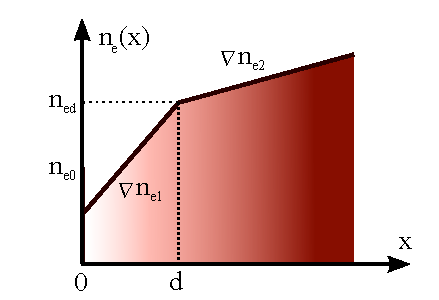
\includegraphics[width=1.0\textwidth]{figures/chap2/ALOHA/figure3}
	\caption{Description of the electronic density profile by two linear profiles
		in front of an antenna. $x=0$ coincides with the position of the
		mouth of the grill.\label{fig:Electron-density-profile} }
\end{marginfigure}

In ALOHA, it is possible to model the plasma density profile by one or two density gradients. The first layer is characterized by a density gradient $\nabla n_{e1}$ and a thickness $d$; the second layer is characterized by a density gradient $\nabla n_{e2}$ of infinite extent, as illustrated in figure \ref{fig:Electron-density-profile}: 
\begin{equation}
\left\{ 
\begin{array}{ll}
n_{e}\left(x\right)=n_{e0}+\nabla n_{e1}\, x & \mbox{for } 0\leq x\leq d\\
n_{e}\left(x\right)=n_{ed}+\nabla n_{e2}\,\left(x-d\right) & \mbox{for }  x>d
\end{array}
\right.
\label{eq:density_profile}
\end{equation}

where $n_{ed}=n_{e0}+\nabla n_{e1}\, d$.


Inside the second layer, the solution of the wave equation (\ref{eq:wave_equation}) for $\tilde{E}_{z}$ is similar to the one found in the case of a single layer since the physical requirement as $x\rightarrow+\infty$ is the same. Inside the first layer, the solution for $\tilde{E}_{z}$ is a combination of Airy and Whittaker functions. The relationship between the both solutions can be found considering that the solutions for the transverse electric and magnetic fields at the interface of both layers $x=d$ have to be continuous and the plasma admittance at the mouth of the antenna can be expressed analytically. Details of the derivation for a 1D case can be found in \citeauthyear{hillairet2010}.


\subsection{Numerical validations}\label{sec:numerical_considerations}

The results of the coupling calculation described in the previous sections depend on the total number of modes $N_{\mbox{modes}}$. In order to determine the minimal number of modes to take into account in order to insure the convergence of ALOHA, the total number of modes has been varied and the results on the C3 antenna compared. This is illustrated in Figure~\ref{fig:RC-E_vs_ne_vs_modes}, where the average reflection coefficient and the average electric field at the grill mouth are plotted versus the electron edge density $n_{e0}$ for the C3 antenna. When three or more modes are used, the results get very
close, indicating that the convergence has been reached. 

%
\begin{figure}[h]
	\begin{centering}
		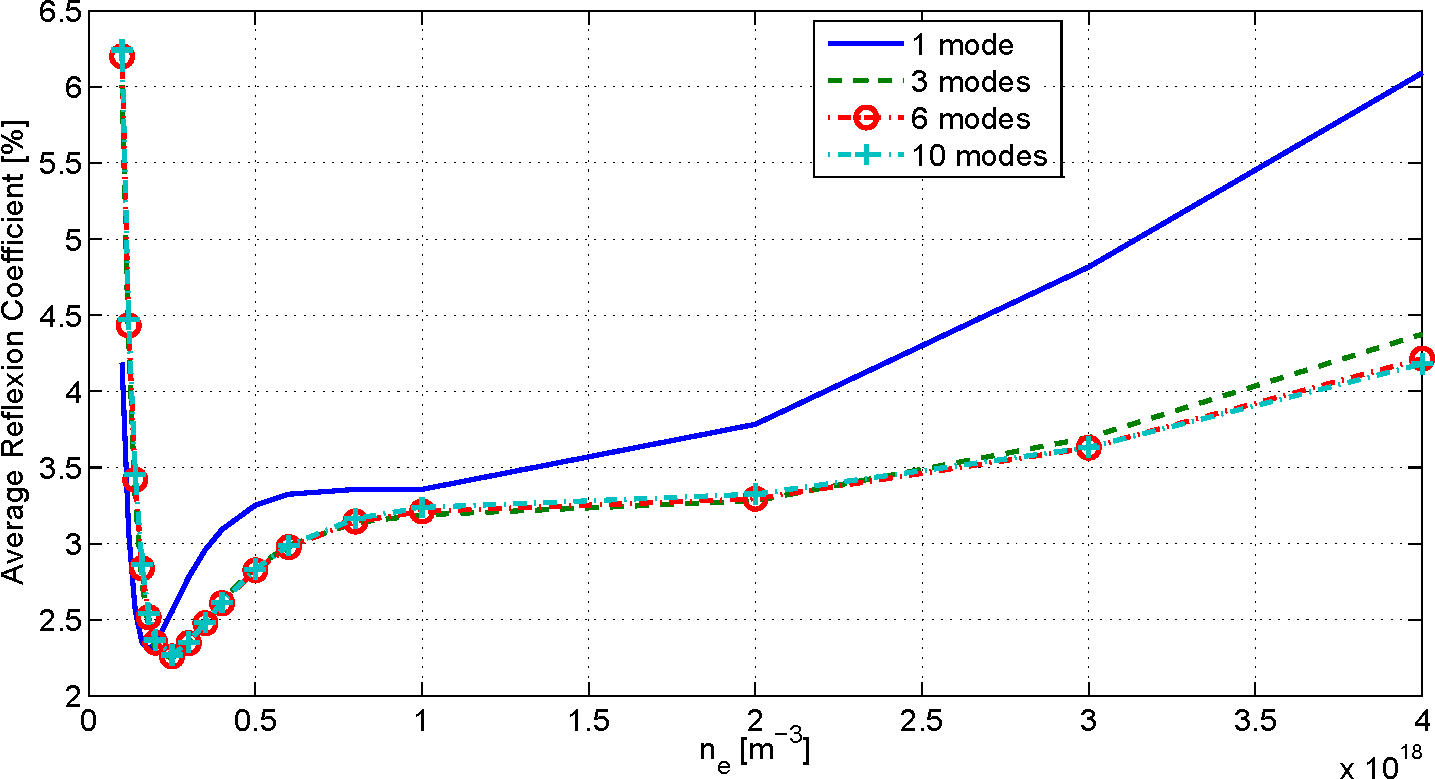
\includegraphics[width=1.0\textwidth]{figures/chap2/ALOHA/figure4a}
		\par\end{centering}
	
	\begin{centering}
		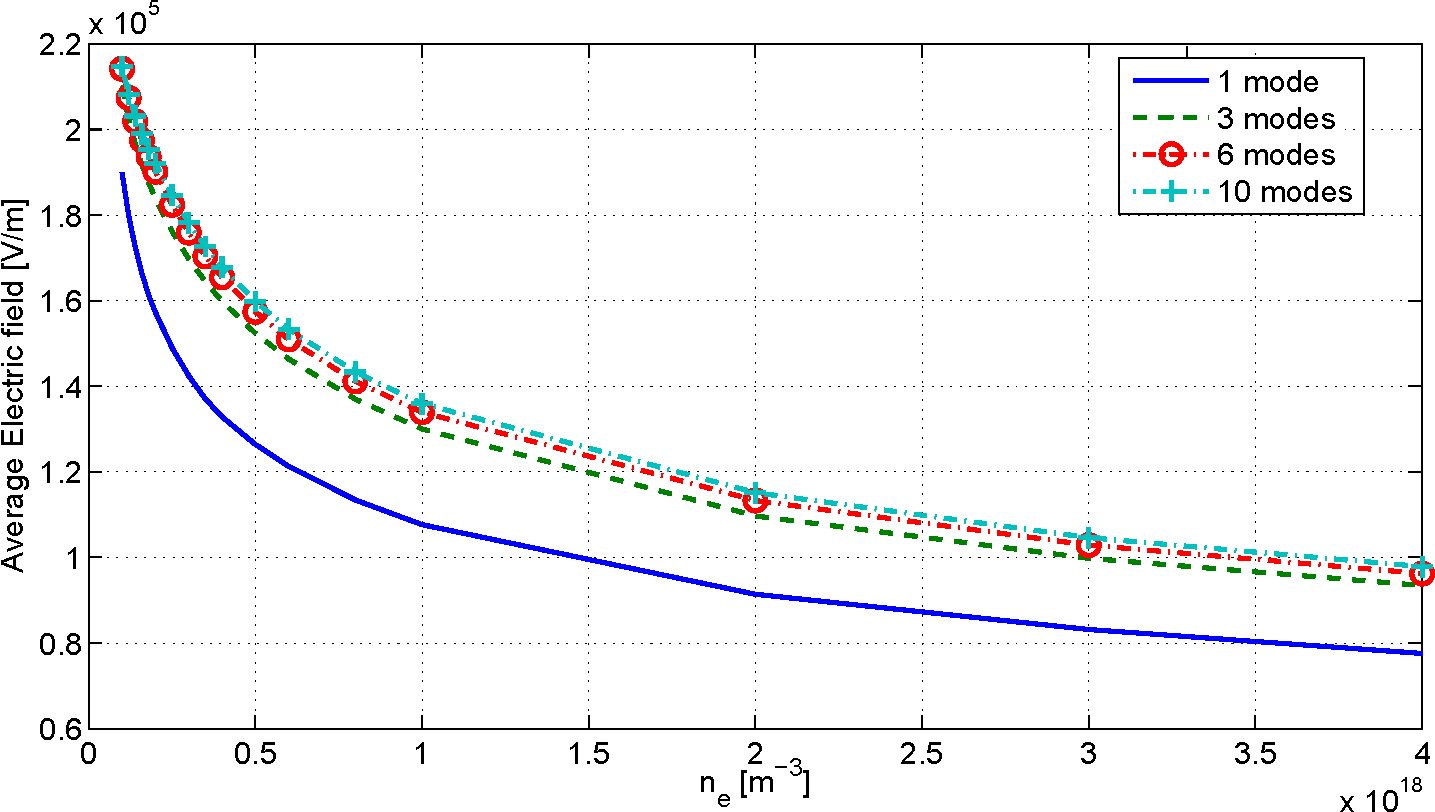
\includegraphics[width=1.0\textwidth]{figures/chap2/ALOHA/figure4b}
		\par\end{centering}
	
	\caption{Reflection coefficient (upper) and average electric
		field at the mouth (lower) vs edge electron density
		for the C3 antenna calculated by ALOHA, for different total number
		of modes taken in account.\label{fig:RC-E_vs_ne_vs_modes} }
	
\end{figure}


In Figure~\ref{fig:Computation-time-versus-modes}, the computation time has been plotted versus the total number of modes $N_{\mbox{modes}}$ for a simple antenna made of 8 independently fed waveguides and for the C3 antenna (57 waveguides per row). As illustrated in the Figure~\ref{fig:Computation-time-versus-modes}, the time complexity of the coupling calculation is function of the number of waveguides and the number of modes taken into account. In both examples, the running time is proportional to the square of the product of the number of waveguides and the number of modes, i.e. $O\left(N_{\mbox{wg}}^{2}\times N_{\mbox{modes}}^{2}\right)$. In the following of this paper, 3 modes were used for all the simulations made with ALOHA. 3 modes are sufficient at low density ( $1.10^{17}\sim20.10^{17}\mbox{\ensuremath{m^{-3}}}$)
which is the density range of interest for this work.

%
\begin{figure}[h]
	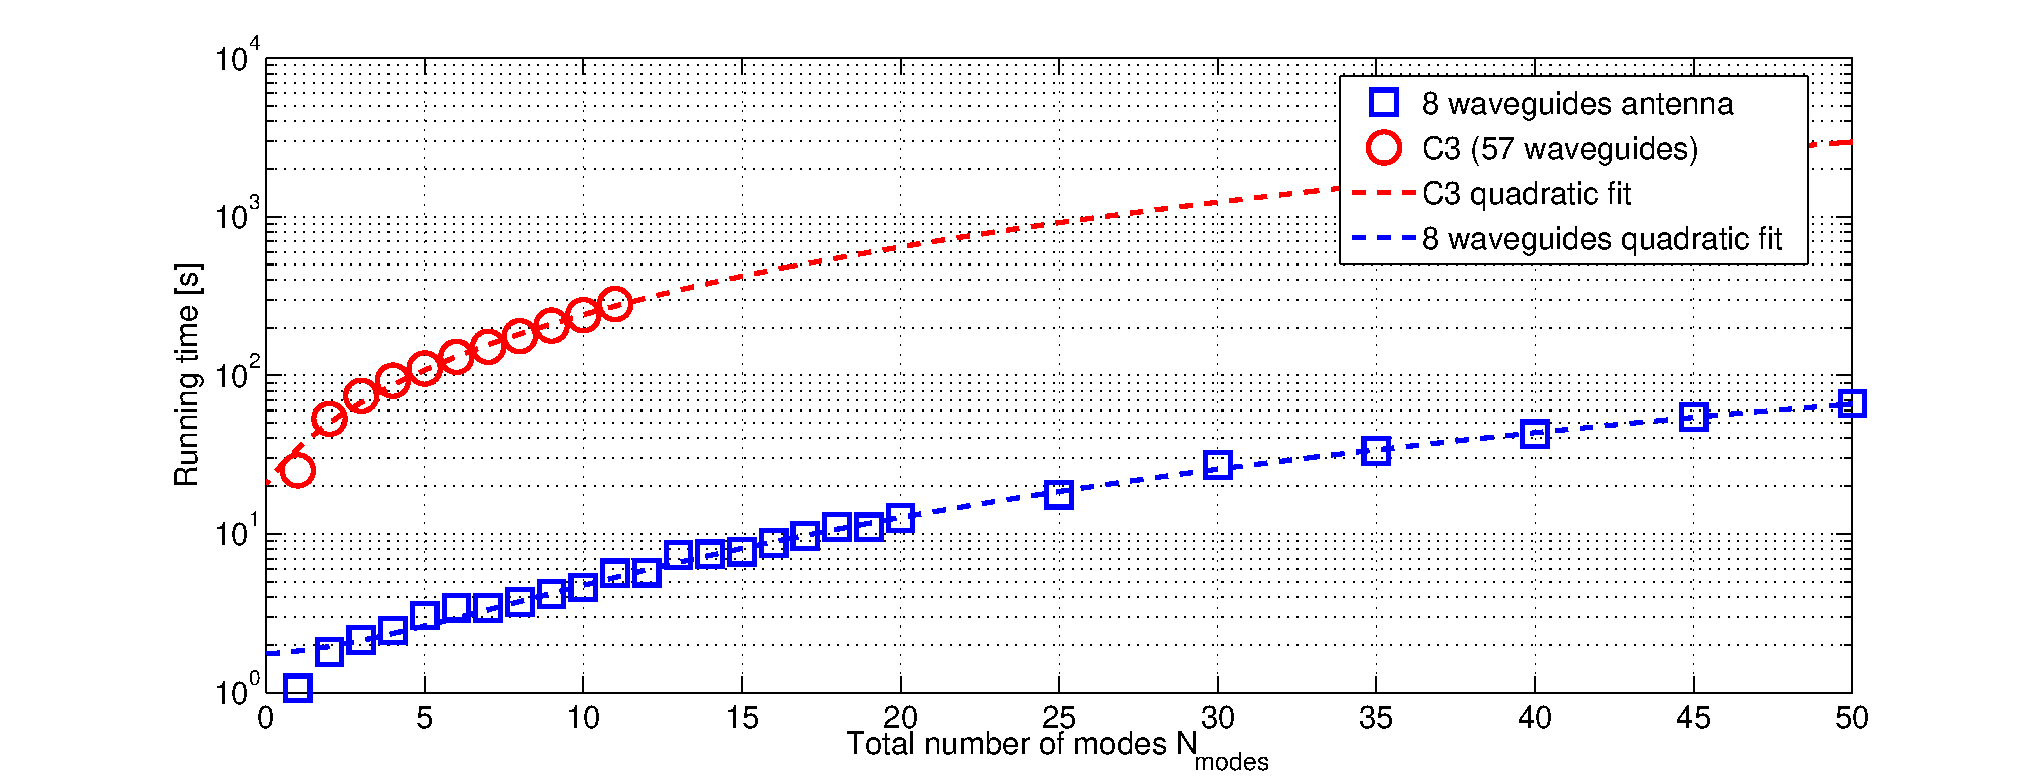
\includegraphics[width=1.0\textwidth]{figures/chap2/ALOHA/figure5}
	\caption{Computation time versus total number of modes for a simple antenna
		made of 8 waveguides and for the C3 antenna. The dashed lines are
		quadratic fit in $N_{\mbox{modes}}^{2}$. \label{fig:Computation-time-versus-modes}}
\end{figure}


When the antenna is large -- that is to say in practical terms when there are more than about thirty waveguides --, the numerical computation of the coupling for a 2D plasma description becomes very difficult. In order to reach the convergence, the precision required on the calculation of the coupling terms in (\ref{eq:coupling_admittance}) leads to a drastic increase of the computational time. To avoid this problem, a solution consists in introducing losses in the vacuum permittivity. This hypothesis changes the diagonal terms of the dielectric tensor ($S'=S-j\delta$ and $P'=P-j\delta$ where $\delta$ is a factor of losses, $\delta\ll1$ and $\delta>0$) and this eliminates the singularities that appear in the expression of the admittance surface given previously. However, the implementation of the analytical solution when losses are introduced is very difficult because of the complex arguments that appear in Whittaker functions. It is then more convenient to numerically solve the differential wave equations by using the finite element method as explained previously. For the sake of illustration, setting $\delta=10^{-2}$ enables to reduce the computational time by more than two order of magnitude without disturbing the antenna response .


\subsection{Summary of this work}
The open-source ALOHA code has been developed to model the Lower Hybrid antenna coupling. In this code, multijunction antennas can be described by any full-wave RF software in order to take into account their detailed geometry. The plasma density layers in front of the antenna can be defined by one or two linear models in order to allow a more realistic description of the scrape-off density profile in front of the antenna. The coupling between the plasma and antenna is treated with either fast and slow waves (ALOHA-2D) or slow wave only (ALOHA-1D) via a surface admittance formulation. The code has also been successfully benchmarked to other codes: TOPLHA \sidecite[+2cm]{milanesio2011}, OLGA \sidecite[+1cm]{preinhaelter2017-1, preinhaelter2018} or FEM codes such as ANSYS HFSS \sidecite{hillairet2019}. The next Section presents some experimental comparisons with experiments performed on Tore Supra.

\clearpage

% #####################################################
% #####################################################
\section{ALOHA Coupling Calculations for Tore Supra LHCD Antennas}\label{sec:ALOHA_TS}
\marginnote{Part of this section are taken from paper \cite{hillairet2009-2}.}
\subsection{Context of this work}
During October and November 2008, dedicated experiments were carried out in Tore Supra in order to compare the measured power reflection coefficients on the C2 and C3 launchers\sidenote{The C2 antenna has been removed from Tore Supra in 2009 and replaced by the Passive-Active Multijunction, labelled C4 (then LH2 in WEST).} with the numerical results from the ALOHA code. In order to avoid possible non-linear effects\cite{petrzilka1987, ekedahl2009}, low power pulses were used, i.e. pulses for which the power density at the mouth of the antenna is less than $2~\si{MW/m}^2$ (corresponding to a total input power of 100~kW). The parameters for pulse $\#43016$ are shown in Fig.~\ref{fig:TS43016}. A large variation of density in front of the antenna between $0.3\times10^{17}~\mathrm{m}^{-3}$ and $13\times10^{17}~\mathrm{m}^{-3}$ was obtained by varying the distance between the last closed flux surface (LCFS) and the antenna during the pulse (cut-off density is $n_{ec}=1.7\times10^{17}~\mathrm{m}^{-3}$). Electron density was measured with the Langmuir probes embedded in to the LH antennas. 

\todo{Refaire la figure}
\begin{figure}[h]
	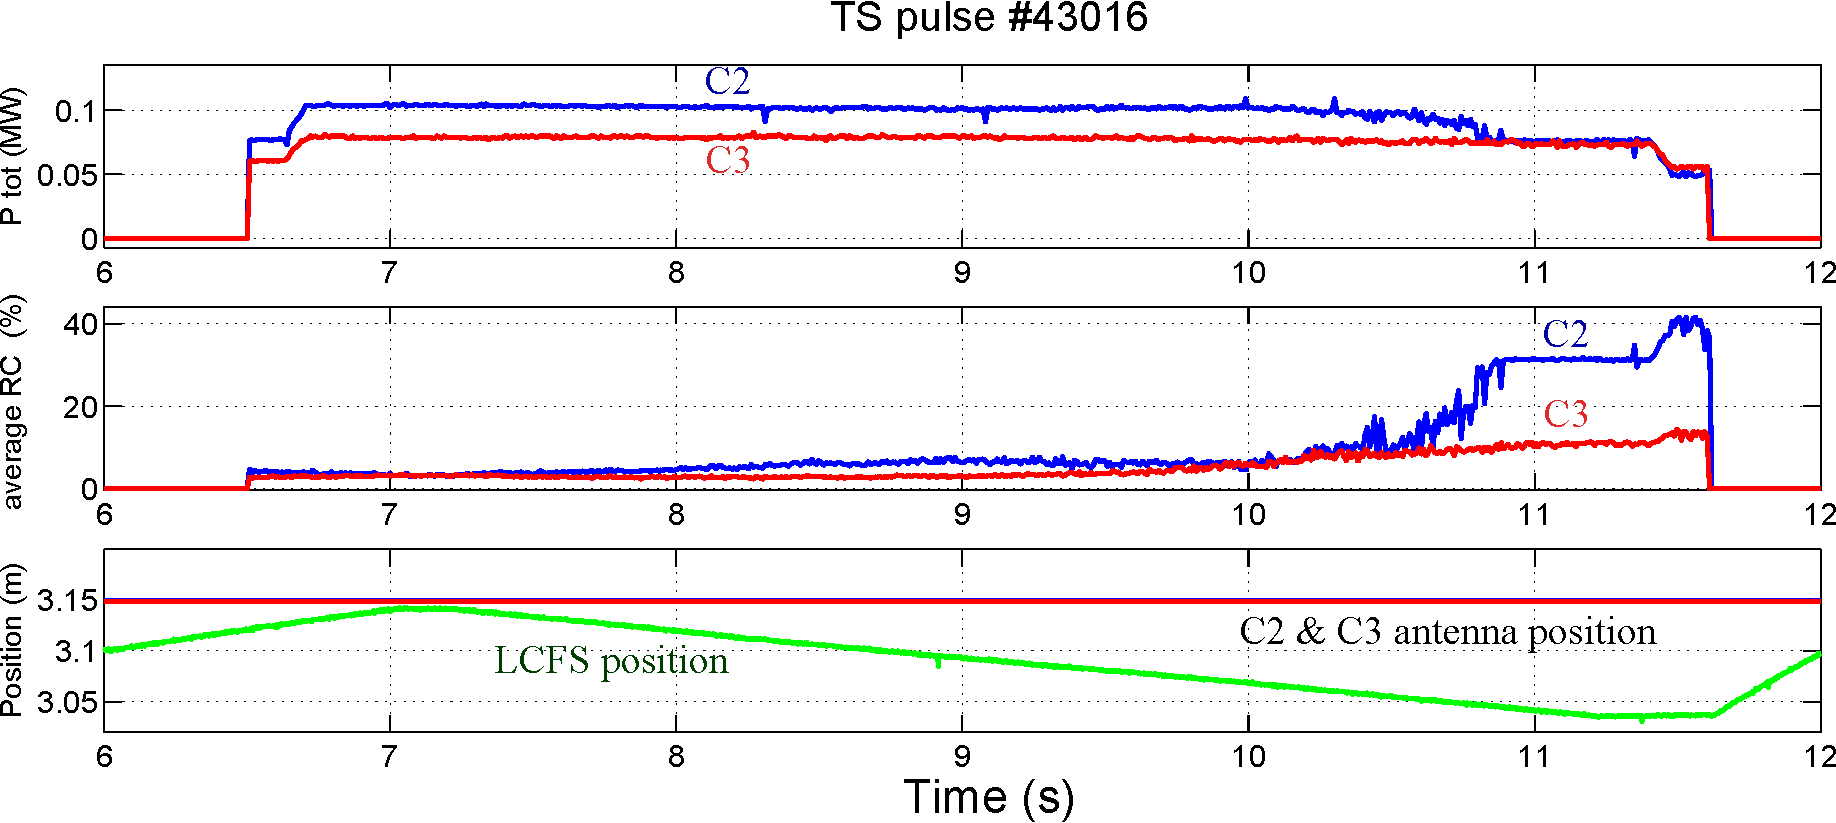
\includegraphics{figures/chap2/Tore_Supra/TS43016}
	\caption{Tore Supra pulse $\#43016$. Top: total power; middle: reflection coefficient; bottom: plasma LCFS and antenna positions.}
	\label{fig:TS43016}
\end{figure}

%Also shown are the poloidal cross sections of the plasma at the time of the RFA measurements at t = 7.05, 9.2 and 10.9 s (strictly speaking these are the poloidal cross sections for 42939 but I found very similar cross sections for all shots). The densities (as well as other RFA parameters like Jsat, Ti and Te) measured for different shots and fixed time are very similar because the plasma density is almost identical for all shots, the difference in the heating power between shots is very small and Ip is constant. The density e-folding increases slightly as the plasma moves from the APL during the shot, which could be explained by the enhancement of the particle transport on the LFS, as demonstrated earlier by the Jamie�s Mach probe measurements.

In ALOHA, the edge plasma is described with a linear electron density profile and no vacuum layer in front of the grill. RFA measurements have been used to estimate typical scrape-off thickness in front of the antennas\cite{kocan2008-1}. The connection lengths $L_{c,LH}$ in front of C2 and C3, corresponding to the distance between protruding side limiters, are known to be $40~\si{cm}$ and $60~\si{cm}$. Assuming that the ratio of the cross-field diffusion coefficient $D_\perp$ and the plasma acoustic velocity $c_s$ is constant in the SOL, and using scrape-off thickness defined as $\lambda_n=\frac{n_{e0}}{\nabla n_{e0}}=\sqrt{\frac{D_\perp L_c}{c_s}}$, one finds that $\lambda_{n,LH}=\sqrt{\frac{L_{c,RFA}}{L_{c,LH}}\lambda_{n,RFA}^2}$. 



% #################################################
% #################################################
% #################################################
\subsection{C2 antenna}
We present here some comparisons between experimental measurements and ALOHA on the Tore Supra C2 antenna. This antenna, installed in 1991, has been removed in 2009 and replaced by a new passive-active multi-junction antenna\cite{guilhem2009,guilhem2011}. The C2 antenna is made of 8 modules. Each module line is a 1-to-4 multi-junction (cf.~Fig~\ref{fig:geometry_TS_LHAntennas}). Permanent built-in phase shifters produce a $90^\circ$ phase difference between each output waveguides on a toroidal line, which produce a nominal peak parallel index of $n_{\parallel,0}=1.82$.

\begin{figure}[h]
	\centering
	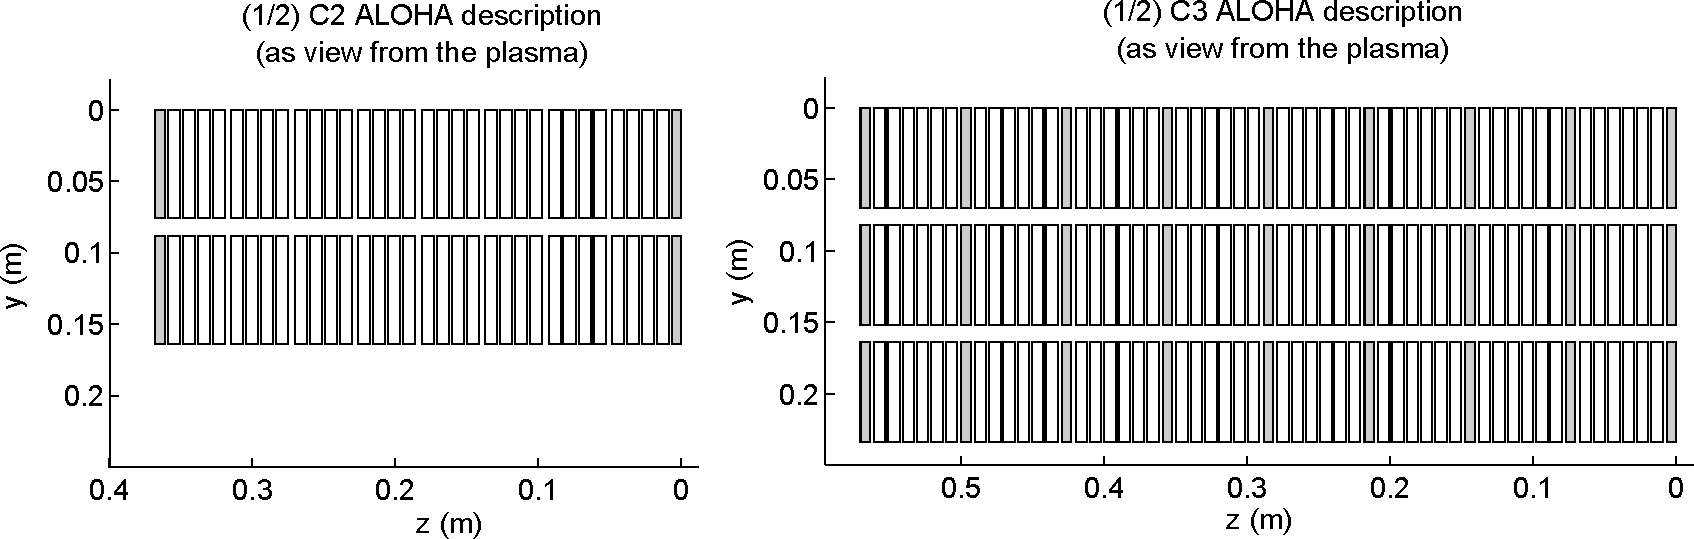
\includegraphics[width=1.0\textwidth]{figures/chap2/Tore_Supra/geometry_TS_LHAntennas}
	\caption{ALOHA description of the upper parts of C2 and C3 antennas . Grey parts symbolizes passive waveguides.}
	\label{fig:geometry_TS_LHAntennas}
\end{figure}

In Figure~\ref{fig:MarkI_mean_RC}, experimental reflection coefficients at different electron densities, measured during Tore Supra pulses \#43014-43016 for 5 upper modules of the C2 antenna are plotted. The density is measured with the nearest Langmuir probe placed at the center of the C2 antenna. Plain black line corresponds to the reflection coefficient calculated with ALOHA for different electron density values $n_{e0}$ at the mouth of the antenna for $\lambda_n=7$~mm. Dotted lines are for$\lambda_n=5$ and $10$~mm. For the C2 antenna, RFA measurements give $\lambda_n$ in $[3.3, 6.5]$~mm, which is in agreement with ALOHA results. 

\begin{figure}[h]
	\centering
	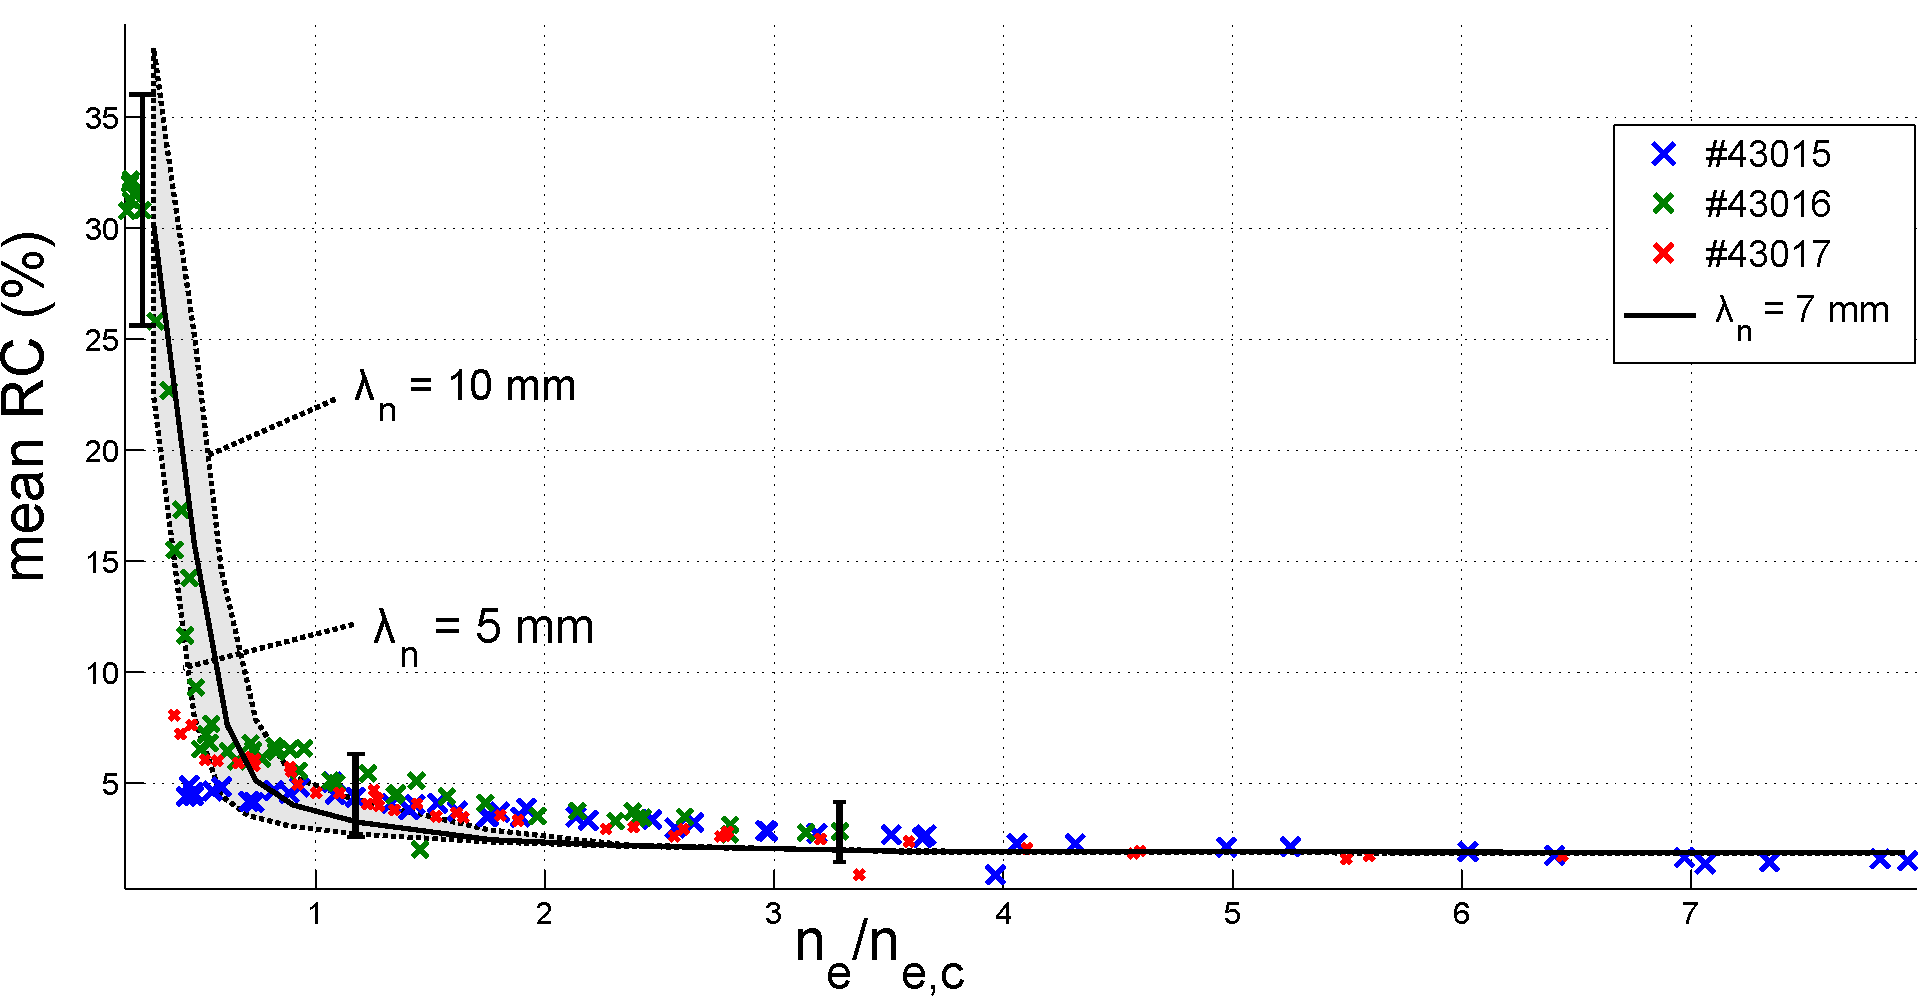
\includegraphics[width=0.95\textwidth]{figures/chap2/Tore_Supra/C2_mean_CR_modBas}
	\caption{Average reflection  coefficient (in percents) versus electron density (normalized to LH cut-off density) for C2 antennas. Measured reflection  coefficient are taken from TS pulses number 43014-43016. Black curve corresponds to a $2~mm$ scrape-off thickness ($\pm 1~mm$).}
	\label{fig:MarkI_mean_RC}
\end{figure}

% #################################################
% #################################################
% #################################################
\subsection{C3 antenna}
C3\sidenote{The antenna has been relabelled LH1 in WEST.} has been installed in 1999 and is also made of 8 modules. Each module is a 1-to-6 multi-junction (cf. Figure~\ref{fig:geometry_TS_LHAntennas}). Permanent built-in phase shifters produce a $90^\circ$ phase difference between each output waveguides on a toroidal line, which produce a nominal peak parallel index of $n_{\parallel,0}=2.02$.

In Figure~\ref{fig:MarkII_mean_RC}, experimental reflection coefficients at different electron densities, measured during Tore Supra pulses \#43014-43016 for the 4 first lower modules of the C3 antenna are plotted. The density is measured with the nearest Langmuir probe placed at the bottom of the C3 antenna. 

\begin{figure}[h]
	\centering
	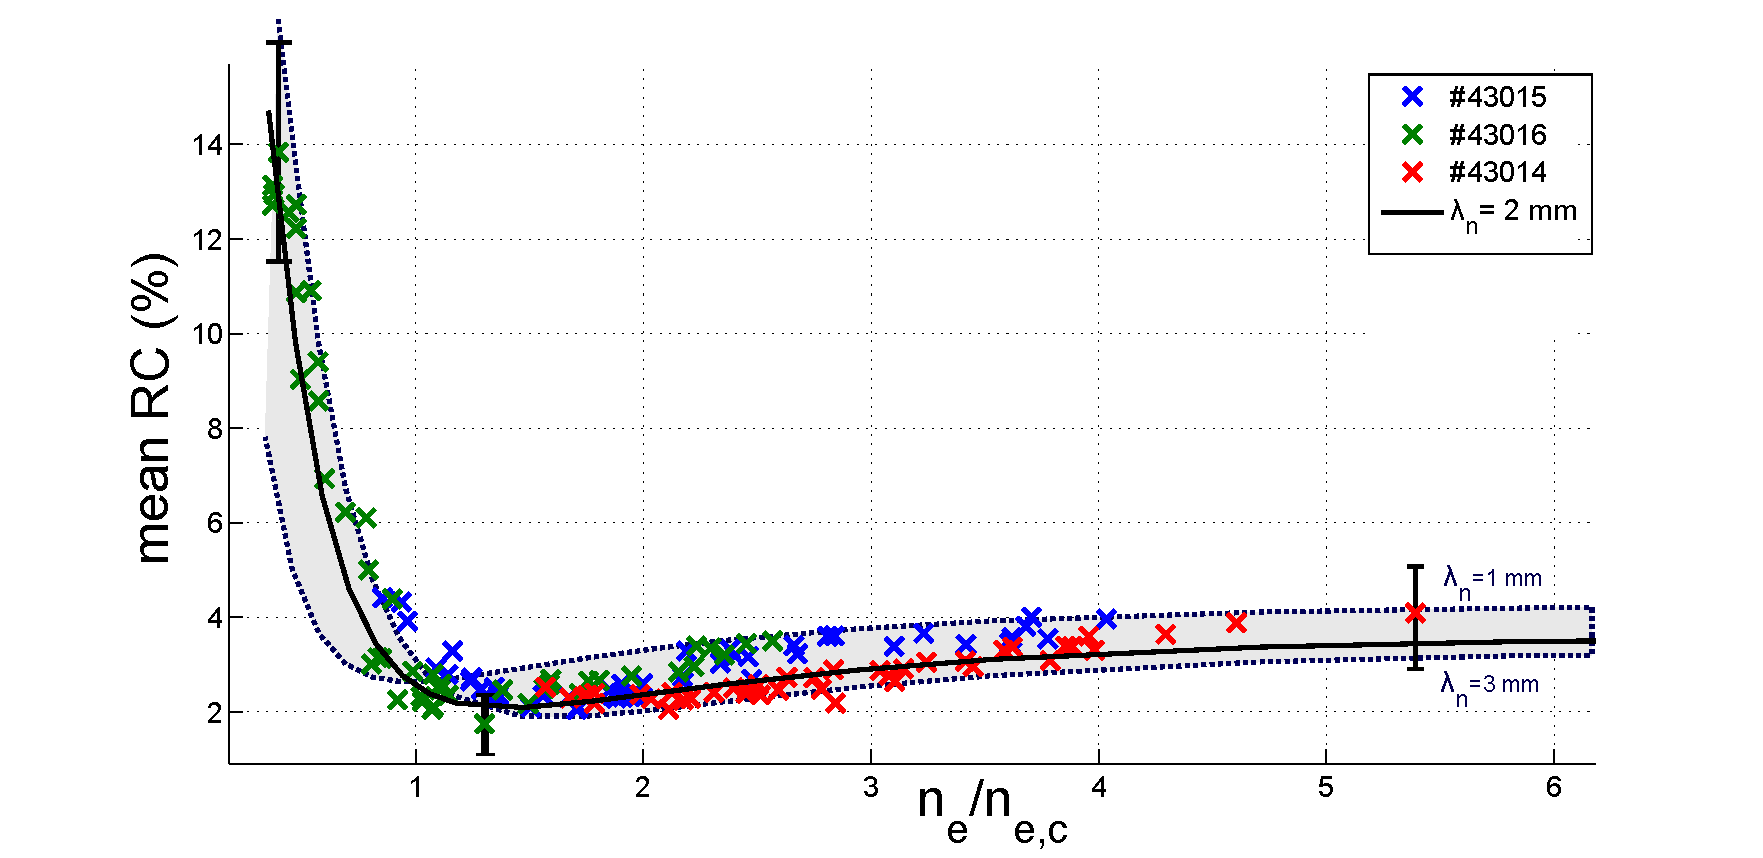
\includegraphics[width=0.95\textwidth]{figures/chap2/Tore_Supra/C3_mean_lowerMod}
	\caption{Average reflection  coefficient (in percents) versus electron density (normalized to LH cut-off density) for C3 antennas. Measured reflection  coefficient are taken from TS pulses number 43014-43016. Black curve corresponds to a $2~mm$ scrape-off thickness ($\pm 1~mm$).}
	\label{fig:MarkII_mean_RC}
\end{figure}




% ##################################################
\subsection{C4 antenna}
\todo{Figures Mélanie}

% ##################################################
\subsection{Summary of this section}

Experimental reflection coefficients at different electron densities, measured during Tore Supra pulses had been compared with the ALOHA code predictions. Results obtained with ALOHA are in good agreement with the experimental measurements for both Tore Supra antennas and shows that ALOHA is an efficient LH predictive tool. 

% ###################################################
% ###################################################
\section{Full-Wave Antenna Coupling}\label{sec:LHCD_FW_antena_coupling}
\marginnote{Part of this section are taken from paper \cite{hillairet2019}.}
\subsection{Context of this work}
During the last two decades, the availability of RF full wave software eased the design of RF antennas, such as ICRF and LHRF antennas. As both software and hardware progressed, modelling has become more and more realistic, reducing the gap between CAD and RF models and accelerating the necessary feedback between mechanical and RF engineers. Nowadays, thermal or mechanical loads can be provided directly from the results of RF simulations inside integrated workflows, which make design phases faster.

As seen in Section~\ref{sec:waves-in-plasma}, when the magnetic field is oriented along the $z$ axis, the plasma facing the antennas can be described in the cold-plasma approximation with the relative permittivity tensor in the $e^{j\omega t}$ time-harmonic convention Eq.(\ref{eq:stix_K}), recalled here:
\begin{equation}
\varepsilon_r 
=
\left(
\begin{array}{ccc}
S & jD & 0 \\
-jD & S & 0 \\
0 & 0 & P
\end{array}
\right)
\label{eq:stix_tensor}
\end{equation}
where the parameters $S$, $D$, $P$ are defined in Eqs.(\ref{eq:stix_SDP}) and depends of the RF frequency, the plasma species and the confining magnetic field. 
%The range of values taken by the $S, D$ and $P$ parameter for typical operational parameters for ICRF and LHRF is illustrated in Fig.\ref{fig:sdp_vs_density}. 
A decade ago, antenna to plasma coupling modelling with commercial full-wave tools was not possible unless some severe simplifications, as they used to not support anisotropic and inhomogeneous dielectric media. Moreover, solving such problems requires large computer resources, which were not easily available since recently. Community codes such as {OLGA} \cite{preinhaelter2017} or {ALOHA} \cite{hillairet2010} (Section~\ref{sec:ALOHA}) and {TOPLHA} \cite{milanesio2012} for LHRF and {ANTITER II} \cite{messiaen2011} or {TOPICA} \cite{lancellotti2006} for {ICRF}, were developed specifically for that purpose. While these tools are generally faster than full-wave modelling since they solve part of the problem in the spectral domain, their Doppelgänger is to assume slab plasma and eventually simplified antenna geometries to keep an analytical formulation of the problem. When dealing with detailed and curved antennas, poloidal and toroidal plasma curvatures or wave scattering by plasma inhomogeneities, 3D numerical approaches become mandatory. 

Regarding coupling performances only, using constant dielectric fast-wave antenna loading has been proved to be a good workaround \cite{messiaen2011-1}. In practice, using high permittivity medium such as (salty) water\cite{messiaen2005} or BaTiO3 solutions\cite{helou2018} are used in laboratory experiments. Hence,  antenna coupling performances have been investigated substituting the plasma load  with a salty water tank in ANSYS HFSS \cite{ravera2012, qin2015} or with BaTiO3 in Microwave CST \cite{bottollier-curtet2011}. Meta-material load had been successfully tested\cite{rustomji2018} for LHRF coupling measurements at low power. 

However, using constant dielectric as radiation medium can't reproduce neither the inhomogeneity produced by increasing density in operational conditions or the medium gyrotropy and anisotropy effects on antenna loading. If these effect are not crucial for coupling calculations, they are for interest for other codes using antenna coupling quantities as input. As an example, if the magnetic field is aligned with the $z$ direction, the radiated spectrum generated by the antenna which depend on the wave number in toroidal $k_z$ and poloidal $k_y$ directions, is an even function of $k_z$ but not of $k_y$ due to gyrotropy\sidecite{messiaen2011, colas2019}.

Since the last decade, full wave codes such as {COMSOL}, Microwave {CST} or {ANSYS} {HFSS} for example, have been able to define propagating medium as anisotropic tensor with eventually negative or complex permittivity, spatial and frequency dependences. This ability allowed coupling calculations of the C-Mod LH launcher\cite{meneghini2009-1}. Recently, the open-source initiative \cite{shiraiwa2017-1} allows modelling RF waves propagation in edge and core plasmas. In all cases, a difficulty arises in the model setup if  geometry is partially taken into account to save resources: in this case, boundary conditions at the edges of the plasma domain need to be defined. Indeed, default radiation or absorbing boundary conditions such as Perfectly Matched Layer (PML) shipped in all these software are not designed to be used directly on the anisotropic material boundaries but instead on isotropic mediums. For antenna to plasma coupling, the plasma medium in which the antenna radiate is at the contrary considered as an semi-infinite medium and should be thus defined with attached ideal absorbing boundary conditions. Specific PML for anisotropic materials such as a magnetized cold plasma have been used in \cite{jacquot2013, colas2019} and mathematically studied in  \cite{becache2017}. Recently in \cite{louche2017}, a 1D cold plasma has been modelled in CST Microwave Studio and compared against analytical solutions. Due to a software limitation to define non-homogeneous medium, a stratified PML has been used to mimic the single pass absorption in a bulk plasma. To obtain a precise solution, a large number of layers are required in the PML. 

Thanks to the collaboration between CEA, ITER and ANSYS, the RF modelling software ANSYS HFSS supports inhomogeneous anisotropic medium since 2016\sidecite{hillairet2019-2}. The purpose of the work presented in this section is not to produce a rigorous approach of the coupling simulation or to model the wave absorption mechanism in the plasma or non-linear effects such as sheaths  on the antenna boundaries. The motivation is to assess the ability of HFSS to describe the usual range of experimental magnetized cold plasma inhomogeneous parameters facing LHRF (sec.\ref{sec:LHRF}) antennas, away from resonances, in order to guide the RF designer during the design phase of an antenna. Due to space constraint, we focuses only on the LHRF case.%, but the treatment of ICRF cases is similar.

\subsection{LHRF Coupling}
As previously seen in Section~\ref{sec:lhcd}, in the Lower Hybrid Current Drive range of frequencies (2-6~GHz) and edge plasma electron densities in current tokamak experiments ($n_e=10^{17}-10^{18}$ $\si{m^{-3}}$), the cold plasma dielectric tensor is mostly diagonal:
 \begin{equation}
 \varepsilon_r 
 \approx
 \left(
 \begin{array}{ccc}
 1 & 0 & 0 \\
 0 & 1 & 0 \\
 0 & 0 & P
 \end{array}
 \right)
 \label{eq:stix_tensor_lhrf}
 \end{equation}
with
\begin{equation}
\varepsilon_{r,zz} = P\approx 1 - \frac{\omega_{pe}^2}{\omega^2} = 1 - \frac{n_e}{n_c}
\end{equation}
where $\omega_{pe}$ and $\omega$ are respectively the plasma and the RF angular frequency and $n_c$ the slow-wave cut-off density defined by:
\begin{equation}
	n_c = \frac{ \varepsilon_0 \omega^2 m_e}{e^2}
	\label{{eq:cutoff_density_lh}}
\end{equation}
In practice, operational plasma parameters lead to  $P\in[-10,0]$. Thus, as  $n_e$ increases, the required mesh length in the full wave simulation should decrease accordingly to match the decrease of the skin depth which depends of both  permittivity (and conductivity). 

In HFSS, using standard PML around such a medium does not give satisfactory results and one should consider instead developing its own PMLs as done in \cite{jacquot2013}. A workaround consists in adding progressively artificial losses, also known as "adiabatic absorbers"\cite{oskooi2008}. If the waves are sufficiently attenuated before they reach the propagation domain boundaries, the edge boundaries can be set as perfect electric conductors. In order not to interfere too much with the coupling results, a non-lossy region is made in front of the antenna (Figure \ref{fig:LH_HFSS}).  A power law of increasing conductivity has been used to attenuate the field, as:
\begin{equation}
\sigma(x) =  
\begin{cases} 
	\alpha_x (x - x_0)^2 & \mbox{if } x \gg 0 \\
	0 & \mbox{otherwise}
\end{cases}	
\end{equation}
with  $\alpha_x$  a scaling parameter and $x_0$ the location of the lossy region limit. Similar  expressions are used  in direction $y$ and $z$  for $\sigma(y)$ and $\sigma(z)$. The function $\sigma(x)$ can be directly set-up in the material editor or as a global parameter, paying attention that the spatial parameters $(x,y,z)$ are the one of the local material coordinates. 

\begin{figure}[h]
	\centering
	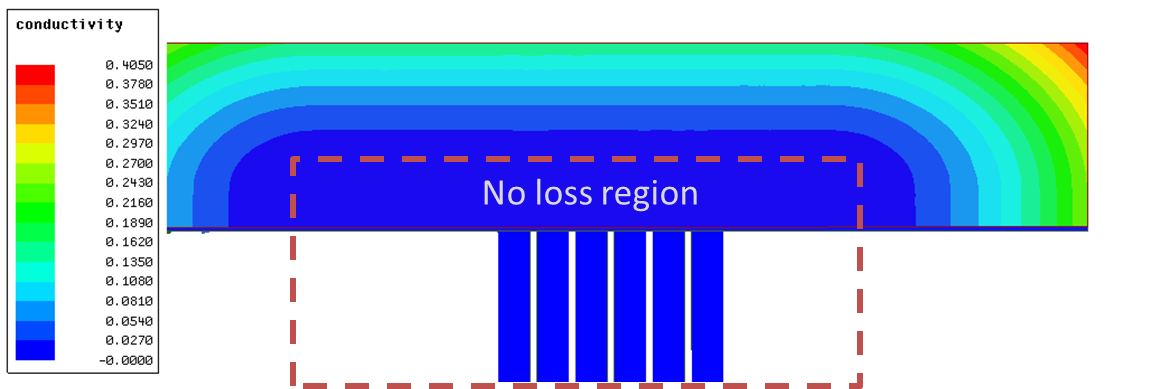
\includegraphics[width=1.0\linewidth]{figures/chap2/LHCD/LH_loss_region}\\
	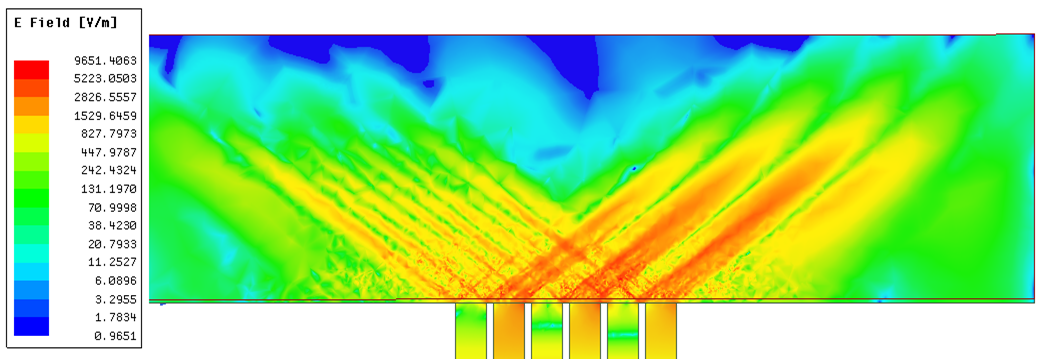
\includegraphics[width=1.0\linewidth]{figures/chap2/LHCD/LH_electric_field_fine_definition}
	\caption{$x-z$ maps in the middle of the waveguide height. Left: conductivity map in the toroidal plane. Right: electric field magnitude (log scale).}
	\label{fig:LH_HFSS}
\end{figure}

As a rule of thumb, a toroidal region at least four times larger than the antenna (toroidal) width and a radial depth at least as large as the antenna (toroidal) width are sufficient, as long as the conductivity law in the radiating region absorb enough power. Without magnetic field tilt angle and without phasing law between waveguide rows, propagation is mainly restricted to the XZ plane and thus the poloidal volume has low influence. A poloidal size of less than twice the height of the antenna is sufficient. In practice, a parametric scan should be first performed on the magnitude of the conductivity law  $\alpha$ until convergence is obtain on the result of interest, for example on the reflection coefficients of the antenna.

\begin{marginfigure}
	\centering
	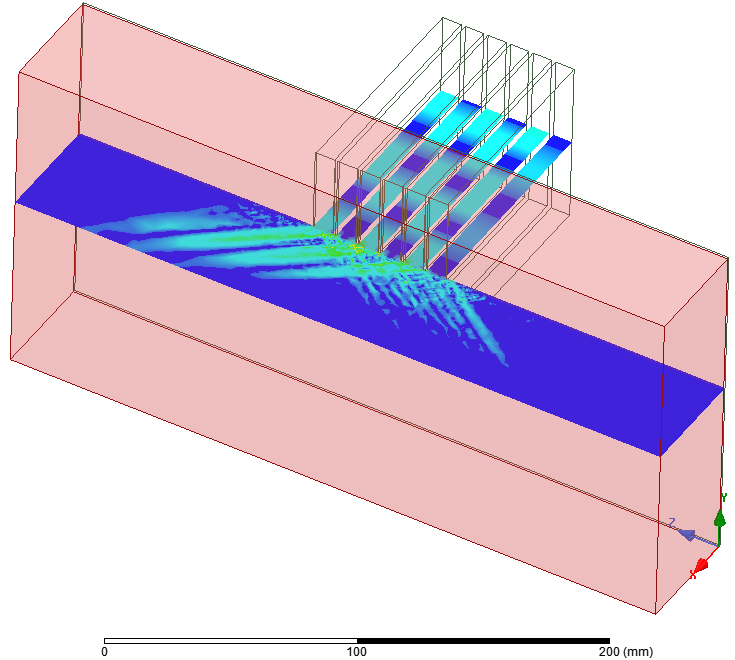
\includegraphics[width=1.0\linewidth]{figures/chap2/LHCD/LH_electric_field}
	\caption{Example of simple LHCD antenna with 6 active waveguides.}
	\label{fig:lhelectricfield}
\end{marginfigure}


In the example illustrated by Figure~\ref{fig:lhelectricfield} and its results presented in Figure~\ref{fig:LH_HFSS}, a 3D LHRF antenna made of six waveguides (76~mm heigh in poloidal direction, 8.5~mm width in toroidal direction and spaced by 2~mm and excited at 3.7~GHz) is facing a small vacuum gap (few millimetres of less) before a linearly increasing density plasma described by:
\begin{equation}
	n_e(x)=n_{e0} \left(1+ \frac{x-d_\mathrm{gap}}{\lambda_n} \right)
\end{equation} 
where $\lambda_n$ is the density scrape-off length and $d_\mathrm{gap}$ the vacuum-gap depth. In order to get physically relevant results, the mesh size should be sufficiently refined to capture  the contribution of high wavenumbers waves propagating in the plasma. In case of LHRF antennas, high toroidal wavenumbers are due to the inevitable spurious lobes generated by LHRF phased array. In the case of the cold plasma in this range of frequencies, the medium wavelength decreases with increasing density. Thus, for a given convergence target criteria (for example in this work the maximum change in the magnitude of the scattering parameters between two consecutive passes is $\Delta S\approx 10^{-3}$ ), the number of elements will increase with the initial edge density. Putting the plasma directly at the contact of the waveguide leads to high order modes (most being evanescent) at the interface between the antenna and the plasma. These modes requires very fine mesh, unless with the reflection inside the antenna would be generally overestimated. A vacuum gap region between the antenna and the plasma speeds-up very much the convergence process since it attenuates these high order modes. This model required around 150~000 elements for a convergence target of $\max|\Delta S|<10^{-3}$, solved in 10-20 minutes on a 64~GB desktop computer. For comparison, similar ALOHA results are obtained in less than a minute. 

The Figure~\ref{fig:LH_fied_spectrum} illustrate the benchmark with the ALOHA code on the electric field and the power density spectrum calculated from the Fourier transform of the electric and magnetic fields at the mouth of the LHRF antenna. The maximum electric field in HFSS is in general lower than in ALOHA because of the smoothing effect of the mesh. The average value is however of the same order. The average Reflection Coefficient (RC) calculated from HFSS matches well ALOHA's calculations when the edge density is higher than the cut-off density (Figure \ref{fig:LH_RC_vs_NeOverNc}). Looking in details, waveguide per waveguide, HFSS results have a reduced RC amplitude  excursion than ALOHA's.  

\begin{figure}[h]
	\centering
	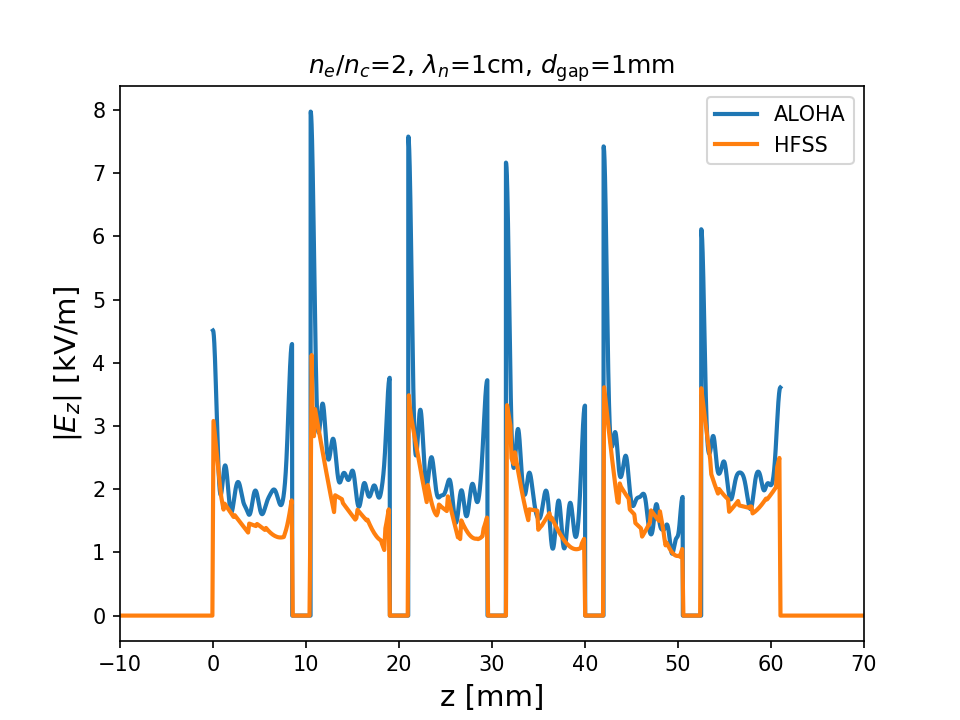
\includegraphics[width=0.8\linewidth]{figures/chap2/LHCD/LH_HFSS_vs_ALOHA_Ez}\\
	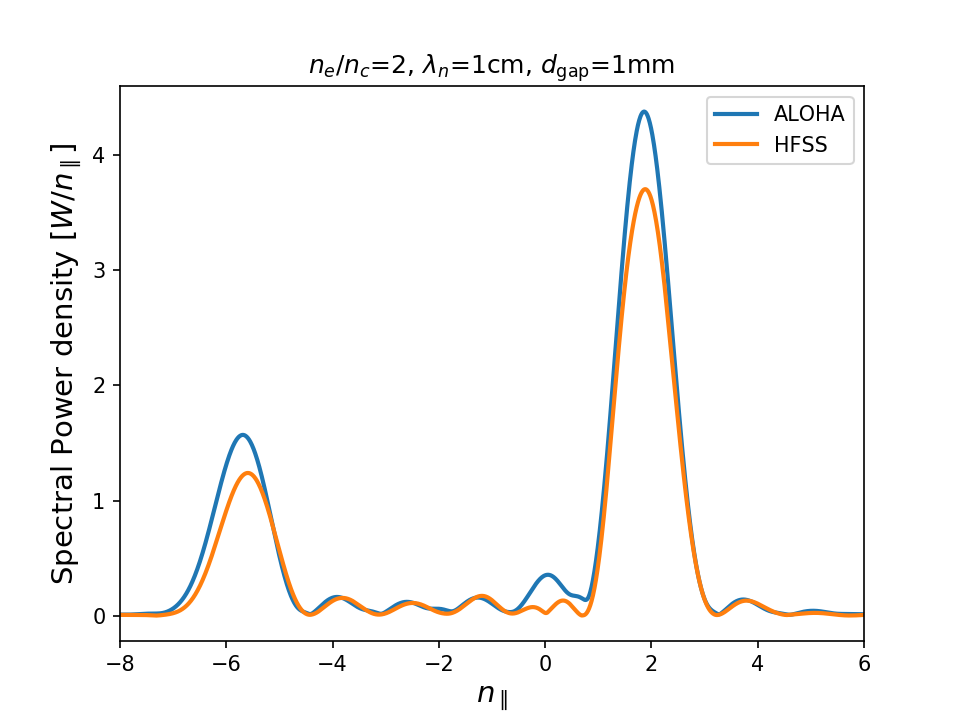
\includegraphics[width=0.8\linewidth]{figures/chap2/LHCD/LH_HFSS_vs_ALOHA_spectrum}
	\caption{Example of comparison between ALOHA and HFSS ($n_e = 2n_c$ , $\lambda_n=1$ cm, 1 mm vacuum gap).  Top: toroidal component of the electric field at the mouth of the antenna. Bottom: Power density spectrum excited by the antenna.}
	\label{fig:LH_fied_spectrum}
\end{figure}

\begin{figure*}[h]
	\centering
	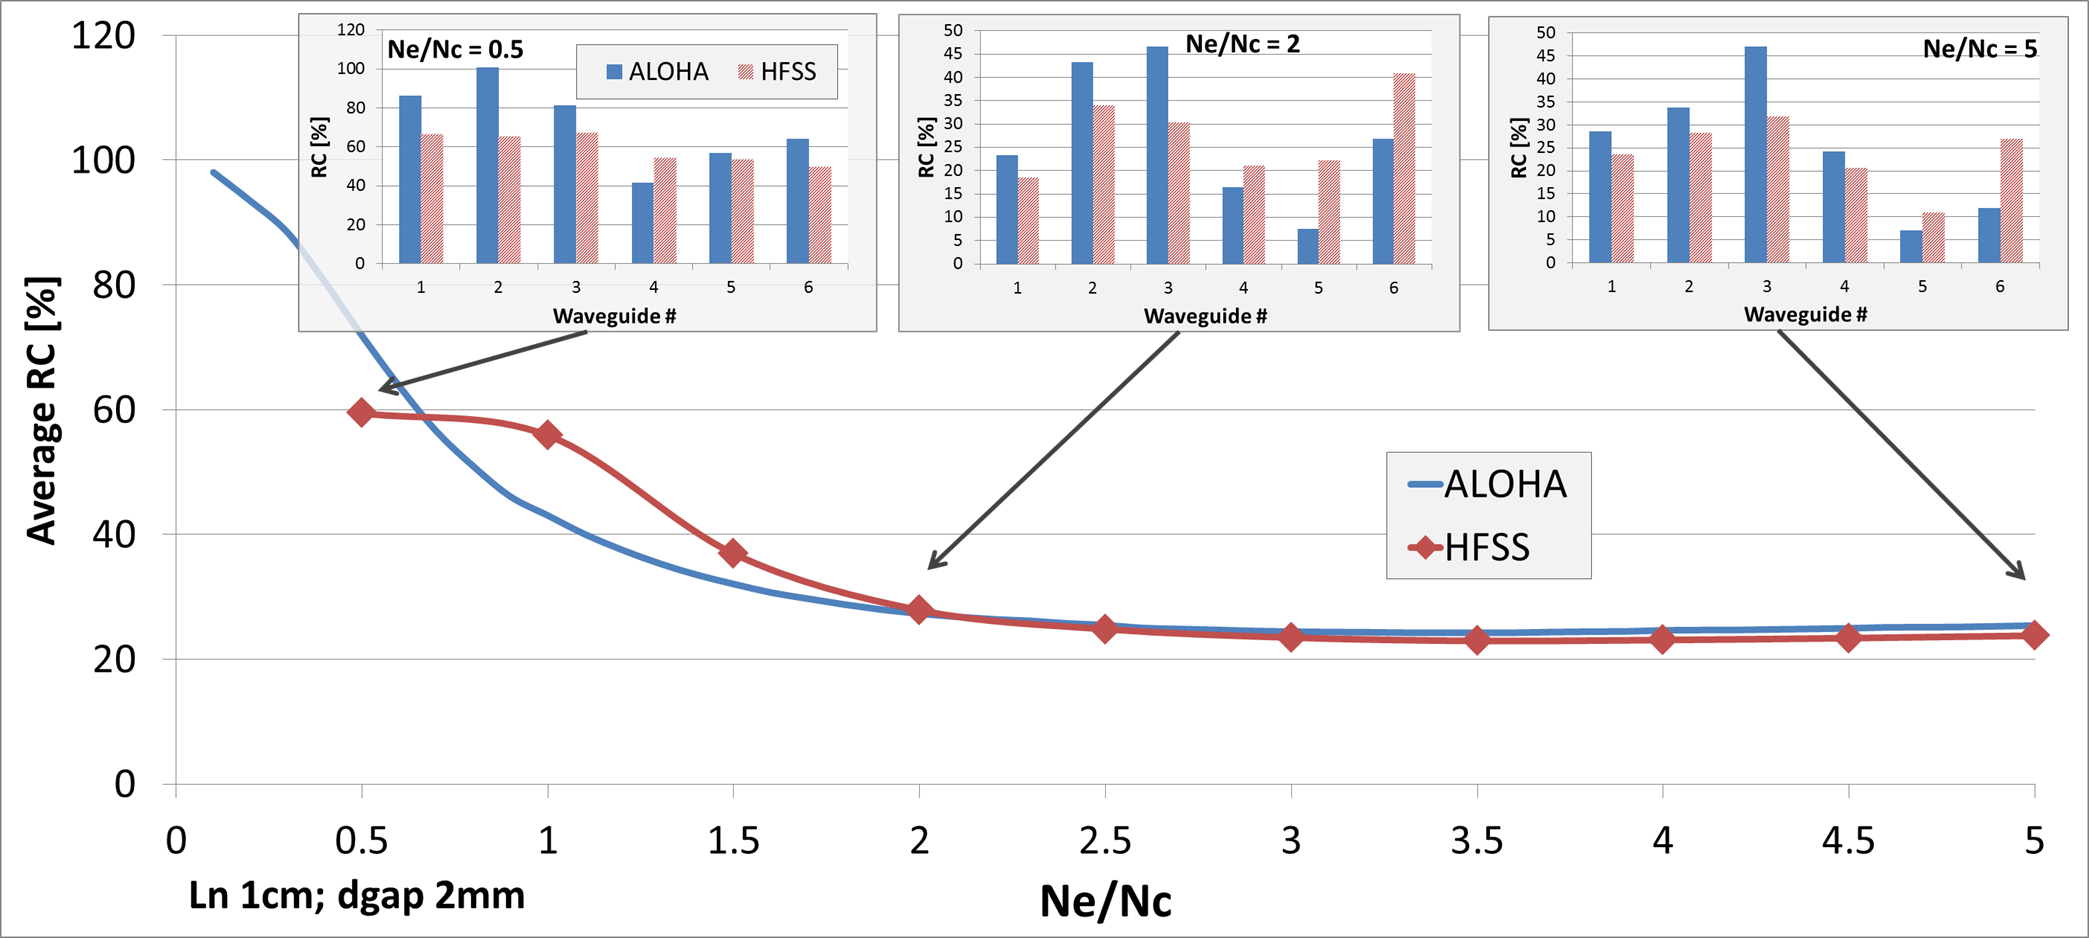
\includegraphics[width=0.98\linewidth]{figures/chap2/LHCD/LH_RC_vs_NeOverNc}
	\caption{Reflection Coefficient (RC) as calculated by ALOHA and HFSS versus the edge density   ($n_e/n_c$) with  $\lambda_n$=1~cm, $d_\mathrm{gap}$=2~mm vacuum gap.}
	\label{fig:LH_RC_vs_NeOverNc}
\end{figure*}

\subsection{ICRF Coupling}
In the Ion Cyclotron range of frequencies (30-60~MHz) for magnetic field in the Tesla range, the relative dielectric permittivity parameter $P$ in Eq.(\ref{eq:stix_tensor}) ranges from $-10^3$ to $-10^5$. Properly mesh the problem requires a node distance of the order of thousandth the wavelength in vacuum. In a domain size of the order of the wavelength, it makes the numerical problem hard to solve on desktop computers. If only the coupling to the fast wave is of interest, the mesh size can be forced to not be smaller than a fraction of the wavelength is the plasma $\lambda_0/\sqrt{\max(|S|, |D|)}$ where $\lambda_0$ if the  wavelength in vacuum. 

However, if anisotropy effects are discarded, using an inhomogeneous equivalent-dielectric isotropic medium  defined as $\varepsilon_{r,eq}=S-D$ \cite{messiaen2011-1}, is a fast and good approximation to determine the antenna coupling performances, in particular S or Z-parameters. Density profile or its equivalent-dielectric permittivity profile, defined from analytical expressions or from tabulated data, can be imported into HFSS  and used into the material properties in order to create an inhomogeneous media. 

%A simplified two-straps antenna has been modelled in ANSYS HFSS and sucessfullt benchmarked to ANTITER~II\cite{messiaen2011}. Detailed assumptions and results will be published in a future paper.

%As an example, a simplified two straps antenna has been modelled in ANSYS  HFSS and in the coupling code ANTITER~II\cite{Messiaen2011}. After a 1~cm vacuum gap between the antenna and the plasma, the electron density increases linearly from $n_{e0}=10^{15} \mathrm{m}^{-3}$ up to a maximum density of $n_{e1}\in [10^{18}, 10^{19}] \mathrm{m}^{-3}$ within a 30~cm distance and stay constant after. Details on the geometry and various assumptions will be published in a dedicated paper.
%In order to get coherent comparisons, the strap thickness was considered as flat as assumed in ANTITER II. Port length has been set long enough to attenuate high-order modes and properly de-embedded. The figure XX illustrates the coupling resistance and various impedances against the maximum density $n_{e1}$ and show a good agreement between HFSS and ANTITER~II.  

\subsection{Summary of this section}
Thanks to the collaboration between CEA, ITER and ANSYS, the RF modelling software ANSYS HFSS supports inhomogeneous anisotropic medium since 2016\sidecite{hillairet2019-2}. The ANSYS HFSS software have been benchmarked for coupling calculations of Lower Hybrid Resonance Frequency to usual edge tokamak cold magnetize plasma conditions. Reflected power and electric field obtained in HFSS agree well with the dedicated LH coupling code ALOHA if absorbing boundary conditions are properly set. In practice, usual edge plasma scenario can be modelled with the requirement of a vacuum gap. The  required memory resources increases with the electron density increase, which can be a practical limitation for high-density scenarios.

For ICRF, the magnitude of the dielectric tensor elements, in particular in the direction parallel to the confinement magnetic field, reach high values which do not allow a direct implementation in HFSS unless using large computing resources. However, if one is only interested in coupling calculation (S/Z-parameters and first order electromagnetic fields), discarding anisotropy effects, using an equivalent dielectric as a loading medium leads to satisfactory results with respect to the IC dedicated coupling code ANTITER II. 

In both case, since it is possible to define inhomogeneous media in HFSS, one can describe equation-based evolution or to directly use numerical data (coming from edge plasma diagnostic such as reflectometers) to model various coupling scenarios. The results obtained can be used by antenna designers to evaluate coupling performances. 

	
	% RF Components
	\chapter{RF Power Devices}
\label{chap:rf_power_devices}
\margintoc

\section{Transmission line}

\section{Matching}

\section{Multipactor}


Magnetic Fusion RF antennas are generally made of copper or silver-coated stainless steels located in vacuum environments. The vacuum sealing with pressurized transmission lines is made with the help of ceramics such as alumina, aluminium nitride, beryllium oxide or diamond. 

All these components are subject to multipactor discharges which increases the electron population (via secondary emission and gas desorption) which in turn may ultimately lead to an avalanche effect and the development of a discharge even at pressures two order of magnitude below Paschen breakdown limit\sidecite{graves2006}. These discharges are generally considered detrimental since they can lead to detuned RF systems, limit the RF power transmission in the plasma and eventually damage RF sources or components. When not detected quickly enough, arcs can lead to surface erosion \sidecite[-0.4cm]{goniche2012-2}, dielectric components metallisation \sidecite{wang2015} or water/air leaks due to punctured components such as bellows \sidecite{mayoral2007} or vacuum windows \sidecite{neuber1998, neuber2007, hillairet2015}. 

In some cases however, multipactor-induced discharges can be desired for vacuum RF conditioning during short RF pulses and at moderate power\sidecite{goniche2012-2, wang2015, halbritter1982, ekedahl1998}. Moreover, these RF systems are subjected to the high magnetic field environment of the experiments in the Tesla range. The presence of magnetic field affects the electron trajectories and thus the multipactor resonances. On tokamaks, the electron motion is strongly constrained around the magnetic field lines which reduce the effects of loss mechanisms such as diffusion and increases electron impact ionization and thus the build-up of glow discharges. Finally, at the difference of RF payloads in satellite, the antenna surfaces can be polluted during operation with particles resulting from the strong interaction of the energetic particles with the walls of the tokamak, which may alter the surface characteristics such as secondary emission. This paper reviews the work performed in the fusion research community on multipactor discharges for two kinds of RF systems with their practical implications on power delivery into the plasma. The Ion Cyclotron Resonance Heating (ICRH), which uses coaxial lines in the MHz range of frequency, is presented in the next section. The Lower Hybrid Current Drive (LHCD) systems, which uses rectangular waveguides in the GHz range of frequency is discussed in section 3. 




\section{RF Contacts}

\section{RF Devices}
\subsection{Mode Converter}
\subsubsection{ITER Mode Converter}

\subsection{Multijunction}

\subsubsection{Tore Supra/WEST LHCD Antennas}

\subsubsection{ITER LHCD Antenna}

\subsection{RF Windows}
\subsubsection{ITER RF Windows}


	
	% Education
	\chapter{Fusion Education}

\section{Master Fusion}
\section{Com grand public}
\section{ITER Robots}
\section{Dim tokamak?}
	
	%----------------------------APPENDIX------------------------------------------------------------
	\appendix % From here onwards, chapters are numbered with letters, as is the appendix convention
	
	\pagelayout{wide} % No margins
	\addpart{Appendix}
	\pagelayout{margin} % Restore margins
	
	%	\setchapterstyle{lines}
\labpage{appendix}

\chapter{Appendix 1}
\section{Section 1}

	%	
	%	

	
	%----------------------------------------------------------------------------------------
	
	\backmatter % Denotes the end of the main document content
	
	\setchapterstyle{plain} % Output plain chapters from this point onwards
	
	%----------------------------------------------------------------------------------------
	%	BIBLIOGRAPHY
	%----------------------------------------------------------------------------------------
	%%%% Main bibliography of the document
	% The bibliography needs to be compiled with biber 	
	\defbibnote{bibnote}{Here are the references in alphabetical order.\par\bigskip} % Prepend this text to the bibliography
	% Use the "nyt" sorting for the bibliography
	\begin{refcontext}[sorting=nyt]
		\printbibliography[heading=bibintoc, title=Bibliography, prenote=bibnote] 
	\end{refcontext}

	\newpage
	\chapter{Publications}
	%%%%% Bibliography of my 1st author publications
	\begin{refsection}[first_author_papers.bib]
		\section*{First Author References}
		\nocite{*}
		\printbibliography[heading=none]
	\end{refsection}

	\section*{Conference and Journal Editorial Work}
	\begin{itemize}
		\item Editor of the \href{https://www.epj-conferences.org/articles/epjconf/abs/2017/26/contents/contents.html}{22th Topical Conference on Radio-Frequency Power in Plasmas}, Aix-en-Provence, France, May 30 - June 2, 2017.
		\item Guest Editor with Alf Köhn (University of Stuttgart) of \href{https://iopscience.iop.org/journal/0031-9120/page/Spotlight-on-Nuclear-Fusion}{IOP "Spotlight on Nuclear Fusion"}.
	\end{itemize}
	
	\section*{Patent}

	\begin{itemize}
		\item Chen, Z., Hillairet, J., 2017. Dispositif De Manoeuvre D’un Actionneur Dispose Dans Une Enceinte Fermee Au Travers D’une Paroi De L’enceinte. \href{https://bases-brevets.inpi.fr/fr/document/FR3066944.html?s=1587045453863&p=5&cHash=9dd74066794d8b15bf32b0ef194d0d86}{FR3066944}~\cite{chen2017-4}.
	\end{itemize}
		
	
	\newpage
	\chapter{Encadrement}
	\section*{Thèses encadrées}
	\begin{itemize}
	\item Nicolas Fil, \textit{Characterization and modelling of the secondary electron emission properties under magnetic field for high power RF systems subject to Multipactor effect}. Institut Supérieur de l'Aéronautique et de l'Espace - Université Toulouse, 2017. 
	
	\item Zhaoxi Chen. \textit{Mechanical and Materials Development of Radio-Frequency Contact for the ITER Ion Cyclotron Resonance Heating Antenna}. Université Toulouse III - Paul Sabatier, 2018.
	
	\item Walid Helou. \textit{Design and operation of antennas at the ion cyclotron and lower hybrid range of frequencies for nuclear fusion reactors}. Aix-Marseille University, 2018.

		\item Adrien Plaçais, \textit{Modélisation et mesures de l'émission secondaire de diélectriques et des phénomènes multipactor en présence de champ magnétique pour la fusion nucléaire contrôlée et le spatial}. Institut Supérieur de l'Aéronautique et de l'Espace - Université Toulouse, 2020 (prévue).
	
	\end{itemize}

	\section*{Stages de Master 2 encadrés}
	\begin{itemize}
		\item Mélanie Preynas, \textit{Développement d’un nouveau module pour le code de couplage ALOHA}, 2009.
		\item Michal Kazda, \textit{Study of the coupling properties of a Passive-Active Multijunction Lower Hybrid antenna with tokamak plasma}, 2010.
		\item François Farthouat, \textit{Conception d'un dispositif de réglage du système optique associé à un gyrotron}, 2010 (co-encadré avec Elodie Corbel).
		\item Pierre-Etienne Marx, \textit{Calcul d'admittance de surface pour l'onde lente à la fréquence hybride basse dans un plasma}, 2011.
		\item Walid Helou, \textit{Etude d’un nouveau concept d’antennes forte puissance à la fréquence hybride basse (LH) pour des réacteurs à fusion nucléaire}, 2012.
%		\item Laurent Valade, \textit{Modelling of heat loads on RF antennas, due to parasitic absorption of Lower Hybrid power in tokamak plasmas}, 2012 (co-encadré avec Annika Ekedahl).
		\item Nicolas Fils, \textit{Modélisation des propriétés d'émission secondaire de composants RF haute puissance}, 2014
		\item Adrien Plaçais, \textit{Modélisation de l'émission secondaire de diélectriques et des phénomènes multipactor en présence de champ magnétique}, 2017.
	\end{itemize}


	%%%%% Copy of 1st author publications
	\if\addpublications1
	\chapter{First Author Publications}
	
	\section{LHCD}
	
		\includepdf[nup=2x2, pages=-, fitpaper=true, linktodoc=true]
		{publications/LHCD/Hillairet et al._2009_Modeling of lower hybrid antennas using the {ALOHA} code and comparisons with Tore Supra experiments.pdf}
		
		\includepdf[nup=2x2, pages=-, fitpaper=true, linktodoc=true]
		{publications/LHCD/Hillairet et al._2010_ALOHA an Advanced LOwer Hybrid Antenna coupling code.pdf}
		
		\includepdf[nup=2x2, pages=-, fitpaper=true, linktodoc=true]
		{publications/LHCD/Hillairet et al._2011_RF modeling of the ITER-relevant lower hybrid antenna.pdf}
		
		\includepdf[nup=2x2, pages=-, fitpaper=true, linktodoc=true]
		{publications/LHCD/Hillairet et al._2012_Design and testing of a 5GHz TE10 TE30 mode conver.pdf}
		
		\includepdf[nup=2x2, pages=-, fitpaper=true, linktodoc=true]
		{publications/LHCD/Hillairet et al._2012_Lower Hybrid antennas for nuclear fusion experiments.pdf}
		
		\includepdf[nup=2x2, pages=-, fitpaper=true, linktodoc=true]
		{publications/LHCD/Hillairet et al._2013_Recent progress on lower hybrid current drive and implications for ITER.pdf}
		
		\includepdf[nup=2x2, pages=-, fitpaper=true, linktodoc=true]
		{publications/LHCD/Hillairet et al._2015_Design and tests of 500kW RF windows for the ITER LHCD system.pdf}
		
		\includepdf[nup=2x2, pages=-, fitpaper=true, linktodoc=true]
		{publications/LHCD/Hillairet et al._2019_Lower hybrid range cold magnetized plasma coupling in ANSYS HFSS.pdf}
		
	\section{ICRH}
	
		\includepdf[nup=2x2, pages=-, fitpaper=true, linktodoc=true]
		{publications/ICRH/Hillairet et al._2015_Ion cyclotron resonance heating systems upgrade toward high power and CW.pdf}
		
		\includepdf[nup=2x2, pages=-, fitpaper=true, linktodoc=true]	
		{publications/ICRH/Hillairet et al._2015_R&D activities on RF contacts for the ITER ion cyclotron resonance heating launcher.pdf}
		
		\includepdf[nup=2x2, pages=-, fitpaper=true, linktodoc=true]
		{publications/ICRH/Hillairet et al._2018_Radiofrequency and mechanical tests of silver coated CuCrZr contacts for the ITER ion cyclotron antenna.pdf}
		
		\includepdf[nup=2x2, pages=-, fitpaper=true, linktodoc=true]
		{publications/ICRH/Hillairet_2019_RF Network Analysis of the WEST ICRH Antenna with the Open-Source Python.pdf}
	
	\section{Multipactor}
	
		\includepdf[nup=2x2, pages=-, fitpaper=true, linktodoc=true]
		{publications/Multipactor/Hillairet et al._2017_Multipactor in High Power Radio-Frequency Systems for Nuclear Fusion.pdf}
	
	\section{Teaching and Outreaching}
	
		\includepdf[nup=2x2, pages=-, fitpaper=true, linktodoc=true]	
		{publications/TeachingOutreaching/Hillairet et al._2019_Protecting Fusion Reactors from Extreme Heat.pdf}
		
		\includepdf[nup=2x2, pages=-, fitpaper=true, linktodoc=true]
		{publications/TeachingOutreaching/Hillairet et al._2020_Radio-frequency hands-on for nuclear fusion Master's sudents.pdf}
		
		\includepdf[nup=2x2, pages=-, fitpaper=true, linktodoc=true]	
		{publications/TeachingOutreaching/Martins et al._2020_ITER robots.pdf}
	
	\fi
	

	


%	%----------------------------------------------------------------------------------------
%	%	NOMENCLATURE
%	%----------------------------------------------------------------------------------------
%	
%	% The nomenclature needs to be compiled on the command line with 'makeindex main.nlo -s nomencl.ist -o main.nls' from the template directory
%	
%	\nomenclature{$c$}{Speed of light in a vacuum inertial frame}
%	\nomenclature{$h$}{Planck constant}
%	
%	\renewcommand{\nomname}{Notation} % Rename the default 'Nomenclature'
%	\renewcommand{\nompreamble}{The next list describes several symbols that will be later used within the body of the document.} % Prepend this text to the nomenclature
%	
%	\printnomenclature % Output the nomenclature
%	
%	%----------------------------------------------------------------------------------------
%	%	GLOSSARY
%	%----------------------------------------------------------------------------------------
%	
%	% The glossary needs to be compiled on the command line with 'makeglossaries main' from the template directory
%	
%	\newglossaryentry{computer}{
%		name=computer,
%		description={is a programmable machine that receives input, stores and manipulates data, and provides output in a useful format}
%	}
%	
%	% Glossary entries (used in text with e.g. \acrfull{fpsLabel} or \acrshort{fpsLabel})
%	\newacronym[longplural={Frames per Second}]{fpsLabel}{FPS}{Frame per Second}
%	\newacronym[longplural={Tables of Contents}]{tocLabel}{TOC}{Table of Contents}
%	
%	\setglossarystyle{listgroup} % Set the style of the glossary (see https://en.wikibooks.org/wiki/LaTeX/Glossary for a reference)
%	\printglossary[title=Special Terms, toctitle=List of Terms] % Output the glossary, 'title' is the chapter heading for the glossary, toctitle is the table of contents heading
	
%	%----------------------------------------------------------------------------------------
%	%	INDEX
%	%----------------------------------------------------------------------------------------
%	
%	% The index needs to be compiled on the command line with 'makeindex main' from the template directory
%	
%	\printindex % Output the index
	
	%----------------------------------------------------------------------------------------
	%	BACK COVER
	%----------------------------------------------------------------------------------------
	
	% If you have a PDF/image file that you want to use as a back cover, uncomment the following lines
	
	%\clearpage
	%\thispagestyle{empty}
	%\null%
	%\clearpage
	%\includepdf{cover-back.pdf}
	
	%----------------------------------------------------------------------------------------


\end{document}
